% Options for packages loaded elsewhere
\PassOptionsToPackage{unicode}{hyperref}
\PassOptionsToPackage{hyphens}{url}
\PassOptionsToPackage{dvipsnames,svgnames,x11names}{xcolor}
%
\documentclass[
  letterpaper,
  DIV=11,
  numbers=noendperiod]{scrreprt}

\usepackage{amsmath,amssymb}
\usepackage{iftex}
\ifPDFTeX
  \usepackage[T1]{fontenc}
  \usepackage[utf8]{inputenc}
  \usepackage{textcomp} % provide euro and other symbols
\else % if luatex or xetex
  \usepackage{unicode-math}
  \defaultfontfeatures{Scale=MatchLowercase}
  \defaultfontfeatures[\rmfamily]{Ligatures=TeX,Scale=1}
\fi
\usepackage{lmodern}
\ifPDFTeX\else  
    % xetex/luatex font selection
\fi
% Use upquote if available, for straight quotes in verbatim environments
\IfFileExists{upquote.sty}{\usepackage{upquote}}{}
\IfFileExists{microtype.sty}{% use microtype if available
  \usepackage[]{microtype}
  \UseMicrotypeSet[protrusion]{basicmath} % disable protrusion for tt fonts
}{}
\makeatletter
\@ifundefined{KOMAClassName}{% if non-KOMA class
  \IfFileExists{parskip.sty}{%
    \usepackage{parskip}
  }{% else
    \setlength{\parindent}{0pt}
    \setlength{\parskip}{6pt plus 2pt minus 1pt}}
}{% if KOMA class
  \KOMAoptions{parskip=half}}
\makeatother
\usepackage{xcolor}
\ifLuaTeX
  \usepackage{luacolor}
  \usepackage[soul]{lua-ul}
\else
  \usepackage{soul}
  
\fi
\setlength{\emergencystretch}{3em} % prevent overfull lines
\setcounter{secnumdepth}{5}
% Make \paragraph and \subparagraph free-standing
\makeatletter
\ifx\paragraph\undefined\else
  \let\oldparagraph\paragraph
  \renewcommand{\paragraph}{
    \@ifstar
      \xxxParagraphStar
      \xxxParagraphNoStar
  }
  \newcommand{\xxxParagraphStar}[1]{\oldparagraph*{#1}\mbox{}}
  \newcommand{\xxxParagraphNoStar}[1]{\oldparagraph{#1}\mbox{}}
\fi
\ifx\subparagraph\undefined\else
  \let\oldsubparagraph\subparagraph
  \renewcommand{\subparagraph}{
    \@ifstar
      \xxxSubParagraphStar
      \xxxSubParagraphNoStar
  }
  \newcommand{\xxxSubParagraphStar}[1]{\oldsubparagraph*{#1}\mbox{}}
  \newcommand{\xxxSubParagraphNoStar}[1]{\oldsubparagraph{#1}\mbox{}}
\fi
\makeatother

\usepackage{color}
\usepackage{fancyvrb}
\newcommand{\VerbBar}{|}
\newcommand{\VERB}{\Verb[commandchars=\\\{\}]}
\DefineVerbatimEnvironment{Highlighting}{Verbatim}{commandchars=\\\{\}}
% Add ',fontsize=\small' for more characters per line
\usepackage{framed}
\definecolor{shadecolor}{RGB}{241,243,245}
\newenvironment{Shaded}{\begin{snugshade}}{\end{snugshade}}
\newcommand{\AlertTok}[1]{\textcolor[rgb]{0.68,0.00,0.00}{#1}}
\newcommand{\AnnotationTok}[1]{\textcolor[rgb]{0.37,0.37,0.37}{#1}}
\newcommand{\AttributeTok}[1]{\textcolor[rgb]{0.40,0.45,0.13}{#1}}
\newcommand{\BaseNTok}[1]{\textcolor[rgb]{0.68,0.00,0.00}{#1}}
\newcommand{\BuiltInTok}[1]{\textcolor[rgb]{0.00,0.23,0.31}{#1}}
\newcommand{\CharTok}[1]{\textcolor[rgb]{0.13,0.47,0.30}{#1}}
\newcommand{\CommentTok}[1]{\textcolor[rgb]{0.37,0.37,0.37}{#1}}
\newcommand{\CommentVarTok}[1]{\textcolor[rgb]{0.37,0.37,0.37}{\textit{#1}}}
\newcommand{\ConstantTok}[1]{\textcolor[rgb]{0.56,0.35,0.01}{#1}}
\newcommand{\ControlFlowTok}[1]{\textcolor[rgb]{0.00,0.23,0.31}{\textbf{#1}}}
\newcommand{\DataTypeTok}[1]{\textcolor[rgb]{0.68,0.00,0.00}{#1}}
\newcommand{\DecValTok}[1]{\textcolor[rgb]{0.68,0.00,0.00}{#1}}
\newcommand{\DocumentationTok}[1]{\textcolor[rgb]{0.37,0.37,0.37}{\textit{#1}}}
\newcommand{\ErrorTok}[1]{\textcolor[rgb]{0.68,0.00,0.00}{#1}}
\newcommand{\ExtensionTok}[1]{\textcolor[rgb]{0.00,0.23,0.31}{#1}}
\newcommand{\FloatTok}[1]{\textcolor[rgb]{0.68,0.00,0.00}{#1}}
\newcommand{\FunctionTok}[1]{\textcolor[rgb]{0.28,0.35,0.67}{#1}}
\newcommand{\ImportTok}[1]{\textcolor[rgb]{0.00,0.46,0.62}{#1}}
\newcommand{\InformationTok}[1]{\textcolor[rgb]{0.37,0.37,0.37}{#1}}
\newcommand{\KeywordTok}[1]{\textcolor[rgb]{0.00,0.23,0.31}{\textbf{#1}}}
\newcommand{\NormalTok}[1]{\textcolor[rgb]{0.00,0.23,0.31}{#1}}
\newcommand{\OperatorTok}[1]{\textcolor[rgb]{0.37,0.37,0.37}{#1}}
\newcommand{\OtherTok}[1]{\textcolor[rgb]{0.00,0.23,0.31}{#1}}
\newcommand{\PreprocessorTok}[1]{\textcolor[rgb]{0.68,0.00,0.00}{#1}}
\newcommand{\RegionMarkerTok}[1]{\textcolor[rgb]{0.00,0.23,0.31}{#1}}
\newcommand{\SpecialCharTok}[1]{\textcolor[rgb]{0.37,0.37,0.37}{#1}}
\newcommand{\SpecialStringTok}[1]{\textcolor[rgb]{0.13,0.47,0.30}{#1}}
\newcommand{\StringTok}[1]{\textcolor[rgb]{0.13,0.47,0.30}{#1}}
\newcommand{\VariableTok}[1]{\textcolor[rgb]{0.07,0.07,0.07}{#1}}
\newcommand{\VerbatimStringTok}[1]{\textcolor[rgb]{0.13,0.47,0.30}{#1}}
\newcommand{\WarningTok}[1]{\textcolor[rgb]{0.37,0.37,0.37}{\textit{#1}}}

\providecommand{\tightlist}{%
  \setlength{\itemsep}{0pt}\setlength{\parskip}{0pt}}\usepackage{longtable,booktabs,array}
\usepackage{calc} % for calculating minipage widths
% Correct order of tables after \paragraph or \subparagraph
\usepackage{etoolbox}
\makeatletter
\patchcmd\longtable{\par}{\if@noskipsec\mbox{}\fi\par}{}{}
\makeatother
% Allow footnotes in longtable head/foot
\IfFileExists{footnotehyper.sty}{\usepackage{footnotehyper}}{\usepackage{footnote}}
\makesavenoteenv{longtable}
\usepackage{graphicx}
\makeatletter
\newsavebox\pandoc@box
\newcommand*\pandocbounded[1]{% scales image to fit in text height/width
  \sbox\pandoc@box{#1}%
  \Gscale@div\@tempa{\textheight}{\dimexpr\ht\pandoc@box+\dp\pandoc@box\relax}%
  \Gscale@div\@tempb{\linewidth}{\wd\pandoc@box}%
  \ifdim\@tempb\p@<\@tempa\p@\let\@tempa\@tempb\fi% select the smaller of both
  \ifdim\@tempa\p@<\p@\scalebox{\@tempa}{\usebox\pandoc@box}%
  \else\usebox{\pandoc@box}%
  \fi%
}
% Set default figure placement to htbp
\def\fps@figure{htbp}
\makeatother

\usepackage{booktabs}
\usepackage{longtable}
\usepackage{array}
\usepackage{multirow}
\usepackage{wrapfig}
\usepackage{float}
\usepackage{colortbl}
\usepackage{pdflscape}
\usepackage{tabu}
\usepackage{threeparttable}
\usepackage{threeparttablex}
\usepackage[normalem]{ulem}
\usepackage{makecell}
\usepackage{xcolor}
\KOMAoption{captions}{tableheading}
\makeatletter
\@ifpackageloaded{bookmark}{}{\usepackage{bookmark}}
\makeatother
\makeatletter
\@ifpackageloaded{caption}{}{\usepackage{caption}}
\AtBeginDocument{%
\ifdefined\contentsname
  \renewcommand*\contentsname{Table of contents}
\else
  \newcommand\contentsname{Table of contents}
\fi
\ifdefined\listfigurename
  \renewcommand*\listfigurename{List of Figures}
\else
  \newcommand\listfigurename{List of Figures}
\fi
\ifdefined\listtablename
  \renewcommand*\listtablename{List of Tables}
\else
  \newcommand\listtablename{List of Tables}
\fi
\ifdefined\figurename
  \renewcommand*\figurename{Figure}
\else
  \newcommand\figurename{Figure}
\fi
\ifdefined\tablename
  \renewcommand*\tablename{Table}
\else
  \newcommand\tablename{Table}
\fi
}
\@ifpackageloaded{float}{}{\usepackage{float}}
\floatstyle{ruled}
\@ifundefined{c@chapter}{\newfloat{codelisting}{h}{lop}}{\newfloat{codelisting}{h}{lop}[chapter]}
\floatname{codelisting}{Listing}
\newcommand*\listoflistings{\listof{codelisting}{List of Listings}}
\makeatother
\makeatletter
\makeatother
\makeatletter
\@ifpackageloaded{caption}{}{\usepackage{caption}}
\@ifpackageloaded{subcaption}{}{\usepackage{subcaption}}
\makeatother

\usepackage{bookmark}

\IfFileExists{xurl.sty}{\usepackage{xurl}}{} % add URL line breaks if available
\urlstyle{same} % disable monospaced font for URLs
\hypersetup{
  pdftitle={ENVS225 Assignment 1},
  pdfauthor={Anonymous},
  colorlinks=true,
  linkcolor={blue},
  filecolor={Maroon},
  citecolor={Blue},
  urlcolor={Blue},
  pdfcreator={LaTeX via pandoc}}


\title{ENVS225 Assignment 1}
\author{Gabriele Filomena and Zi Ye}
\date{2025-10-14}

\begin{document}
\maketitle

\renewcommand*\contentsname{Table of contents}
{
\hypersetup{linkcolor=}
\setcounter{tocdepth}{2}
\tableofcontents
}

\bookmarksetup{startatroot}

\chapter*{Welcome}\label{welcome}
\addcontentsline{toc}{chapter}{Welcome}

\markboth{Welcome}{Welcome}

This is the website for ``Exploring the Social World - Quantitative
Block: Statistics'' (module \textbf{ENVS225}) at the University of
Liverpool. This block of the module is designed and delivered by
Dr.~Gabriele Filomena and Dr.~Zi Ye from the Geographic Data Science Lab
at the University of Liverpool. The module seeks to provide hands-on
experience and training in introductory statistics for human
geographers.

The website is \textbf{free to use} and is licensed under the
\href{https://creativecommons.org/licenses/by-nc-nd/4.0/}{Attribution-NonCommercial-NoDerivatives
4.0 International}. A compilation of this web course is hosted as a
GitHub repository that you can access:

\begin{itemize}
\tightlist
\item
  As an \href{https://gdsl-ul.github.io/stats}{html website}.
\item
  As a \href{https://github.com/GDSL-UL/stats}{GitHub repository}.
\end{itemize}

\section*{Contact}\label{contact}
\addcontentsline{toc}{section}{Contact}

\markright{Contact}

\begin{quote}
Gabriele Filomena - gfilo {[}at{]} liverpool.ac.uk Lecturer in
Geographic Data Science Office 1xx, Roxby Building, University of
Liverpool - 74 Bedford St S, Liverpool, L69 7ZT, United Kingdom.
\end{quote}

\begin{quote}
Zi Ye - zi.ye {[}at{]} liverpool.ac.uk Lecturer in Geographic
Information Science Office 107, Roxby Building, University of Liverpool
- 74 Bedford St S, Liverpool, L69 7ZT, United Kingdom.
\end{quote}

\bookmarksetup{startatroot}

\chapter*{Overview}\label{overview}
\addcontentsline{toc}{chapter}{Overview}

\markboth{Overview}{Overview}

\section*{Aim and Learning
Objectives}\label{aim-and-learning-objectives}
\addcontentsline{toc}{section}{Aim and Learning Objectives}

\markright{Aim and Learning Objectives}

This sub-module aims to provide training and skills on a set of basic
quantitative research methods for data collection, analysis, and
interpretation. You will learn how to define coherent, relevant research
questions, utilise various research quantitative methods, and identify
appropriate methodologies to tackle your research questions.
\textbf{This block serves as the foundation for the dissertation and
fieldwork modules.}

\textbf{Background}

Data and research are key pillars of the global economy and society
today. We need rigorous approaches to collecting and analysing both the
statistics that can tell us `how much' and if there are observable
relationships between phenomena; and the information gives us a nuanced
understanding of cultural contexts and human dynamics. Quantitative
skills enable us to explore and measure socio-economic activities and
processes at large scales, while qualitative skills enable understanding
of social, cultural, and political contexts and diverse lived
experiences. Rather than being in opposition, qualitative and
quantitative research can complement one another in the investigation of
today's pressing research questions.

To these ends, this block will help you develop your quantitative
(statistical) skills, as critical tools. This course will help you
understand what quantitative statistical researchers use and develop a
set of research techniques that can be used in your field classes and
dissertations.

\textbf{Learning objectives:}

\begin{itemize}
\tightlist
\item
  Understand how to explore a dataset, containing a number of
  observations described by a set of variables.
\item
  Demonstrate an understanding in the application and interpretation of
  commonly used quantitative research methods.
\item
  Demonstrate an understanding of how to work with quantitative data to
  address real-world research questions.
\end{itemize}

\section*{Module Structure}\label{module-structure}
\addcontentsline{toc}{section}{Module Structure}

\markright{Module Structure}

\textbf{Staff:} Dr Zi Ye and Dr Gabriele Filomena

\textbf{Where and When}

\textbf{Week 1, 2, 4, 6 Tuesday @ Central Teaching Hub PCTC}

\begin{itemize}
\tightlist
\item
  Lecture (10 -- 11 am).
\item
  Practical PC session (11 am -- 1 pm).
\end{itemize}

\textbf{Week 3}

\begin{itemize}
\tightlist
\item
  Lecture (3 -- 4 pm) Thursday @ Central Teaching Hub -- Lect. Theatre
  C.
\item
  Practical PC session (9 -- 11 am) Friday @ Central Teaching Hub PCTC.
\end{itemize}

\textbf{Week 5}

\begin{itemize}
\tightlist
\item
  Lecture (3 -- 4 pm) Thursday @ Central Teaching Hub -- Lect. Theatre
  C.
\item
  Practical PC session (10 -- 12 am) Friday @ Central Teaching Hub PCTC.
\end{itemize}

Lectures will introduce and explain the fundamentals of quantitative
methods, with the opportunity to apply the method introduced in the labs
later in the week.

The computer practical sessions, will give you the chance to use and
apply quantitative methods to real-world data. These are primarily
self-directed sessions, but with support on hand if you get stuck.
Support and training in R will be provided through these sessions.
Weekly sessions will be driven by empirical research questions.

\begin{longtable}[]{@{}
  >{\raggedright\arraybackslash}p{(\linewidth - 6\tabcolsep) * \real{0.0659}}
  >{\raggedright\arraybackslash}p{(\linewidth - 6\tabcolsep) * \real{0.4945}}
  >{\raggedright\arraybackslash}p{(\linewidth - 6\tabcolsep) * \real{0.3626}}
  >{\raggedright\arraybackslash}p{(\linewidth - 6\tabcolsep) * \real{0.0769}}@{}}
\toprule\noalign{}
\begin{minipage}[b]{\linewidth}\raggedright
Week
\end{minipage} & \begin{minipage}[b]{\linewidth}\raggedright
Topic
\end{minipage} & \begin{minipage}[b]{\linewidth}\raggedright
Format
\end{minipage} & \begin{minipage}[b]{\linewidth}\raggedright
Staff
\end{minipage} \\
\midrule\noalign{}
\endhead
\bottomrule\noalign{}
\endlastfoot
1 & Introduction \& Review & Lecture and Computer Lab Practical & GF \\
2 & Single \& Multiple Linear Regression & Lecture and Computer Lab
Practical & GF \\
3 & Multiple Linear Regression with Categorical Variables & Lecture and
Computer Lab Practical & ZY \\
4 & Logistic Regression & Lecture and Computer Lab Practical & ZY \\
5 & Data Visualisation & Lecture and Computer Lab Practical & GF \\
6 & Summary and Assessment Support & Lecture and Computer Lab Practical
& ZY \\
\end{longtable}

\section*{Software and Data}\label{software-and-data}
\addcontentsline{toc}{section}{Software and Data}

\markright{Software and Data}

For quantitative training sessions, ensure you have installed and/or
have access to \textbf{RStudio}. To run the analysis and reproduce the
code in R, you need the following software installed on your machine:

\begin{itemize}
\tightlist
\item
  R-4.2.2 (or later)
\item
  RStudio 2022.12.0-353 (or later)
\end{itemize}

To install and update:

\begin{itemize}
\tightlist
\item
  R, download the appropriate version from
  \href{https://cran.r-project.org/}{The Comprehensive R Archive Network
  (CRAN)}.
\item
  RStudio, download the appropriate version from
  \href{https://posit.co/download/rstudio-desktop/}{here}.
\end{itemize}

\textbf{This software is already installed on University Machines. But
you will need it to run the analysis on your personal devices.}

\textbf{Data}

Example datasets could be accessed through Canvas or (some) on
\href{https://github.com/GDSL-UL/stats}{GitHub} Repository of the
module. These include:

\begin{itemize}
\tightlist
\item
  2021 UK Census Data.
\item
  2021 Annulation Population Survey (APS) - only on Canvas.
\item
  2016 Family Resource Survey (FRS) - only on Canvas.
\item
  2011 Sample of Anonymised Records (SAR).
\end{itemize}

\emph{Note: The Annual Population Survey requires the completion of a
quiz prior to its usage, as it is licensed.}

\bookmarksetup{startatroot}

\chapter*{Assessment}\label{assessment}
\addcontentsline{toc}{chapter}{Assessment}

\markboth{Assessment}{Assessment}

\textbf{Deadline}: Monday 3rd November 2025 - 2pm. \textbf{Word count}:
2000 words - including tables, excluding references.

The assignment \textbf{Data Exploration and Analysis} consists of
writing a research report using one of the regression techniques learned
during the module. The basic idea is to put in practice the methods
learned during the quantitative block of the module. You are required to
apply a linear or logistic regression model to the data provided for the
module. The report needs to include the following sections (in brackets,
\% of the whole lenght):

\begin{itemize}
\tightlist
\item
  Introduction (5\%).
\item
  Literature Review (20\%).
\item
  Methods and data (30\%).
\item
  Results and discussion (40\%).
\item
  Conclusion (5\%).
\item
  Reference List.
\end{itemize}

\section*{Required Report Structure}\label{required-report-structure}
\addcontentsline{toc}{section}{Required Report Structure}

\markright{Required Report Structure}

\begin{enumerate}
\def\labelenumi{\arabic{enumi}.}
\tightlist
\item
  \textbf{Introduction}

  \begin{itemize}
  \tightlist
  \item
    Context: Why is the topic relevant or worth being investigated?
  \item
    Brief discussion of existing literature.
  \item
    Knowledge gap and Aim.
  \item
    1 Research question.
  \end{itemize}
\item
  \textbf{Literature review}

  \begin{itemize}
  \tightlist
  \item
    More detailed Literature review, i.e.~what do we already know about
    this subject
  \item
    Rationale for including certain predictor variables in the model.
  \item
    What knowledge gap remains that this article will address? (includes
    ``not studied before in this area''). \emph{Note: there is no
    expectation on totally original research. The focus is on a clean,
    sensible, data analysis situated in existing ideas.}
  \end{itemize}
\item
  \textbf{Methodology:}

  \begin{itemize}
  \tightlist
  \item
    A brief introduction to the dataset being analysed (who collected
    it? When? How many responses? etc.)
  \item
    A description of the variables chosen to be analysed.
  \item
    A description of any transformation made to the original data,
    i.e.~turning a continuous variable of income into intervals, or
    reducing the number of age groups from 11 to 3.
  \item
    A description and justification of the statistical techniques used
    in the subsequent analysis (i.e.~the Multivariate regression model:
    Multiple or Logistic Linear Regression).
  \end{itemize}
\item
  \textbf{Results and Discussion}

  \begin{itemize}
  \tightlist
  \item
    Descriptive statistics and summary of the variables employed,
    supported by tables or/and charts.
  \item
    Correct interpretation of correlation coefficients, statistical
    significance, and model fit.
  \item
    Usage and results of an appropriate multivariate regression model.
  \item
    Interpretation of the results, including links and contrasts to
    existing literature.
  \item
    Selective illustrations (graphs and tables) to make your findings as
    clear as possible.
  \end{itemize}
\item
  \textbf{Conclusion}

  \begin{itemize}
  \tightlist
  \item
    Summary of main findings.
  \item
    Limitations of study (self-critique).
  \item
    Highlight any implications derived from the study.
  \end{itemize}
\end{enumerate}

Follow this structure and include \textbf{ALL} these points, do not make
your life harder.

\section*{How to get there?}\label{how-to-get-there}
\addcontentsline{toc}{section}{How to get there?}

\markright{How to get there?}

The first stage is to identify \textbf{ONE} a relevant research question
to be addressed. Based on the chosen question, you will need to identify
a dependent (or outcome) variable which you want to explain, and at
least two relevant independent variables that you can use to explain the
chosen dependent variable. The selection of variables should be informed
by the literature and empirical evidence.

\textbf{To detail in the Methods Section:} Once the variables have been
chosen, you will need to describe the data and \textbf{appropriate} type
of regression to be used for the analysis. You need to explain any
transformation done to the original data source, such as reclassifying
variables, or changing variables from continuous to nominal scales. You
also need to briefly describe the data use: source of data, year of data
collection, indicate the number of records used, state if you are using
individual records or geographical units, explain if you are selecting a
sample, and any relevant details. You also need to identify type of
regression to be used and why.

\textbf{To detail in the Results and Discussion Section:} Firstly, you
need to provide two types of analyses. First, you need to provide a
descriptive analysis of the data. Here you could use tables and/or plots
reporting relevant descriptive statistics, such as the mean, median and
standard deviation; variable distributions using histograms; and
relationships between variables using correlation matrices or scatter
plots. Secondly, you need to present an estimated regression model or
models and the interpretation of the estimated coefficients. You need a
careful and critical analysis of the regression estimates. You should
think that you intend to use your regression models to advice your boss
who is expecting to make some decisions based on the information you
will provide. As part of this process, you need to discuss the model
assessment results for the overall model and regression coefficients.
Remember to substantiate your arguments using relevant literature and
evidence, and present results clearly in tables and graphs.

\section*{How is it graded?}\label{how-is-it-graded}
\addcontentsline{toc}{section}{How is it graded?}

\markright{How is it graded?}

\begin{longtable}[]{@{}
  >{\raggedright\arraybackslash}p{(\linewidth - 8\tabcolsep) * \real{0.2000}}
  >{\raggedright\arraybackslash}p{(\linewidth - 8\tabcolsep) * \real{0.2000}}
  >{\raggedright\arraybackslash}p{(\linewidth - 8\tabcolsep) * \real{0.2000}}
  >{\raggedright\arraybackslash}p{(\linewidth - 8\tabcolsep) * \real{0.2000}}
  >{\raggedright\arraybackslash}p{(\linewidth - 8\tabcolsep) * \real{0.2000}}@{}}
\toprule\noalign{}
\begin{minipage}[b]{\linewidth}\raggedright
\textbf{Grade}
\end{minipage} & \begin{minipage}[b]{\linewidth}\raggedright
\textbf{Score Range}
\end{minipage} & \begin{minipage}[b]{\linewidth}\raggedright
\textbf{UG}
\end{minipage} & \begin{minipage}[b]{\linewidth}\raggedright
\textbf{Descriptor}
\end{minipage} & \begin{minipage}[b]{\linewidth}\raggedright
\textbf{Assignment Expectations}
\end{minipage} \\
\midrule\noalign{}
\endhead
\bottomrule\noalign{}
\endlastfoot
\textbf{Fail} & 0-34\% & Fail & \textbf{Inadequate} & \textbf{Literature
Review}: Lacks relevance and fails to justify variable choice. Evidence
is irrelevant or missing, providing no support to the research question.
\textbf{Methods}: Data is not described, and the regression model is
entirely missing. No appropriate statistical method is applied.
\textbf{Results and Discussion}: No descriptive statistics, graphs, or
tables are provided. Model results and interpretation are absent.
\textbf{Structure and References}: Report is disorganized with
significant referencing and citation errors throughout. \\
\textbf{Narrow Fail} & 35-39\% & Fail & \textbf{Highly Deficient} &
\textbf{Literature Review}: Review is present but lacks coherence and
fails to justify variable choice. Evidence is poorly aligned with the
research question and mostly irrelevant. \textbf{Methods}: Minimal data
description; the regression model is missing but some statistical
methods are mentioned. \textbf{Results and Discussion}: Few or no
descriptive statistics or visuals are present. Statistical methods are
unclear or incorrectly applied. Results are vague and lack meaningful
interpretation. \textbf{Structure and References}: Report structure is
poor, with referencing errors in multiple sections. \\
\textbf{Third / Fail} & 40-49\% & Third (UG) & \textbf{Deficient} &
\textbf{Literature Review}: Relevant literature is partially addressed
but lacks depth, with limited justification for variable choice.
Evidence is minimally aligned with the research question.
\textbf{Methods}: A very basic data description is provided, but the
selected regression model is deeply inadequate or incorrect (e.g.,
multiple linear regression for a categorical outcome; logistic
regression for a continuous outcome). \textbf{Results and Discussion}:
Descriptive statistics or visuals may be present but insufficient. Model
results are presented with little to no interpretation.
\textbf{Structure and References}: Report structure is present but lacks
clarity, with inconsistencies in citations and citation style. \\
\textbf{2.2 / Pass} & 50-59\% & 2.2 (UG) & \textbf{Adequate} &
\textbf{Literature Review}: Addresses relevant literature but with
limited justification of variable choices. Evidence generally supports
the research question but lacks detail. \textbf{Methods}: Data
description is present but brief; a regression model is included but
applied illogically or incorrectly (e.g., multiple linear regression for
a categorical outcome; logistic regression for a continuous outcome) and
with little explanation. \textbf{Results and Discussion}: Basic
descriptive statistics, graphs, or tables are presented; the regression
model is applied with some inaccuracies and/or interpretation is
minimal. \textbf{Structure and References}: Report is mostly organized,
though with referencing inconsistencies. \\
\textbf{2.1 / Merit} & 60-69\% & 2.1 (UG) & \textbf{Good} &
\textbf{Literature Review}: Relevant literature is discussed, with some
justification for variable choice. Evidence supports the research
question well. \textbf{Methods}: Data is described with some detail,
though potential data transformations are under-explored. The regression
model is appropriate for the selected variable types. \textbf{Results
and Discussion}: Descriptive statistics and visuals are provided. Model
results are discussed, though interpretation lacks depth. Findings are
compared to existing literature. \textbf{Structure and References}:
Report is logically structured and clear, with mostly correct
citations. \\
\textbf{First / Distinction} & 70-79\% & First (UG) & \textbf{Very Good}
& \textbf{Literature Review}: Strong grasp of relevant literature, with
well-justified variable selection. Evidence aligns well with the
research question. \textbf{Methods}: Data is comprehensively described
with consideration of relevant transformations. The regression model is
appropriate and well-justified. \textbf{Results and Discussion}:
Descriptive statistics and clear visuals support findings. Model results
are accurately interpreted with strong connections to existing
literature. \textbf{Structure and References}: Report has a coherent,
professional structure with only minor referencing errors. \\
\textbf{High First / High Distinction} & 80-100\% & High First (UG) &
\textbf{Excellent to Outstanding} & \textbf{Literature Review}: Critical
and thorough literature review with strong, well-justified variable
selection. Evidence fully supports the research question with insightful
connections. \textbf{Methods}: Detailed data description and
transformation steps are clearly articulated. Regression model is
expertly applied and justified. \textbf{Results and Discussion}:
Comprehensive descriptive statistics, graphs, and tables are provided.
Model results are innovatively interpreted with strong links to existing
research. \textbf{Structure and References}: Report is professionally
structured, with flawless citations and a high standard of
organization. \\
\end{longtable}

\begin{center}\rule{0.5\linewidth}{0.5pt}\end{center}

In summary:

\begin{enumerate}
\def\labelenumi{\arabic{enumi}.}
\tightlist
\item
  \textbf{Introduction}: Should establish the topic's relevance, present
  a concise literature overview, identify a knowledge gap, and outline
  research questions.
\item
  \textbf{Literature Review}: Requires an in-depth review of relevant
  studies, justification for chosen independent variables, and
  identification of a potential knowledge gap or unexplored area aligned
  with the chosen research question.
\item
  \textbf{Methods and Data}: Should describe the dataset, variable
  transformations, and justify the regression technique. Key
  transformations, such as reclassifying variables, should be explained
  with clarity and relevance.
\item
  \textbf{Results and Discussion}: Involves presenting descriptive
  statistics, followed by a clear regression analysis. Discussion should
  interpret results, compare findings with existing literature, and
  include meaningful tables and graphs.
\item
  \textbf{Conclusion}: Summarize findings, discuss limitations, and
  suggest future directions.
\item
  \textbf{Referencing}: Requires correct and consistent citations and a
  well-structured reference list.
\end{enumerate}

Employing a novel dataset, i.e.~not employed during the practical
sessions, for the assignment will be awarded with a higher grade. For
example, see other quantitative dataset from
\href{https://canvas.liverpool.ac.uk/courses/84668/files/12951952?module_item_id=2424177}{Secondary
datasets for Human Geography}.

\bookmarksetup{startatroot}

\chapter*{Assessment: How to submit}\label{assessment-how-to-submit}
\addcontentsline{toc}{chapter}{Assessment: How to submit}

\markboth{Assessment: How to submit}{Assessment: How to submit}

You must submit a \texttt{.pdf} file, that is a rendered version of a
Quarto Markdown file (\texttt{qmd} file). This will allow you to write a
research paper that also includes your working code, without the need of
including the data (rendered \texttt{.qmd} files are executed before
being converted to R).

How to get a PDF?

\begin{enumerate}
\def\labelenumi{\arabic{enumi}.}
\tightlist
\item
  \textbf{Install Quarto}: Make sure you have Quarto installed. You can
  download it from quarto.org.
\item
  \textbf{LaTeX Installation}: For PDF output, you'll need a LaTeX
  distribution like \textbf{TinyTeX} from R, by executing this in the R
  console:
\end{enumerate}

\begin{Shaded}
\begin{Highlighting}[]
\FunctionTok{install.packages}\NormalTok{(}\StringTok{"tinytex"}\NormalTok{)}
\NormalTok{tinytex}\SpecialCharTok{::}\FunctionTok{install\_tinytex}\NormalTok{()}
\end{Highlighting}
\end{Shaded}

\begin{enumerate}
\def\labelenumi{\arabic{enumi}.}
\setcounter{enumi}{2}
\tightlist
\item
  \textbf{Open the Quarto File}: Open your \texttt{.qmd} file in
  RStudio.
\item
  \textbf{Set Output Format}: In the YAML header at the top of your
  Quarto file, specify \texttt{pdf} under \texttt{format}:
\end{enumerate}

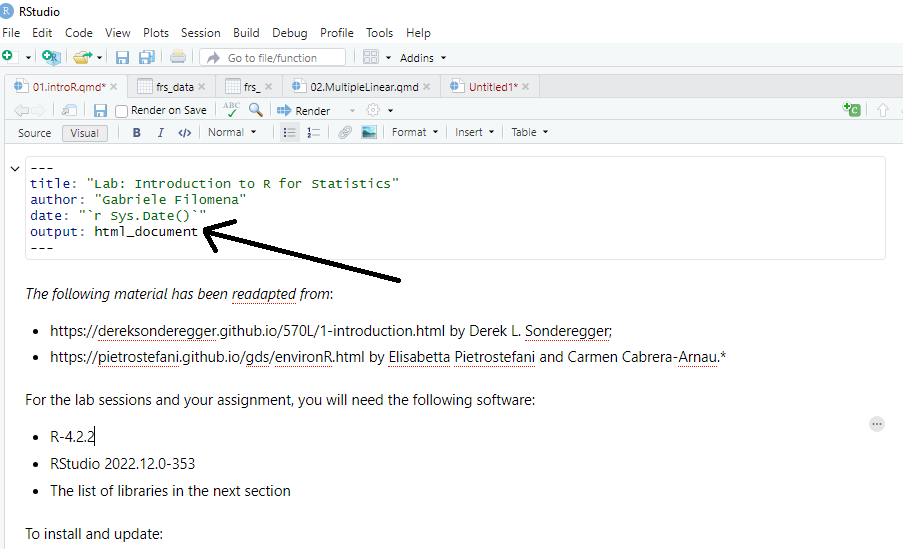
\includegraphics[width=3.01in,height=\textheight,keepaspectratio]{general/../img/quartoHeader.png}

\begin{verbatim}
    title: "Your Document Title"
    author: "Anonymous" # do not change
    format: pdf
\end{verbatim}

\begin{enumerate}
\def\labelenumi{\arabic{enumi}.}
\setcounter{enumi}{4}
\tightlist
\item
  Click the \textbf{Render} button in the RStudio toolbar (next to the
  Knit button).
\end{enumerate}

\bookmarksetup{startatroot}

\chapter*{Assessment Template}\label{assessment-template}
\addcontentsline{toc}{chapter}{Assessment Template}

\markboth{Assessment Template}{Assessment Template}

\textbf{Suggested Report Structure} --- This template follows the
requested sections. Each section contains guidance text and an empty R
code cell for your analysis. Download it from
\href{https://raw.githubusercontent.com/GDSL-UL/stats/main/general/reportTemplate.qmd}{here}and
work on it with your own Rstudio.

\section*{Setup}\label{setup}
\addcontentsline{toc}{section}{Setup}

\markright{Setup}

Load commonly used libraries for statistical analysis and data
manipulation.

\begin{Shaded}
\begin{Highlighting}[]
\CommentTok{\# Core tidyverse}
\FunctionTok{library}\NormalTok{(tidyverse)    }\CommentTok{\# includes ggplot2, dplyr, tidyr, readr, purrr, tibble, stringr, forcats}

\CommentTok{\# Tables \& reporting}
\FunctionTok{library}\NormalTok{(knitr)}
\FunctionTok{library}\NormalTok{(kableExtra)}

\CommentTok{\# Stats helpers}
\FunctionTok{library}\NormalTok{(broom)}

\DocumentationTok{\#\# These need to be installed on your PC.}
\end{Highlighting}
\end{Shaded}

\textbf{Once all the chunks execute correctly (no errors when running
all the code, \texttt{Ctrl\ +Alt\ +\ R} ) you can render the
\texttt{qmd} file. Follow the instructions
\href{https://gdsl-ul.github.io/stats/general/howSubmit.html}{here} to
render the document to a PDF. Remove this message and any irrelevant
text from the final submission.}

\begin{center}\rule{0.5\linewidth}{0.5pt}\end{center}

\section*{Introduction}\label{introduction}
\addcontentsline{toc}{section}{Introduction}

\markright{Introduction}

\textbf{Aim.} State clearly what you want to investigate (e.g.,
association between X and Y).\\
\textbf{Relevance.} Explain why the topic matters (theory, policy,
practice).\\
\textbf{Gap \& Research Question (RQ).} Identify what is missing in the
current knowledge and pose 1 RQ (avoid yes/no questions; ask \emph{how},
\emph{to what extent}, \emph{which factors}).\\
\textbf{Structure.} Briefly preview how the rest of the article is
organized.

\begin{center}\rule{0.5\linewidth}{0.5pt}\end{center}

\section*{Literature Review}\label{literature-review}
\addcontentsline{toc}{section}{Literature Review}

\markright{Literature Review}

\textbf{What we know.} Summarise key findings from prior studies
relevant to your RQ.\\
\textbf{Predictor rationale.} Justify the inclusion of variables
(theory-driven, prior empirical evidence).\\
\textbf{Remaining gap.} Specify precisely the gap this report addresses
(e.g., population, geography, time period, variable, method).\\
\emph{Note:} The goal is a clean, sensible analysis grounded in existing
ideas---not necessarily novel theory.

\begin{center}\rule{0.5\linewidth}{0.5pt}\end{center}

\section*{Methodology}\label{methodology}
\addcontentsline{toc}{section}{Methodology}

\markright{Methodology}

\textbf{Data.} Briefly describe the dataset (who collected it, when,
sample size, key variables).\\
\textbf{Transformations.} Describe any recoding/aggregation (e.g., bin
income into bands; reduce age groups from 11 to 3). Provide
justification.\\
\textbf{Techniques.} Outline and justify the statistical methods used
(e.g., GLM/LM, logistic regression, mixed models, matching).

Important: do not include statistics here, or graphs, or tables.

\section*{Results and Discussion}\label{results-and-discussion}
\addcontentsline{toc}{section}{Results and Discussion}

\markright{Results and Discussion}

\begin{Shaded}
\begin{Highlighting}[]
\CommentTok{\# summary variables, distribution, plots, etc}
\end{Highlighting}
\end{Shaded}

\textbf{Present the variables} Start with descriptive statistics for
your variables and distribution. If relevant, include discuss one-to-one
associations (briefly, e.g.~correlation plots). You can provide
correlation plots and/or boxplots but do not overload the report with
graphs.***

\begin{Shaded}
\begin{Highlighting}[]
\CommentTok{\# run the model, show tables summarising the Regression model.}
\end{Highlighting}
\end{Shaded}

\textbf{Results + interpretation.} Present estimates and interpret them
in plain language, tying back to the RQ. The Regression model should the
core of this section!! \textbf{Link to literature.} Compare/contrast
with prior findings. \textbf{Selective visuals.} Use clear charts/tables
to highlight key results only (avoid clutter).
------------------------------------------------------------------------

\section*{Conclusion}\label{conclusion}
\addcontentsline{toc}{section}{Conclusion}

\markright{Conclusion}

\textbf{Summary.} Recap the main findings vis‑à‑vis the RQs (do not
introduce new results).\\
\textbf{Limitations.} Offer a brief, honest self‑critique (data,
measurement, design, external validity).\\
\textbf{Implications.} Indicate what the findings suggest for practice,
policy, or future research.

\begin{center}\rule{0.5\linewidth}{0.5pt}\end{center}

\section*{}\label{section}
\addcontentsline{toc}{section}{}

\markright{}

\bookmarksetup{startatroot}

\chapter*{Working Directories and
Paths}\label{working-directories-and-paths}
\addcontentsline{toc}{chapter}{Working Directories and Paths}

\markboth{Working Directories and Paths}{Working Directories and Paths}

\section*{Start clean (optional but
handy)}\label{start-clean-optional-but-handy}
\addcontentsline{toc}{section}{Start clean (optional but handy)}

\markright{Start clean (optional but handy)}

\begin{Shaded}
\begin{Highlighting}[]
\CommentTok{\# Clear the environment (objects in memory)}
\FunctionTok{rm}\NormalTok{(}\AttributeTok{list =} \FunctionTok{ls}\NormalTok{())}
\end{Highlighting}
\end{Shaded}

\section*{Know where you are (working
directory)}\label{know-where-you-are-working-directory}
\addcontentsline{toc}{section}{Know where you are (working directory)}

\markright{Know where you are (working directory)}

Your working directory (WD) is the folder R uses as the starting point
for relative paths.

\begin{Shaded}
\begin{Highlighting}[]
\CommentTok{\# Show current working directory}
\FunctionTok{getwd}\NormalTok{()}
\end{Highlighting}
\end{Shaded}

\begin{verbatim}
[1] "C:/Users/ziye/Documents/GitHub/stats/general"
\end{verbatim}

A relative path is specified from the working directory (e.g.,
\texttt{data/myfile.csv}).

An absolute path starts at the drive root (e.g.,
\texttt{C:/Users/you/Documents/stats/data/myfile.csv}).

\section*{Recommended folder layout
(ENVS225)}\label{recommended-folder-layout-envs225}
\addcontentsline{toc}{section}{Recommended folder layout (ENVS225)}

\markright{Recommended folder layout (ENVS225)}

Download the module materials, unzip them them wherever you prefer. Then
un-nest the folder with the material (you will have one folder called
\texttt{stats-main} containing another folder inside, with the same
name. Aim for:

\begin{verbatim}
stats-main/
├── data/
├── labs_img/
└── labs/
\end{verbatim}

You can delete other sub-folders (e.g., docs) if you don't need them. It
is strongly advised to move this folder into your M: drive on university
machines, so it's accessible from every other PC on campus. Go to
\texttt{This\ PC} and access \texttt{M:\textbackslash{}(UoL\ userName)}

\section*{Set the working directory in RStudio (every time you use a new
PC)}\label{set-the-working-directory-in-rstudio-every-time-you-use-a-new-pc}
\addcontentsline{toc}{section}{Set the working directory in RStudio
(every time you use a new PC)}

\markright{Set the working directory in RStudio (every time you use a
new PC)}

Windows:
\texttt{RStudio\ \textgreater{}\ Tools\ \textgreater{}\ Global\ Options\ \textgreater{}\ General\ \textgreater{}\ Default\ working\ directory\ \textgreater{}}
Browse to your \texttt{stats-main} folder.

macOS:
\texttt{RStudio\ \textgreater{}\ Preferences\ \textgreater{}\ General}(older
versions: under \texttt{Appearance/Pane\ Layout)} set Default working
directory to \texttt{stats-main/}, this is the folder with all the
materials inside.

Then restart RStudio and verify:

\begin{Shaded}
\begin{Highlighting}[]
\FunctionTok{getwd}\NormalTok{()}
\end{Highlighting}
\end{Shaded}

\begin{verbatim}
[1] "C:/Users/ziye/Documents/GitHub/stats/general"
\end{verbatim}

\textbf{Tip}: In addition always save your projects inside the folder
\texttt{stats-main}. This keeps paths stable and prevents issues.

\section*{Loading data (CSV, Excel) with relative
paths}\label{loading-data-csv-excel-with-relative-paths}
\addcontentsline{toc}{section}{Loading data (CSV, Excel) with relative
paths}

\markright{Loading data (CSV, Excel) with relative paths}

\textbf{Option a) Your \texttt{.qmd} project is in \texttt{stats-main}}

\begin{Shaded}
\begin{Highlighting}[]
\FunctionTok{library}\NormalTok{(readr)}
\FunctionTok{library}\NormalTok{(readxl)}
\NormalTok{df }\OtherTok{\textless{}{-}} \FunctionTok{read\_csv}\NormalTok{(}\StringTok{"data/survey.csv"}\NormalTok{)}
\NormalTok{xls }\OtherTok{\textless{}{-}} \FunctionTok{read\_excel}\NormalTok{(}\StringTok{"data/survey.xlsx"}\NormalTok{, }\AttributeTok{sheet =} \DecValTok{1}\NormalTok{)}
\end{Highlighting}
\end{Shaded}

\textbf{Option b) Your \texttt{.qmd} project is in
\texttt{stats-main\textbackslash{}subfolder}}

\begin{Shaded}
\begin{Highlighting}[]
\NormalTok{df }\OtherTok{\textless{}{-}} \FunctionTok{read\_csv}\NormalTok{(}\StringTok{"../data/survey.csv"}\NormalTok{)}
\NormalTok{xls }\OtherTok{\textless{}{-}} \FunctionTok{read\_excel}\NormalTok{(}\StringTok{"../data/survey.xlsx"}\NormalTok{, }\AttributeTok{sheet =} \DecValTok{1}\NormalTok{)}
\end{Highlighting}
\end{Shaded}

In summary:

\begin{itemize}
\item
  \texttt{read\_csv(MyFile.csv)} RStudio looks in the working directory
  for the file \texttt{MyFile.csv}.
\item
  \texttt{read\_csv(MyFolder/MyFile.csv)} RStudio looks inside the
  Working Directory (WD), for the folder \texttt{MyFolder}, then the
  file \texttt{MyFile.csv}.
\item
  \texttt{read\_csv(data/survey.csv)} RStudio looks inside the WD, looks
  inside \texttt{data}, then \texttt{survey.csv}.
\item
  \texttt{read\_csv(\textasciigrave{}\textasciigrave{}../data/survey.csv}
  RStudio goes up one folder from the WD, then looks for the folder
  \texttt{data}and the file \texttt{surve.csv}.
\end{itemize}

You can always inspect where you are by

\begin{Shaded}
\begin{Highlighting}[]
\FunctionTok{getwd}\NormalTok{()}
\end{Highlighting}
\end{Shaded}

\begin{verbatim}
[1] "C:/Users/ziye/Documents/GitHub/stats/general"
\end{verbatim}

\begin{Shaded}
\begin{Highlighting}[]
\FunctionTok{list.files}\NormalTok{()        }\CommentTok{\# What’s in the working directory?}
\end{Highlighting}
\end{Shaded}

\begin{verbatim}
 [1] "about.qmd"           "assessment.html"     "assessment.qmd"     
 [4] "howSubmit.html"      "howSubmit.qmd"       "overview.html"      
 [7] "overview.qmd"        "reportTemplate.html" "reportTemplate.qmd" 
[10] "setup.qmd"           "wdPaths.html"        "wdPaths.qmd"        
[13] "wdPaths.rmarkdown"   "wdPaths_files"      
\end{verbatim}

\begin{Shaded}
\begin{Highlighting}[]
\FunctionTok{list.files}\NormalTok{(}\StringTok{"data"}\NormalTok{)  }\CommentTok{\# Do we see the data folder?}
\end{Highlighting}
\end{Shaded}

\begin{verbatim}
character(0)
\end{verbatim}

\bookmarksetup{startatroot}

\chapter{Lab: Introduction to R}\label{lab-introduction-to-r}

\emph{The following material has been readapted from}:

\begin{itemize}
\item
  https://dereksonderegger.github.io/570L/1-introduction.html by Derek
  L. Sonderegger;
\item
  For the lab sessions and your assignment, you will need the following
  software:
\item
  R-4.2.2 (or higher)
\item
  RStudio 2022.12.0-353 (or higher)
\item
  The list of libraries in the next section
\end{itemize}

To install and update:

\begin{itemize}
\tightlist
\item
  R, download the appropriate version from
  \href{https://cran.r-project.org/}{The Comprehensive R Archive Network
  (CRAN)}
\item
  RStudio, download the appropriate version from
  \href{https://posit.co/download/rstudio-desktop/}{Posit}
\end{itemize}

\section{R?}\label{r}

R is an open-source program that is commonly used in Statistics. It runs
on almost every platform and is completely free and is available at
\url{www.r-project.org}. Most of the cutting-edge statistical research
is first available on R.

R is a script based language, so there is no point and click interface.
While the initial learning curve will be steeper, understanding how to
write scripts will be valuable because it leaves a clear description of
what steps you performed in your data analysis. Typically you will want
to write a script in a separate file and then run individual lines. This
saves you from having to retype a bunch of commands and speeds up the
debugging process.

\section{R(Studio) Basics}\label{rstudio-basics}

We will be running R through the program RStudio which is located at
\href{http://www.rstudio.org}{rstudio.com}. When you first open up
RStudio the console window gives you some information about the version
of R you are running and then it gives the prompt
\texttt{\textgreater{}}. This prompt is waiting for you to input a
command. The prompt + tells you that the current command is spanning
multiple lines. In a script file you might have typed something like
this:

\begin{verbatim}
for( i in 1:5 ){
    print(i)
}
\end{verbatim}

Finding help about a certain function is very easy. At the prompt, just
type \texttt{help(function.name)} or \texttt{?function.name}. If you
don't know the name of the function, your best bet is to go the the web
page www.rseek.org which will search various R resources for your
keyword(s). Another great resource is the coding question and answer
site \href{http://stackoverflow.com}{stackoverflow}.

\subsection{Starting a session in
RStudio}\label{starting-a-session-in-rstudio}

Upon startup, RStudio will look something like this.

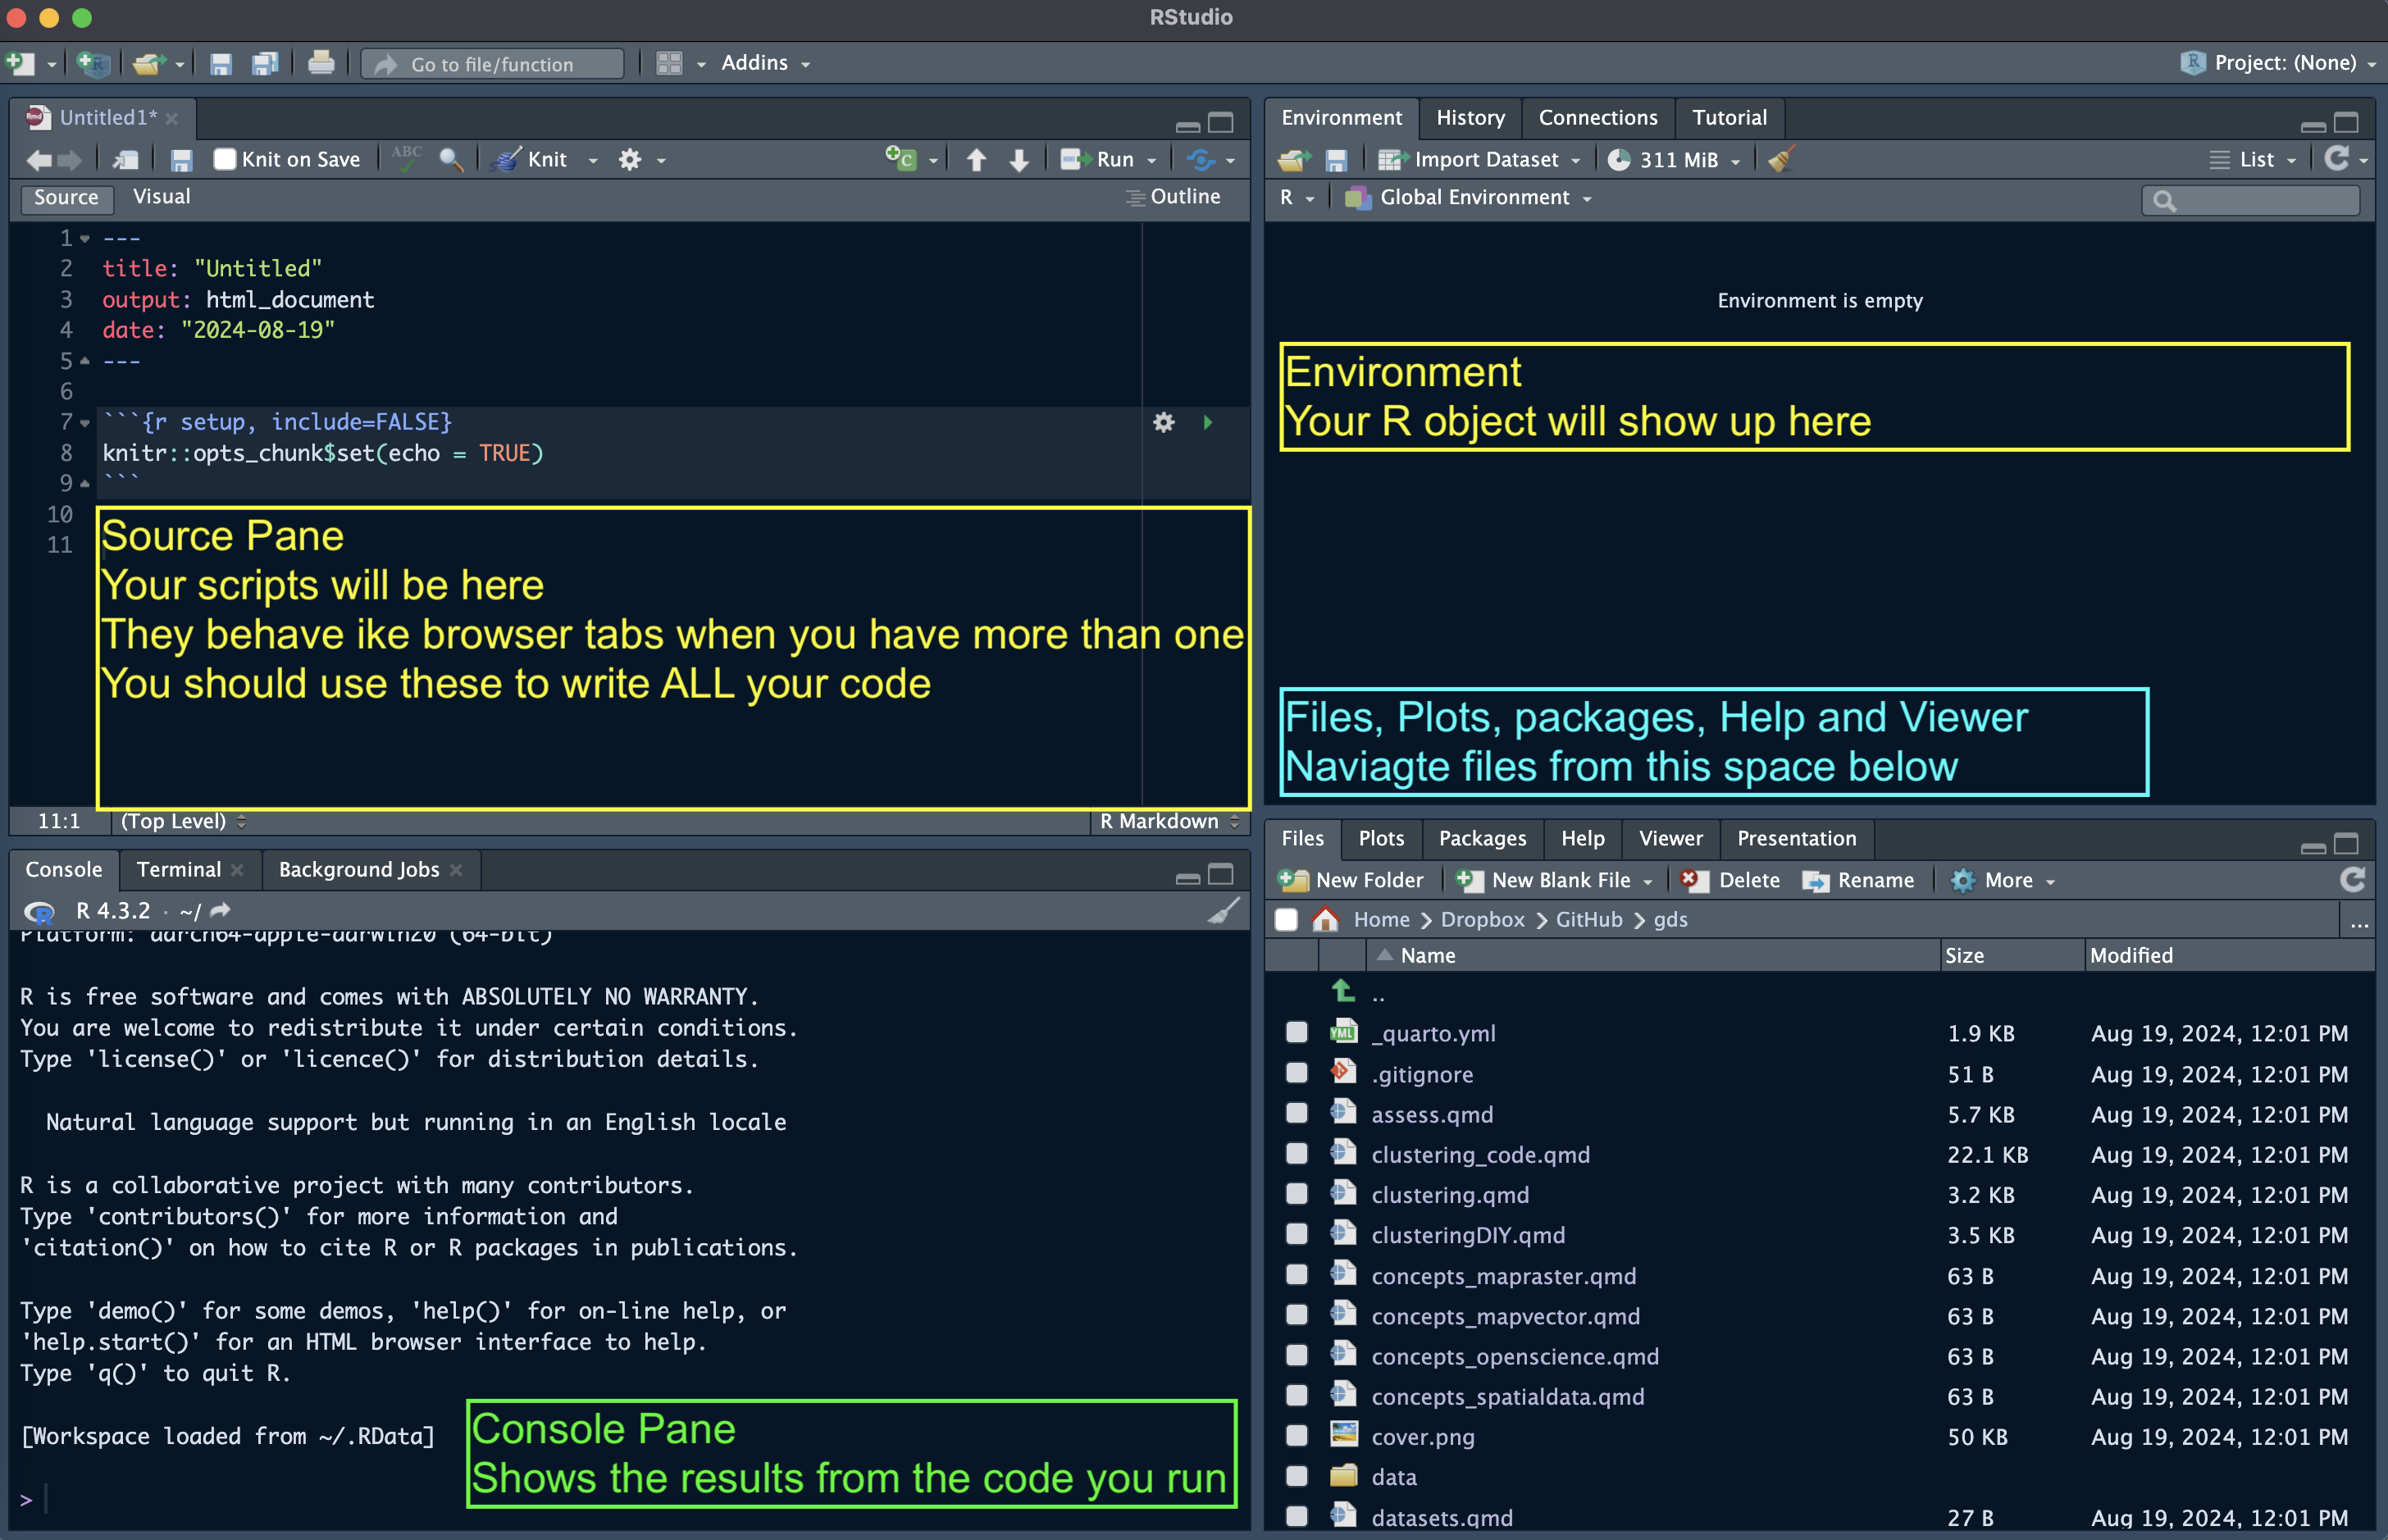
\includegraphics[width=9.71in,height=\textheight,keepaspectratio]{labs/../img/environ_R_1.png}

\emph{Note}: the \textbf{Pane Layout} and \textbf{Appearance} settings
can be altered:

\begin{itemize}
\tightlist
\item
  on Windows by clicking RStudio\textgreater Tools\textgreater Global
  Options\textgreater Appearance or Pane Layout
\item
  on Mac OS by clicking
  RStudio\textgreater Preferences\textgreater Appearance or Pane Layout.
\end{itemize}

You will also have a standard white background; but you can choose
specific
\href{https://quarto.org/docs/output-formats/html-themes.html}{themes}.

\textbf{Source Panel (Top-Left)}

This is where you write, edit, and view scripts, R Markdown/Quarto
documents, or R scripts. It allows:

\begin{itemize}
\tightlist
\item
  Editing Scripts: Write and edit R scripts or documents (\texttt{.R},
  \texttt{.Rmd}, \texttt{.qmd}).
\item
  Executing the Code: Run lines, blocks, or the entire script directly
  from the editor.
\end{itemize}

\textbf{Console Panel (Bottom-Left)}

\textbf{The Console is the main place to run R commands interactively.}
It allows:

\begin{itemize}
\tightlist
\item
  Executing the Code: Type and run R commands directly.
\item
  Viewing outputs, warnings, and errors for immediate feedback.
\item
  Browsing and reusing past commands (History Tab).
\item
  Toggling between the R Console, and the Terminal (yuo don't really
  need the latter).
\end{itemize}

\textbf{Environment Panel (Top-Right)}

This panel helps track variables, functions, and the history of commands
used. It contains:

\begin{itemize}
\tightlist
\item
  Environment Tab: Shows all current variables, datasets, and objects in
  your session, including their structure and values.
\item
  History Tab: Provides a record of past commands. You can re-run or
  move commands to the console or script.
\end{itemize}

\textbf{Files / Plots / Packages / Help Panel (Bottom-Right)}

This multifunctional panel is for file navigation, plotting, managing
packages, viewing help, and managing jobs. It contains:

\begin{itemize}
\tightlist
\item
  Files Tab: Navigate, open, and manage files and directories within
  your project.
\item
  Plots Tab: Displays plots generated in your session. You can export or
  navigate through multiple plots here.
\item
  Packages Tab: Lists installed packages and allows you to install,
  load, and update packages.
\item
  Help Tab: Displays help documentation for R functions, packages, and
  other resources. You can search for documentation by typing a function
  or package name.
\end{itemize}

At the start of a session, it's good practice clearing your R
environment (console):

\begin{Shaded}
\begin{Highlighting}[]
\FunctionTok{rm}\NormalTok{(}\AttributeTok{list =} \FunctionTok{ls}\NormalTok{())}
\end{Highlighting}
\end{Shaded}

In R, we are going to workin with \textbf{relative paths}. With the
command \texttt{getwd()}, you can see where your working directory is
currently set.

\begin{Shaded}
\begin{Highlighting}[]
\FunctionTok{getwd}\NormalTok{() }
\end{Highlighting}
\end{Shaded}

\subsection{Using the console}\label{using-the-console}

We can use the console to perform few operations. For example type in:

\begin{Shaded}
\begin{Highlighting}[]
\DecValTok{1}\SpecialCharTok{+}\DecValTok{1}
\end{Highlighting}
\end{Shaded}

\begin{verbatim}
[1] 2
\end{verbatim}

Slightly more complicated:

\begin{Shaded}
\begin{Highlighting}[]
\FunctionTok{print}\NormalTok{(}\StringTok{"hello world"}\NormalTok{)}
\end{Highlighting}
\end{Shaded}

\begin{verbatim}
[1] "hello world"
\end{verbatim}

If you are unsure about what a command does, use the ``Help'' panel in
your Files pane or type \texttt{?function} in the console. For example,
to see how the \texttt{dplyr::rename()} function works, type in
\texttt{?dplyr::rename}. When you see the double colon syntax like in
the previous command, it's a call to a package without loading its
library.

\subsection{R as a simple calculator}\label{r-as-a-simple-calculator}

You can use R as a simple calculator. At the prompt, type 2+3 and hit
enter. What you should see is the following

\begin{Shaded}
\begin{Highlighting}[]
\CommentTok{\# Some simple addition}
\DecValTok{2}\SpecialCharTok{+}\DecValTok{3}
\end{Highlighting}
\end{Shaded}

\begin{verbatim}
[1] 5
\end{verbatim}

In this fashion you can use R as a very capable calculator.

\begin{Shaded}
\begin{Highlighting}[]
\DecValTok{6}\SpecialCharTok{*}\DecValTok{8}
\end{Highlighting}
\end{Shaded}

\begin{verbatim}
[1] 48
\end{verbatim}

\begin{Shaded}
\begin{Highlighting}[]
\DecValTok{4}\SpecialCharTok{\^{}}\DecValTok{3}
\end{Highlighting}
\end{Shaded}

\begin{verbatim}
[1] 64
\end{verbatim}

\begin{Shaded}
\begin{Highlighting}[]
\FunctionTok{exp}\NormalTok{(}\DecValTok{1}\NormalTok{)   }\CommentTok{\# exp() is the exponential function}
\end{Highlighting}
\end{Shaded}

\begin{verbatim}
[1] 2.718282
\end{verbatim}

R has most constants and common mathematical functions you could ever
want. For example, the absolute value of a number is given by
\texttt{abs()}, and \texttt{round()} will round a value to the nearest
integer.

\begin{Shaded}
\begin{Highlighting}[]
\NormalTok{pi     }\CommentTok{\# the constant 3.14159265...}
\end{Highlighting}
\end{Shaded}

\begin{verbatim}
[1] 3.141593
\end{verbatim}

\begin{Shaded}
\begin{Highlighting}[]
\FunctionTok{abs}\NormalTok{(}\FloatTok{1.77}\NormalTok{) }
\end{Highlighting}
\end{Shaded}

\begin{verbatim}
[1] 1.77
\end{verbatim}

Whenever you call a function, there will be some arguments that are
mandatory, and some that are optional and the arguments are separated by
a comma. In the above statements the function \texttt{abs()} requires at
least one argument, and that is the number you want the absolute value
of.

When functions require more than one argument, arguments can be
specified via the order in which they are passed or by naming the
arguments. So for the \texttt{log()} function, for example, which
calculates the logarithm of a number, one can specify the arguments
using the named values; the order woudn't matter:

\begin{Shaded}
\begin{Highlighting}[]
\CommentTok{\# Demonstrating order does not matter if you specify}
\CommentTok{\# which argument is which}
\FunctionTok{log}\NormalTok{(}\AttributeTok{x=}\DecValTok{5}\NormalTok{, }\AttributeTok{base=}\DecValTok{10}\NormalTok{)   }
\end{Highlighting}
\end{Shaded}

\begin{verbatim}
[1] 0.69897
\end{verbatim}

\begin{Shaded}
\begin{Highlighting}[]
\FunctionTok{log}\NormalTok{(}\AttributeTok{base=}\DecValTok{10}\NormalTok{, }\AttributeTok{x=}\DecValTok{5}\NormalTok{)}
\end{Highlighting}
\end{Shaded}

\begin{verbatim}
[1] 0.69897
\end{verbatim}

When we don't specify which argument is which, R will decide that
\texttt{x} is the first argument, and \texttt{base} is the second.

\begin{Shaded}
\begin{Highlighting}[]
\CommentTok{\# If not specified, R will assume the second value is the base...}
\FunctionTok{log}\NormalTok{(}\DecValTok{5}\NormalTok{, }\DecValTok{10}\NormalTok{)}
\end{Highlighting}
\end{Shaded}

\begin{verbatim}
[1] 0.69897
\end{verbatim}

\begin{Shaded}
\begin{Highlighting}[]
\FunctionTok{log}\NormalTok{(}\DecValTok{10}\NormalTok{, }\DecValTok{5}\NormalTok{)}
\end{Highlighting}
\end{Shaded}

\begin{verbatim}
[1] 1.430677
\end{verbatim}

When we want to specify the arguments, we can do so using the
\texttt{name=value} notation.

\subsection{Variables Assignment}\label{variables-assignment}

We need to be able to assign a value to a variable to be able to use it
later. R does this by using an arrow \texttt{\textless{}-} or an equal
sign \texttt{=}. While R supports either, for readability, I suggest
people pick one assignment operator and stick with it.

\textbf{Variable names cannot start with a number, include spaces, and
they are case sensitive.}

\begin{Shaded}
\begin{Highlighting}[]
\NormalTok{var }\OtherTok{\textless{}{-}} \DecValTok{2}\SpecialCharTok{*}\FloatTok{7.5}       \CommentTok{\# create two variables}
\NormalTok{another\_var }\OtherTok{=} \DecValTok{5}   \CommentTok{\# notice they show up in \textquotesingle{}Environment\textquotesingle{} tab in RStudio!}
\NormalTok{var }
\end{Highlighting}
\end{Shaded}

\begin{verbatim}
[1] 15
\end{verbatim}

\begin{Shaded}
\begin{Highlighting}[]
\NormalTok{var }\SpecialCharTok{*}\NormalTok{ another\_var }
\end{Highlighting}
\end{Shaded}

\begin{verbatim}
[1] 75
\end{verbatim}

As your analysis gets more complicated, you'll want to save the results
to a variable so that you can access the results later. if you don't
assign the result to a variable, you have no way of accessing the
result.

\subsection{Working with Scripts}\label{working-with-scripts}

Normally you would use the Console for quick calculations or executions.
\textbf{In this module, though, we are going to work with Quarto
Markdown Scripts (\texttt{.qmd} files).}

The R Markdown is an implementation of the Markdown syntax that makes it
extremely easy to write webpages or scientific documents that include
code. This syntax was extended to allow users to embed R code directly
into more complex documents. Perhaps the easiest way to understand the
syntax is to look at an at the
\href{http://rmarkdown.rstudio.com}{RMarkdown website}. The R code in a
R Markdown document (\texttt{.rmd} file extension) can be nicely
separated from regular text using the three backticks (3 times `, see
below) and an instruction that it is R code that needs to be evaluated.
A code chunk will look like:

\begin{Shaded}
\begin{Highlighting}[]
    \ControlFlowTok{for}\NormalTok{ (i }\ControlFlowTok{in} \DecValTok{1}\SpecialCharTok{:}\DecValTok{5}\NormalTok{) \{}\FunctionTok{print}\NormalTok{(i)\}}
\end{Highlighting}
\end{Shaded}

\begin{verbatim}
[1] 1
[1] 2
[1] 3
[1] 4
[1] 5
\end{verbatim}

** \texttt{.qmd\ -\ the\ type\ of\ scripts\ we\ use\ -} are just a more
flexible development of \texttt{.rmd} files.**

Markdown files present several advantages compared to writing your code
in the console or just using scripts. You'll save yourself a huge amount
of work by embracing Markdown files from the beginning; you will keep
track of your code and your steps, be able to document and present how
you did your analysis (helpful when writing the methods section of a
paper), and it will make it easier to re-run an analysis after a change
in the data (such as additional data values, transformed data, or
removal of outliers) or once you spot an error. Finally, it makes the
script more readable.

\subsection{R Packages}\label{r-packages}

One of the greatest strengths about R is that so many people have
developed add-on packages to do some additional function. To download
and install the package from the Comprehensive R Archive Network (CRAN),
you just need to ask RStudio it to install it via the menu
\texttt{Tools} -\textgreater{} \texttt{Install\ Packages...}. Once
there, you just need to give the name of the package and RStudio will
download and install the package on your computer.

Once a package is downloaded and installed on your computer, it is
available, but it is not loaded into your current R session by default.
To improve overall performance only a few packages are loaded by default
and the you must explicitly load packages whenever you want to use them.
You only need to load them once per session/script.

\begin{Shaded}
\begin{Highlighting}[]
\FunctionTok{library}\NormalTok{(dplyr)   }\CommentTok{\# load the dplyr library, will be useful later}
\end{Highlighting}
\end{Shaded}

This is just a quick intro to R, now move to the actual practical of
week 1.

\bookmarksetup{startatroot}

\chapter{Lab: Exploring a Dataset}\label{lab-exploring-a-dataset}

\emph{The following material has been readapted from}:

\begin{itemize}
\tightlist
\item
  https://pietrostefani.github.io/gds/environR.html by Elisabetta
  Pietrostefani and Carmen Cabrera-Arnau
\item
  https://raw.githubusercontent.com/dereksonderegger/570L/master/07\_DataImport.Rmd
\end{itemize}

The lecture's slides can be found
\href{https://github.com/GDSL-UL/stats/blob/main/lectures/lecture01.pdf}{here}.

Before completing the practical, please take this
\href{https://canvas.liverpool.ac.uk/courses/84668/quizzes/168721}{quiz}.

For the lab sessions and your assignment, you will need the following
software:

\begin{itemize}
\tightlist
\item
  R-4.2.2 (or higher) \href{https://cran.r-project.org/}{The
  Comprehensive R Archive Network (CRAN)}
\item
  RStudio 2022.12.0-353 (or higher)
  \href{https://posit.co/download/rstudio-desktop/}{Posit}
\end{itemize}

\textbf{IMPORTANT: Before starting: verify that you have set the
directory correctly and familiarise yourself with working with
directories and loading files. These are the
\href{https://gdsl-ul.github.io/stats/general/wdPaths.html}{instructions}}.

\textbf{Now create a .qmd project. We use the
\texttt{File\ -\textgreater{}\ New\ File\ -\textgreater{}\ Quarto\ Document..}
dropdown option; a menu will appear asking you for the document title,
author, and preferred output type. You can select HTML. Call it
``\emph{week1}'' and save it in your main folder.}

Follow the practical below. You can describe what you are doing in
normal text. See
\href{https://quarto.org/docs/authoring/markdown-basics.html}{here} for
how to format normal text in Markdown documents

Remember, when you want to write code in a markdown document you have to
enclose it like this:

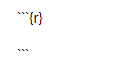
\includegraphics[width=0.39in,height=\textheight,keepaspectratio]{labs/../img/codeChunk.png}

\begin{quote}
or you can insert it manually:
\end{quote}

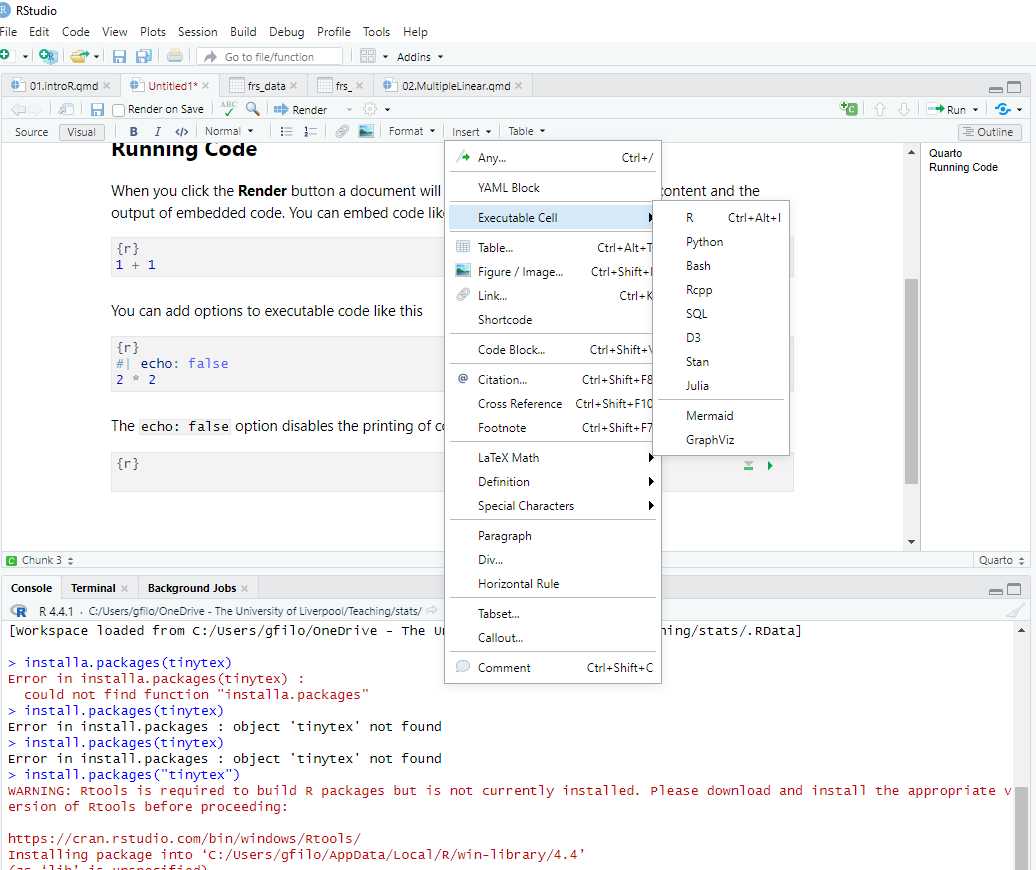
\includegraphics[width=3.45in,height=\textheight,keepaspectratio]{labs/../img/codeChunk_visual.png}

\section{Practice: Dataset and
Dataframes}\label{practice-dataset-and-dataframes}

Within this module we will be working with data stored in so-called
datasets. A dataset is a structured collection of data points that
represent various measurements or observations, often organized in a
tabular format with rows and columns. A dataset might contain
information about different locations, such as neighborhoods or cities,
with each row representing a place and each column detailing
characteristics like population density, average income, or number of
green parks. For example, a dataset could be compiled to study patterns
in urban mobility, where the data includes the number of daily
commuters, the distance they travel, and the mode of transport they use.
Datasets provide the essential building blocks for statistical analysis;
they enable exploring relationships, identifying patterns, and drawing
conclusions about certain phenomena.

Examples of everyday datasets:

\begin{itemize}
\tightlist
\item
  \textbf{Premier League Standings}: Each row represents a team, with
  columns for points, games played, wins, draws, and losses.
\item
  \textbf{Movie Dataset}: Each row represents a movie, with columns
  showing its title, genre, release year, director, and rating.
\item
  \textbf{Weather Dataset}: Each row shows a day's weather in a city,
  with columns for temperature, humidity, wind speed, and precipitation.
\end{itemize}

Usually, data is organized in

\begin{itemize}
\tightlist
\item
  \textbf{Columns} of data representing some trait or variable that we
  might be interested in. In general, we might wish to investigate the
  relationship between variables.
\item
  \textbf{Rows} represent a single object on which the column traits are
  measured.
\end{itemize}

For example, in a grade book for recording students scores throughout
the semester, their is one row for every student and columns for each
assignment. A greenhouse experiment dataset will have a row for every
plant and columns for treatment type and biomass.

\subsection{Datasets in R}\label{datasets-in-r}

In R, we want a way of storing data where it feels just as if we had an
Excel Spreadsheet where each row represents an observation and each
column represents some information about that observation. We will call
this object a \texttt{data.frame}, an R represention of a data set. The
easiest way to understand data frames is to create one.

\textbf{Task}: Copy the code below in your markdown. Create a
\texttt{data.frame} that represents an instructor's grade book, where
each row is a student, and each column represents some sort of
assessment.

\begin{Shaded}
\begin{Highlighting}[]
\FunctionTok{library}\NormalTok{(dplyr)}

\NormalTok{Grades }\OtherTok{\textless{}{-}} \FunctionTok{data.frame}\NormalTok{(}
  \AttributeTok{Name  =} \FunctionTok{c}\NormalTok{(}\StringTok{\textquotesingle{}Bob\textquotesingle{}}\NormalTok{,}\StringTok{\textquotesingle{}Jeff\textquotesingle{}}\NormalTok{,}\StringTok{\textquotesingle{}Mary\textquotesingle{}}\NormalTok{,}\StringTok{\textquotesingle{}Valerie\textquotesingle{}}\NormalTok{),     }
  \AttributeTok{Exam.1 =} \FunctionTok{c}\NormalTok{(}\DecValTok{90}\NormalTok{, }\DecValTok{75}\NormalTok{, }\DecValTok{92}\NormalTok{, }\DecValTok{85}\NormalTok{),}
  \AttributeTok{Exam.2 =} \FunctionTok{c}\NormalTok{(}\DecValTok{87}\NormalTok{, }\DecValTok{71}\NormalTok{, }\DecValTok{95}\NormalTok{, }\DecValTok{81}\NormalTok{)}
\NormalTok{)}
\CommentTok{\# Show the data.frame }
\CommentTok{\# View(Grades)  \# show the data in an Excel{-}like tab.  Doesn\textquotesingle{}t work when knitting }
\NormalTok{Grades          }\CommentTok{\# show the output in the console. This works when knitting}
\end{Highlighting}
\end{Shaded}

\begin{verbatim}
     Name Exam.1 Exam.2
1     Bob     90     87
2    Jeff     75     71
3    Mary     92     95
4 Valerie     85     81
\end{verbatim}

\textbf{To execute just one chunk of code press the green arrow
top-right of the chunk:}

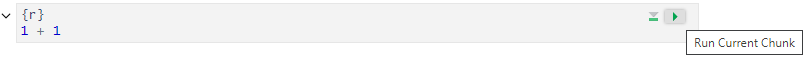
\includegraphics[width=2.68in,height=\textheight,keepaspectratio]{labs/../img/runChunk.png}

R allows two differnt was to access elements of the \texttt{data.frame}.
First is a matrix-like notation for accessing particular values.

\begin{longtable}[]{@{}ll@{}}
\toprule\noalign{}
Format & Result \\
\midrule\noalign{}
\endhead
\bottomrule\noalign{}
\endlastfoot
\texttt{{[}a,b{]}} & Element in row \texttt{a} and column \texttt{b} \\
\texttt{{[}a,{]}} & All of row \texttt{a} \\
\texttt{{[},b{]}} & All of column \texttt{b} \\
\end{longtable}

Because the columns have meaning and we have given them column names, it
is desirable to want to access an element by the name of the column as
opposed to the column number.

\textbf{Task}: Copy and Run:

\begin{Shaded}
\begin{Highlighting}[]
\NormalTok{Grades[, }\DecValTok{2}\NormalTok{]       }\CommentTok{\# print out all of column 2 }
\end{Highlighting}
\end{Shaded}

\begin{verbatim}
[1] 90 75 92 85
\end{verbatim}

\begin{Shaded}
\begin{Highlighting}[]
\NormalTok{Grades}\SpecialCharTok{$}\NormalTok{Name       }\CommentTok{\# The ${-}sign means to reference a column by its label}
\end{Highlighting}
\end{Shaded}

\begin{verbatim}
[1] "Bob"     "Jeff"    "Mary"    "Valerie"
\end{verbatim}

\subsection{Importing Data in R}\label{importing-data-in-r}

Usually we won't type the data in by hand, but rather load the data from
some package. Reading data from external sources is a necessary skill.

\textbf{\emph{Comma Separated Values}} \textbf{Data}

To consider how data might be stored, we first consider the simplest
file format: the comma separated values file (\texttt{.csv}). In this
file type, each of the ``cells'' of data are separated by a comma. For
example, the data file storing scores for three students might be as
follows:

\begin{verbatim}
Able, Dave, 98, 92, 94
Bowles, Jason, 85, 89, 91
Carr, Jasmine, 81, 96, 97
\end{verbatim}

Typically when you open up such a file on a computer with MS Excel
installed, Excel will open up the file assuming it is a spreadsheet and
put each element in its own cell. However, you can also open the file
using a more primitive program (say Notepad in Windows, TextEdit on a
Mac) you'll see the raw form of the data.

Having just the raw data without any sort of column header is
problematic (which of the three exams was the final??). Ideally we would
have column headers that store the name of the column.

\begin{verbatim}
LastName, FirstName, Exam1, Exam2, FinalExam
Able, Dave, 98, 92, 94
Bowles, Jason, 85, 89, 91
Carr, Jasmine, 81, 96, 97
\end{verbatim}

\textbf{Reading (\texttt{.csv}) files}

To make R read in the data arranged in this format, we need to tell R
three things:

\begin{enumerate}
\def\labelenumi{\arabic{enumi}.}
\item
  Where does the data live? Often this will be the name of a file on
  your computer, but the file could just as easily live on the internet
  (provided your computer has internet access).
\item
  Is the first row data or is it the column names?
\item
  What character separates the data? Some programs store data using tabs
  to distinguish between elements, some others use white space. R's
  mechanism for reading in data is flexible enough to allow you to
  specify what the separator is.
\end{enumerate}

The primary function that we'll use to read data from a file and into R
is the function \texttt{read.csv()}. This function has many optional
arguments but the most commonly used ones are outlined in the table
below.

\begin{longtable}[]{@{}
  >{\raggedright\arraybackslash}p{(\linewidth - 4\tabcolsep) * \real{0.3333}}
  >{\raggedright\arraybackslash}p{(\linewidth - 4\tabcolsep) * \real{0.3333}}
  >{\raggedright\arraybackslash}p{(\linewidth - 4\tabcolsep) * \real{0.3333}}@{}}
\toprule\noalign{}
\begin{minipage}[b]{\linewidth}\raggedright
Argument
\end{minipage} & \begin{minipage}[b]{\linewidth}\raggedright
Default
\end{minipage} & \begin{minipage}[b]{\linewidth}\raggedright
Description
\end{minipage} \\
\midrule\noalign{}
\endhead
\bottomrule\noalign{}
\endlastfoot
\texttt{file} & Required & A character string denoting the file
location. \\
\texttt{header} & \texttt{TRUE} & Specifies whether the first line
contains column headers. \\
\texttt{sep} & \texttt{","} & Specifies the character that separates
columns. For \texttt{read.csv()}, this is usually a comma. \\
\texttt{skip} & \texttt{0} & The number of lines to skip before reading
data; useful for files with descriptive text before the actual data. \\
\texttt{na.strings} & \texttt{"NA"} & Values that represent missing
data; multiple values can be specified, e.g.,
\texttt{c("NA",\ "-9999")}. \\
\texttt{quote} & \texttt{"} & Specifies the character used to quote
character strings, typically \texttt{"} or
\texttt{\textquotesingle{}}. \\
\texttt{stringsAsFactors} & \texttt{FALSE} & Controls whether character
strings are converted to factors; \texttt{FALSE} means they remain as
character data. \\
\texttt{row.names} & \texttt{NULL} & Allows specifying a column as row
names, or assigning \texttt{NULL} to use default indexing for rows. \\
\texttt{colClasses} & \texttt{NULL} & Specifies the data type for each
column to speed up reading for large files, e.g.,
\texttt{c("character",\ "numeric")}. \\
\texttt{encoding} & \texttt{"unknown"} & Sets the text encoding of the
file, which can be useful for files with special or international
characters. \\
\end{longtable}

Most of the time you just need to specify the file. \textbar{}

Task: Let's read in a dataset of terrorist attacks that have taken place
in the UK:

\begin{Shaded}
\begin{Highlighting}[]
\NormalTok{attacks }\OtherTok{\textless{}{-}} \FunctionTok{read.csv}\NormalTok{(}\AttributeTok{file   =} \StringTok{\textquotesingle{}../data/attacksUK.csv\textquotesingle{}}\NormalTok{)  }\CommentTok{\# where the data lives                                 }
\FunctionTok{View}\NormalTok{(attacks)}
\end{Highlighting}
\end{Shaded}

\section{Practice: Descriptive
Statistics}\label{practice-descriptive-statistics}

\subsection{Summarizing Data}\label{summarizing-data}

It is very important to be able to take a data set and produce summary
statistics such as the mean and standard deviation of a column. For this
sort of manipulation, we use the package \texttt{dplyr}. This package
allows chaining together many common actions to form a particular task.

The fundamental operations to perform on a data set are:

\begin{itemize}
\item
  \textbf{Subsetting} - Returns a dataframe with only particular columns
  or rows

  -- \texttt{select} - Selecting a subset of columns by name or column
  number.

  -- \texttt{filter} - Selecting a subset of rows from a data frame
  based on logical expressions.

  -- \texttt{slice} - Selecting a subset of rows by row number.
\item
  \texttt{arrange} - Re-ordering the rows of a data frame.
\item
  \texttt{mutate} - Add a new column that is some function of other
  columns.
\item
  \texttt{summarise} - calculate some summary statistic of a column of
  data. This collapses a set of rows into a single row.
\end{itemize}

Each of these operations is a function in the package \texttt{dplyr}.
These functions all have a similar calling syntax:

\begin{itemize}
\item
  The first argument is a data set.
\item
  Subsequent arguments describe what to do with the input data frame and
  you can refer to the columns without using the \texttt{df\$column}
  notation.
\end{itemize}

All of these functions will return a data set.

Let's consider the \texttt{summarize} function to calculate the mean
score for \texttt{Exam.1}. Notice that this takes a data frame of four
rows, and summarizes it down to just one row that represents the
summarized data for all four students.

\begin{Shaded}
\begin{Highlighting}[]
\FunctionTok{library}\NormalTok{(dplyr) }\CommentTok{\# load the library}
\NormalTok{Grades }\SpecialCharTok{\%\textgreater{}\%}
  \FunctionTok{summarize}\NormalTok{( }\AttributeTok{Exam.1.mean =} \FunctionTok{mean}\NormalTok{( Exam}\FloatTok{.1}\NormalTok{ ) )}
\end{Highlighting}
\end{Shaded}

\begin{verbatim}
  Exam.1.mean
1        85.5
\end{verbatim}

Similarly you could calculate the \textbf{standard deviation} for the
exam as well.

\begin{Shaded}
\begin{Highlighting}[]
\NormalTok{Grades }\SpecialCharTok{\%\textgreater{}\%}
  \FunctionTok{summarize}\NormalTok{( }\AttributeTok{Exam.1.mean =} \FunctionTok{mean}\NormalTok{( Exam}\FloatTok{.1}\NormalTok{ ),}
             \AttributeTok{Exam.1.sd   =} \FunctionTok{sd}\NormalTok{(   Exam}\FloatTok{.1}\NormalTok{   ) )}
\end{Highlighting}
\end{Shaded}

\begin{verbatim}
  Exam.1.mean Exam.1.sd
1        85.5  7.593857
\end{verbatim}

\textbf{Task:} Write the code above in your markdown file and run it. Do
not to copy it this time.

The \texttt{\%\textgreater{}\%} operator works by translating the
command \texttt{a\ \%\textgreater{}\%\ f(b)} to the expression
\texttt{f(a,b)}. This operator works on any function \texttt{f}. This is
useful when we want to start with \texttt{x}, and first apply a function
\texttt{f()}, then \texttt{g()}, and then \texttt{h()}; the usual R
command would be \texttt{h(g(f(x)))} which is hard to read. Using the
pipe command \texttt{\%\textgreater{}\%}, this sequence of operations
becomes
\texttt{x\ \%\textgreater{}\%\ f()\ \%\textgreater{}\%\ g()\ \%\textgreater{}\%\ h()}.

Below, the code takes the Grades dataframe and calculates a column for
the average exam score, and then sorts the data according to the that
average score

\begin{Shaded}
\begin{Highlighting}[]
\NormalTok{Grades }\SpecialCharTok{\%\textgreater{}\%}   \FunctionTok{mutate}\NormalTok{( }\AttributeTok{Avg.Score =}\NormalTok{ (Exam}\FloatTok{.1} \SpecialCharTok{+}\NormalTok{ Exam}\FloatTok{.2}\NormalTok{) }\SpecialCharTok{/} \DecValTok{2}\NormalTok{ ) }\SpecialCharTok{\%\textgreater{}\%}   \FunctionTok{arrange}\NormalTok{( Avg.Score )}
\end{Highlighting}
\end{Shaded}

\begin{verbatim}
     Name Exam.1 Exam.2 Avg.Score
1    Jeff     75     71      73.0
2 Valerie     85     81      83.0
3     Bob     90     87      88.5
4    Mary     92     95      93.5
\end{verbatim}

You don't have to memorise this.

Let's go back to the terrorist attacks dataframe. There are attacks
perpetrated by several different groups. Each record is a single attack
and contains information about who perpetrated the attack, what year,
how many were killed and how many were wounded. You can get a glimpse of
the dataframe with the function head

\begin{Shaded}
\begin{Highlighting}[]
\FunctionTok{head}\NormalTok{(attacks, }\AttributeTok{n =} \DecValTok{10}\NormalTok{)}
\end{Highlighting}
\end{Shaded}

\begin{verbatim}
   nrKilled nrWound year        country                        group
1         0       0 2005 United Kingdom   Abu Hafs al-Masri Brigades
2         0       0 2005 United Kingdom   Abu Hafs al-Masri Brigades
3         0       0 2005 United Kingdom   Abu Hafs al-Masri Brigades
4         0       0 2005 United Kingdom   Abu Hafs al-Masri Brigades
5         0       1 1982 United Kingdom Abu Nidal Organization (ANO)
6         0       0 2014 United Kingdom                   Anarchists
7         0       0 2014 United Kingdom                   Anarchists
8         0       0 2014 United Kingdom                   Anarchists
9         0       0 2014 United Kingdom                   Anarchists
10        0       0 2014 United Kingdom                   Anarchists
                           attack                      target
1               Bombing/Explosion              Transportation
2               Bombing/Explosion              Transportation
3               Bombing/Explosion              Transportation
4               Bombing/Explosion              Transportation
5                   Assassination     Government (Diplomatic)
6  Facility/Infrastructure Attack                    Business
7  Facility/Infrastructure Attack                    Business
8  Facility/Infrastructure Attack                    Business
9  Facility/Infrastructure Attack Private Citizens & Property
10 Facility/Infrastructure Attack                      Police
                      weapon
1  Explosives/Bombs/Dynamite
2  Explosives/Bombs/Dynamite
3  Explosives/Bombs/Dynamite
4  Explosives/Bombs/Dynamite
5                   Firearms
6                 Incendiary
7                 Incendiary
8                 Incendiary
9                 Incendiary
10                Incendiary
\end{verbatim}

We might want to compare different actors and see the mean and standard
deviation of the number of people wound, by each group's attack, across
time. To do this, we are still going to use the \texttt{summarize}, but
we will precede that with \texttt{group\_by(group)} to tell the
subsequent \texttt{dplyr} functions to perform the actions separately
for each breed.

\begin{Shaded}
\begin{Highlighting}[]
\NormalTok{attacks }\SpecialCharTok{\%\textgreater{}\%}
  \FunctionTok{group\_by}\NormalTok{( group) }\SpecialCharTok{\%\textgreater{}\%}
  \FunctionTok{summarise}\NormalTok{( }\AttributeTok{Mean =} \FunctionTok{mean}\NormalTok{(attacks}\SpecialCharTok{$}\NormalTok{nrWound), }
             \AttributeTok{Std.Dev =} \FunctionTok{sd}\NormalTok{(attacks}\SpecialCharTok{$}\NormalTok{nrWound))}
\end{Highlighting}
\end{Shaded}

\begin{verbatim}
# A tibble: 38 x 3
   group                                               Mean Std.Dev
   <chr>                                              <dbl>   <dbl>
 1 Abu Hafs al-Masri Brigades                         0.963    7.22
 2 Abu Nidal Organization (ANO)                       0.963    7.22
 3 Anarchists                                         0.963    7.22
 4 Animal Liberation Front (ALF)                      0.963    7.22
 5 Animal Rights Activists                            0.963    7.22
 6 Armenian Secret Army for the Liberation of Armenia 0.963    7.22
 7 Black September                                    0.963    7.22
 8 Continuity Irish Republican Army (CIRA)            0.963    7.22
 9 Dissident Republicans                              0.963    7.22
10 Informal Anarchist Federation                      0.963    7.22
# i 28 more rows
\end{verbatim}

\textbf{Task:} Write the code above in your markdown file and run it.
Try out another categorical variable instead of \texttt{group}
(e.g.~\texttt{year}) and \texttt{nrKilled} instead of \texttt{nrWound}.

Let's now move to another dataset to address a research question.

For illustration purposes, we will use the \textbf{Family Resources
Survey (FRS)}. The FRS is an annual survey conducted by the UK
government that collects detailed information about the income, living
conditions, and resources of private households across the United
Kingdom. Managed by the Department for Work and Pensions (DWP), the FRS
provides data that is essential for understanding the economic and
social conditions of households and informing public policy.

Consider questions such as:

\begin{itemize}
\tightlist
\item
  How many respondents (persons) are there in the 2016-17 FRS?
\item
  How many variables (population attributes) are there?
\item
  What types of variables are present in the FRS?
\item
  What is the most detailed geography available in the FRS?
\end{itemize}

\textbf{Task}: To answer these questions,
\href{https://canvas.liverpool.ac.uk/courses/84668/files/12887864?wrap=1}{download}
from Canvas, save in the data folder, load and inspect the dataset.

\begin{Shaded}
\begin{Highlighting}[]
\CommentTok{\# the FRS dataset should be already loaded, otherwise}
\NormalTok{frs\_data }\OtherTok{\textless{}{-}} \FunctionTok{read.csv}\NormalTok{(}\StringTok{"../data/FRS/FRS16{-}17\_labels.csv"}\NormalTok{) }

\CommentTok{\# Display basic structure }
\FunctionTok{glimpse}\NormalTok{(frs\_data)}
\end{Highlighting}
\end{Shaded}

\begin{verbatim}
Rows: 44,145
Columns: 45
$ household        <int> 6087, 6101, 6103, 6122, 6134, 6136, 6138, 6140, 6143,~
$ family           <int> 1, 1, 1, 1, 1, 1, 1, 1, 1, 1, 1, 1, 1, 1, 1, 1, 1, 1,~
$ person           <int> 5, 3, 3, 3, 2, 4, 4, 3, 3, 4, 4, 3, 4, 2, 5, 3, 4, 3,~
$ country          <chr> "England", "England", "England", "Northern Ireland", ~
$ region           <chr> "London", "South East", "Yorks and the Humber", "Nort~
$ age_group        <chr> "05-10", "05-10", "05-10", "05-10", "05-10", "05-10",~
$ sex              <chr> "Female", "Male", "Male", "Female", "Female", "Female~
$ marital_status   <chr> "Single", "Single", "Single", "Single", "Single", "Si~
$ ethnicity        <chr> "Mixed / multiple ethnic groups", "White", "White", "~
$ hrp              <chr> "Not HRP", "Not HRP", "Not HRP", "Not HRP", "Not HRP"~
$ rel_to_hrp       <chr> "Son/daughter (incl. adopted)", "Son/daughter (incl. ~
$ lifestage        <chr> "Child (0-17)", "Child (0-17)", "Child (0-17)", "Chil~
$ dependent        <chr> "Dependent", "Dependent", "Dependent", "Dependent", "~
$ arrival_year     <chr> "UK Born", "UK Born", "UK Born", "UK Born", "UK Born"~
$ birth_country    <chr> "Dependent child", "Dependent child", "Dependent chil~
$ care_hours       <chr> "0 hours per week", "0 hours per week", "0 hours per ~
$ educ_age         <chr> "Dependent child", "Dependent child", "Dependent chil~
$ educ_type        <chr> "School (full-time)", "School (full-time)", "School (~
$ fam_youngest     <chr> "7", "4", "0", "7", "0", "9", "10", "0", "3", "10", "~
$ fam_toddlers     <int> 0, 1, 1, 0, 2, 0, 0, 2, 1, 0, 0, 1, 0, 1, 0, 0, 0, 1,~
$ fam_size         <int> 4, 4, 4, 3, 4, 4, 3, 5, 4, 4, 3, 4, 4, 3, 5, 4, 4, 4,~
$ happy            <chr> "Dependent child", "Dependent child", "Dependent chil~
$ health           <chr> "Not known", "Not known", "Not known", "Not known", "~
$ hh_accom_type    <chr> "Terraced house/bungalow", "Detached house/bungalow",~
$ hh_benefits      <int> 10868, 0, 1768, 8632, 8372, 1768, 1768, 1768, 0, 0, 1~
$ hh_composition   <chr> "Three or more adults, 1+ children", "One adult femal~
$ hh_ctax_band     <chr> "Band D", "Band F", "Band A", "Band B", "Band A", "Ba~
$ hh_housing_costs <chr> "4316", "10296", "5408", "Northern Ireland", "5720", ~
$ hh_income_gross  <int> 54236, 180804, 26936, 19968, 17992, 76596, 31564, 366~
$ hh_income_net    <int> 44668, 120640, 23556, 19968, 17992, 62868, 29744, 287~
$ hh_size          <int> 5, 4, 4, 3, 4, 4, 4, 5, 4, 4, 4, 4, 4, 5, 5, 4, 4, 4,~
$ hh_tenure        <chr> "Mortgaged (including part rent / part own)", "Mortga~
$ highest_qual     <chr> "Dependent child", "Dependent child", "Dependent chil~
$ income_gross     <int> 0, 0, 0, 0, 0, 0, 0, 0, 0, 0, 0, 0, 0, 0, 0, 0, 0, 0,~
$ income_net       <int> 0, 0, 0, 0, 0, 0, 0, 0, 0, 0, 0, 0, 0, 0, 0, 0, 0, 0,~
$ jobs             <chr> "Dependent child", "Dependent child", "Dependent chil~
$ life_satisf      <chr> "Dependent child", "Dependent child", "Dependent chil~
$ nssec            <chr> "Dependent child", "Dependent child", "Dependent chil~
$ sic_chapter      <chr> "Dependent child", "Dependent child", "Dependent chil~
$ sic_division     <chr> "Dependent child", "Dependent child", "Dependent chil~
$ soc2010          <chr> "Dependent child", "Dependent child", "Dependent chil~
$ work_hours       <chr> "Dependent child", "Dependent child", "Dependent chil~
$ workstatus       <chr> "Dependent Child", "Dependent Child", "Dependent Chil~
$ years_ft_work    <chr> "Dependent child", "Dependent child", "Dependent chil~
$ survey_weight    <int> 2315, 1317, 2449, 427, 1017, 1753, 1363, 1344, 828, 1~
\end{verbatim}

and summary:

\begin{Shaded}
\begin{Highlighting}[]
\FunctionTok{summary}\NormalTok{(frs\_data)}
\end{Highlighting}
\end{Shaded}

\begin{verbatim}
   household         family          person       country         
 Min.   :    1   Min.   :1.000   Min.   :1.00   Length:44145      
 1st Qu.: 4816   1st Qu.:1.000   1st Qu.:1.00   Class :character  
 Median : 9673   Median :1.000   Median :2.00   Mode  :character  
 Mean   : 9677   Mean   :1.106   Mean   :1.98                     
 3rd Qu.:14553   3rd Qu.:1.000   3rd Qu.:3.00                     
 Max.   :19380   Max.   :6.000   Max.   :9.00                     
    region           age_group             sex            marital_status    
 Length:44145       Length:44145       Length:44145       Length:44145      
 Class :character   Class :character   Class :character   Class :character  
 Mode  :character   Mode  :character   Mode  :character   Mode  :character  
                                                                            
                                                                            
                                                                            
  ethnicity             hrp             rel_to_hrp         lifestage        
 Length:44145       Length:44145       Length:44145       Length:44145      
 Class :character   Class :character   Class :character   Class :character  
 Mode  :character   Mode  :character   Mode  :character   Mode  :character  
                                                                            
                                                                            
                                                                            
  dependent         arrival_year       birth_country       care_hours       
 Length:44145       Length:44145       Length:44145       Length:44145      
 Class :character   Class :character   Class :character   Class :character  
 Mode  :character   Mode  :character   Mode  :character   Mode  :character  
                                                                            
                                                                            
                                                                            
   educ_age          educ_type         fam_youngest        fam_toddlers   
 Length:44145       Length:44145       Length:44145       Min.   :0.0000  
 Class :character   Class :character   Class :character   1st Qu.:0.0000  
 Mode  :character   Mode  :character   Mode  :character   Median :0.0000  
                                                          Mean   :0.2557  
                                                          3rd Qu.:0.0000  
                                                          Max.   :4.0000  
    fam_size        happy              health          hh_accom_type     
 Min.   :1.000   Length:44145       Length:44145       Length:44145      
 1st Qu.:2.000   Class :character   Class :character   Class :character  
 Median :2.000   Mode  :character   Mode  :character   Mode  :character  
 Mean   :2.599                                                           
 3rd Qu.:4.000                                                           
 Max.   :9.000                                                           
  hh_benefits    hh_composition     hh_ctax_band       hh_housing_costs  
 Min.   :    0   Length:44145       Length:44145       Length:44145      
 1st Qu.:    0   Class :character   Class :character   Class :character  
 Median : 1768   Mode  :character   Mode  :character   Mode  :character  
 Mean   : 5670                                                           
 3rd Qu.:10192                                                           
 Max.   :54080                                                           
 hh_income_gross   hh_income_net        hh_size      hh_tenure        
 Min.   :-326092   Min.   :-334776   Min.   :1.00   Length:44145      
 1st Qu.:  22256   1st Qu.:  20748   1st Qu.:2.00   Class :character  
 Median :  35984   Median :  31512   Median :3.00   Mode  :character  
 Mean   :  46076   Mean   :  37447   Mean   :2.96                     
 3rd Qu.:  57252   3rd Qu.:  47008   3rd Qu.:4.00                     
 Max.   :1165216   Max.   :1116596   Max.   :9.00                     
 highest_qual        income_gross       income_net          jobs          
 Length:44145       Min.   :-354848   Min.   :-358592   Length:44145      
 Class :character   1st Qu.:     52   1st Qu.:      0   Class :character  
 Mode  :character   Median :  12740   Median :  12012   Mode  :character  
                    Mean   :  17305   Mean   :  14204                     
                    3rd Qu.:  23712   3rd Qu.:  20384                     
                    Max.   :1127360   Max.   :1110928                     
 life_satisf           nssec           sic_chapter        sic_division      
 Length:44145       Length:44145       Length:44145       Length:44145      
 Class :character   Class :character   Class :character   Class :character  
 Mode  :character   Mode  :character   Mode  :character   Mode  :character  
                                                                            
                                                                            
                                                                            
   soc2010           work_hours         workstatus        years_ft_work     
 Length:44145       Length:44145       Length:44145       Length:44145      
 Class :character   Class :character   Class :character   Class :character  
 Mode  :character   Mode  :character   Mode  :character   Mode  :character  
                                                                            
                                                                            
                                                                            
 survey_weight  
 Min.   :  221  
 1st Qu.: 1097  
 Median : 1380  
 Mean   : 1459  
 3rd Qu.: 1742  
 Max.   :39675  
\end{verbatim}

\subsection{Understanding the Structure of the FRS
Datafile}\label{understanding-the-structure-of-the-frs-datafile}

In the FRS data structure, each row represents a person, but:

\begin{itemize}
\tightlist
\item
  Each person is nested within a family.
\item
  Each family is nested within a household.
\end{itemize}

Below is an example dataset structure:

\begin{longtable}[]{@{}
  >{\raggedright\arraybackslash}p{(\linewidth - 14\tabcolsep) * \real{0.1250}}
  >{\raggedright\arraybackslash}p{(\linewidth - 14\tabcolsep) * \real{0.1250}}
  >{\raggedright\arraybackslash}p{(\linewidth - 14\tabcolsep) * \real{0.1250}}
  >{\raggedright\arraybackslash}p{(\linewidth - 14\tabcolsep) * \real{0.1250}}
  >{\raggedright\arraybackslash}p{(\linewidth - 14\tabcolsep) * \real{0.1250}}
  >{\raggedright\arraybackslash}p{(\linewidth - 14\tabcolsep) * \real{0.1250}}
  >{\raggedright\arraybackslash}p{(\linewidth - 14\tabcolsep) * \real{0.1250}}
  >{\raggedright\arraybackslash}p{(\linewidth - 14\tabcolsep) * \real{0.1250}}@{}}
\toprule\noalign{}
\begin{minipage}[b]{\linewidth}\raggedright
household
\end{minipage} & \begin{minipage}[b]{\linewidth}\raggedright
family
\end{minipage} & \begin{minipage}[b]{\linewidth}\raggedright
person
\end{minipage} & \begin{minipage}[b]{\linewidth}\raggedright
region
\end{minipage} & \begin{minipage}[b]{\linewidth}\raggedright
age\_group
\end{minipage} & \begin{minipage}[b]{\linewidth}\raggedright
sex
\end{minipage} & \begin{minipage}[b]{\linewidth}\raggedright
marital\_status
\end{minipage} & \begin{minipage}[b]{\linewidth}\raggedright
rel\_to\_hrp
\end{minipage} \\
\midrule\noalign{}
\endhead
\bottomrule\noalign{}
\endlastfoot
1 & 1 & 1 & London & 40-44 & Female & Married/Civil partnership &
Spouse \\
1 & 1 & 2 & London & 40-44 & Male & Married/Civil partnership &
Household Representative \\
1 & 1 & 3 & London & 5-10 & Male & Single & Son/daughter
(incl.~adopted) \\
1 & 1 & 4 & London & 5-10 & Female & Single & Son/daughter
(incl.~adopted) \\
1 & 1 & 5 & London & 16-19 & Male & Single & Step-son/daughter \\
2 & 1 & 1 & Scotland & 35-39 & Male & Single & Household
Representative \\
3 & 1 & 1 & Yorks and the Humber & 35-39 & Female & Married/Civil
partnership & Household Representative \\
3 & 1 & 2 & Yorks and the Humber & 35-39 & Male & Married/Civil
partnership & Spouse \\
3 & 1 & 3 & Yorks and the Humber & 5-10 & Male & Single &
Step-son/daughter \\
4 & 1 & 1 & Wales & 0-4 & Male & Single & Son/daughter
(incl.~adopted) \\
4 & 1 & 2 & Wales & 60-64 & Male & Married/Civil partnership & Household
Representative \\
4 & 1 & 3 & Wales & 55-59 & Female & Married/Civil partnership &
Spouse \\
4 & 2 & 3 & Wales & 30-34 & Female & Single & Son/daughter
(incl.~adopted) \\
\end{longtable}

The first five people in the FRS all belong to the same household
(household 1); they also all belong to the same family. This family
comprises a married middle-aged couple plus their three children, one of
whom is a stepson.

The second household (household 2) comprises only one person -- a single
middle-aged male.The third household comprises another married couple,
this time with two children.

Superficially the fourth household looks similar to households 1 and 2:
a married couple plus their daughter. The difference is that this
particular married couple is nearing retirement age, and their daughter
is middle-aged. Consequently, despite being a child of the married
couple, the middle-aged daughter is treated as a separate `family'
(family 2 in the household). This is because the FRS (and Census) define
a `family' as a couple plus any `dependent' children. A dependent child
is defined as a child who is either` aged 0-15 or aged 16-19, unmarried
and in full-time education. All children aged 16-19 who are married or
no longer in full-time education are regarded as `independent' adults
who form their own family unit, as are all children aged 20+.

The inclusion of all persons in a household allows us more flexibility
in the types of research question we can answer. For example, we could
explore how the likelihood of a woman being in paid employment
\texttt{WorkStatus} is influenced by the age of the youngest child still
living in her family (if any) \texttt{fam\_youngest}.

In the FRS (and Census), a ``family'' is defined as a couple and any
``dependent'' children. Dependent children are defined as those aged
0--15, or aged 16--19 if unmarried and in full-time education.

\subsection{Explore the Distribution of Your Outcome
Variable}\label{explore-the-distribution-of-your-outcome-variable}

Before starting your analysis, it is critical to know the type of scale
used to measure your outcome variable: is it categorical or continuous?
Here we will start off by exploring a continuous variable which can then
turn into a categorical variable (e.g.~top earners: yes or no). We
explore the income distribution in the UK by first looking at the low
and high end of the distribution ie. What sorts of people have high (or
low) incomes?

In the FRS each person's annual income is recorded, both gross (pre-tax)
and net (post-tax). This income includes all income sources, including
earnings, profits, investment returns, state benefits, occupational
pensions etc. As it is possible to make a loss on some of these
activities, it is also possible (although unusual) for someone's gross
or net annual income in a given year to be negative (representing an
overall loss).

\textbf{Task}: Load the FRS dataset into your R environment, if it's not
already loaded, and inspect the data.

Open the dataset in RStudio's \textbf{Data Viewer} to explore its
structure, including the \texttt{income\_gross} and \texttt{income\_net}
variables.

\begin{Shaded}
\begin{Highlighting}[]
 \CommentTok{\# Open the data in the RStudio Viewer}
\FunctionTok{View}\NormalTok{(frs\_data)}
\end{Highlighting}
\end{Shaded}

in the \textbf{Data Viewer} tab, scroll horizontally to locate the
\texttt{income\_gross} and \texttt{income\_net} columns. If columns are
listed alphabetically, they will appear near other attributes that start
with ``income.''

You should notice two things:

\begin{itemize}
\tightlist
\item
  Incomes are recorded to the nearest £, NOT in income bands.
\item
  Dependent children almost all have a recorded income of £0.
\end{itemize}

This second observation highlights the somewhat loose wording of our
question above (\emph{What sorts of people have high (or low)
incomes?}). To avoid reaching the somewhat banal conclusion that those
with the lowest of all incomes are almost all children, we should
re-frame the question more precisely as \emph{What sorts of people
(excluding dependent children) have low incomes?}

\textbf{Task}: Determine the Scale of the Outcome Variable.

\begin{Shaded}
\begin{Highlighting}[]
\CommentTok{\# Summarize income variables}
\FunctionTok{summary}\NormalTok{(frs\_data}\SpecialCharTok{$}\NormalTok{income\_gross)}
\end{Highlighting}
\end{Shaded}

\begin{verbatim}
   Min. 1st Qu.  Median    Mean 3rd Qu.    Max. 
-354848      52   12740   17305   23712 1127360 
\end{verbatim}

\begin{Shaded}
\begin{Highlighting}[]
\CommentTok{\# Summarize income variables}
\FunctionTok{summary}\NormalTok{(frs\_data}\SpecialCharTok{$}\NormalTok{income\_net)}
\end{Highlighting}
\end{Shaded}

\begin{verbatim}
   Min. 1st Qu.  Median    Mean 3rd Qu.    Max. 
-358592       0   12012   14204   20384 1110928 
\end{verbatim}

\textbf{Task}: Exclude Dependent Children.

You need to select all cases (persons) that are independent, that is
where the variable \texttt{dependent} has values different from
\texttt{!=} ``Dependent'' or equal \texttt{==} ``Independent''.

\begin{Shaded}
\begin{Highlighting}[]
\CommentTok{\# Filter to include only independent persons}
\NormalTok{frs\_independent }\OtherTok{\textless{}{-}}\NormalTok{ frs\_data }\SpecialCharTok{\%\textgreater{}\%} \FunctionTok{filter}\NormalTok{(dependent }\SpecialCharTok{!=} \StringTok{"Dependent"}\NormalTok{)}
\end{Highlighting}
\end{Shaded}

\textbf{Task}: Create a basic histogram (a visualisation lecture is
scheduled later on).

The income variables in the FRS are all scale variables so a good
starting point is to examine its distribution looking at a histogram of
\texttt{income\_gross}.

\begin{Shaded}
\begin{Highlighting}[]
\FunctionTok{library}\NormalTok{(ggplot2)}
 
 \FunctionTok{ggplot}\NormalTok{(frs\_independent, }\FunctionTok{aes}\NormalTok{(}\AttributeTok{x =}\NormalTok{ income\_gross)) }\SpecialCharTok{+}
   \FunctionTok{geom\_histogram}\NormalTok{(}\AttributeTok{binwidth =} \DecValTok{5000}\NormalTok{, }\AttributeTok{fill =} \StringTok{"blue"}\NormalTok{, }\AttributeTok{color =} \StringTok{"black"}\NormalTok{) }\SpecialCharTok{+}
   \FunctionTok{labs}\NormalTok{(}
     \AttributeTok{title =} \StringTok{"Distribution of Gross Household Income"}\NormalTok{,}
     \AttributeTok{x =} \StringTok{"Gross Income (£)"}\NormalTok{,}
     \AttributeTok{y =} \StringTok{"Frequency"}
\NormalTok{   ) }\SpecialCharTok{+}
   \FunctionTok{xlim}\NormalTok{(}\DecValTok{0}\NormalTok{, }\DecValTok{90000}\NormalTok{) }\SpecialCharTok{+}
   \FunctionTok{theme\_minimal}\NormalTok{()}
\end{Highlighting}
\end{Shaded}

\pandocbounded{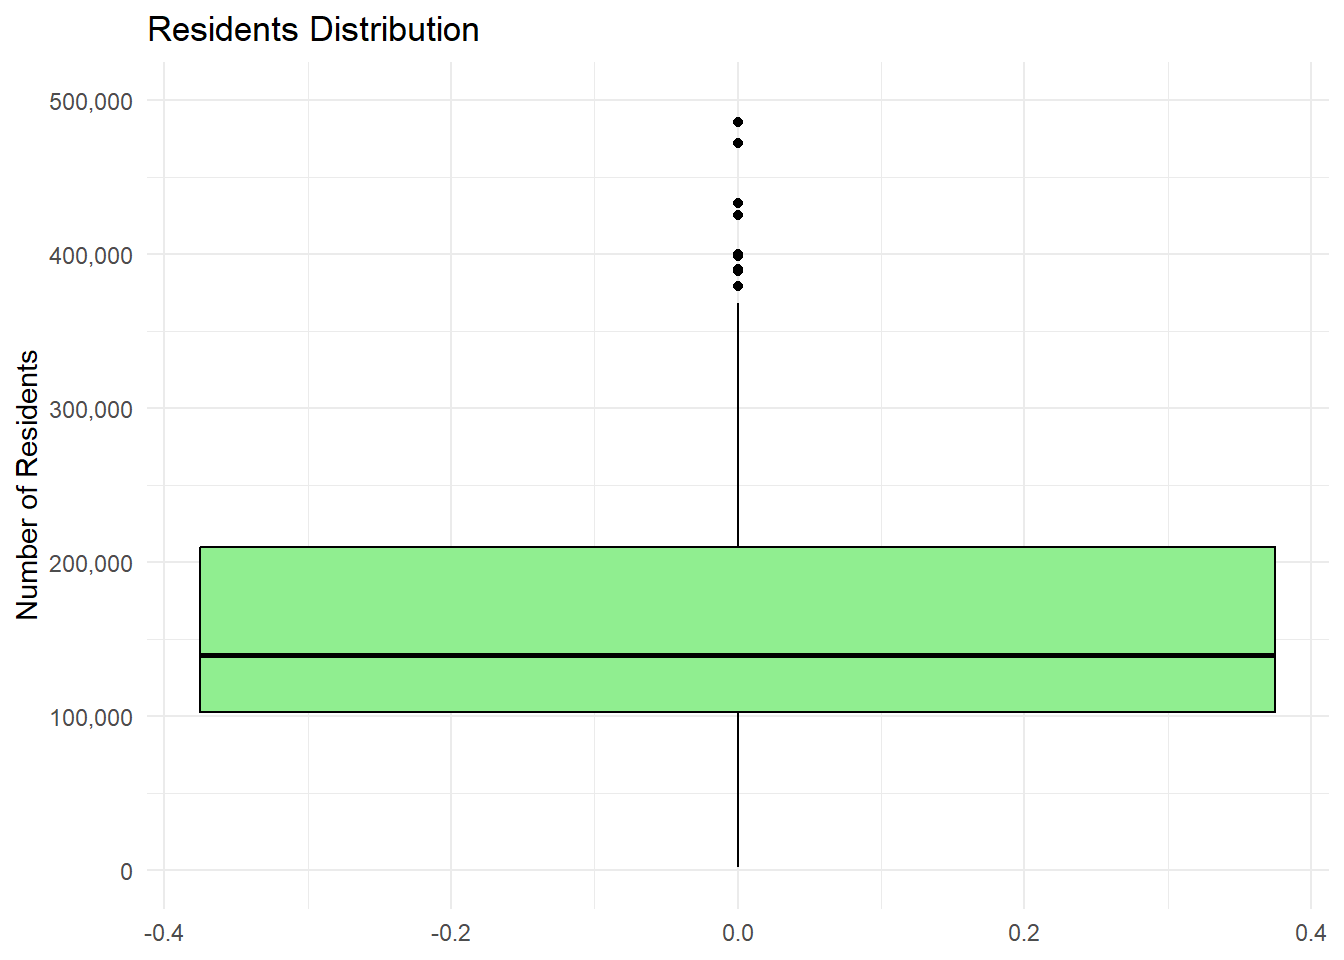
\includegraphics[keepaspectratio]{labs/01.DataExploration_files/figure-pdf/unnamed-chunk-18-1.pdf}}

You should see the histogram below. It reveals that the income
distribution is very skewed with few people earning high salaries and
the majority earning just over or less 35,000 annually.

\textbf{Task}: Adopt a regrouping strategy.

You can also cross-tabulate gross (or net) income with any of the other
variables in the FRS to your heart's content -- or can you?

Again, here is important to recall that the income variables in the FRS
are all `scale' variables; in other words, they are precise measures
rather than broad categories. Consequently, every single person in the
FRS potentially has their own unique income value. That could make for a
table c.~44,000 rows long (one row per person) if each person has their
own unique value. The solution is to create a categorical version of the
original income variable by assigning each person to one of a set of
income categories (income bands). Having done this, cross-tabulation
then becomes possible.

But which strategy to use? Equal intervals, percentiles or `ad hoc'.
Here I would suggest that `ad hoc' is best: all you want to do is to
allocate each independent adult to one of three arbitrarily defined
groups: `low', `middle' and `high' income. \textbf{Define \texttt{Low}
and \texttt{High} Income Thresholds}

Define thresholds for income categories:

\begin{itemize}
\tightlist
\item
  Low-income threshold: £\_\_\_\_\_\_\_\_
\item
  High-income threshold: £\_\_\_\_\_\_\_
\end{itemize}

\textbf{Task}: Create a New Variable Based on Regrouping of Original
Variable.

Recode \texttt{income\_gross} into categories based on the chosen
thresholds.

\begin{Shaded}
\begin{Highlighting}[]
\CommentTok{\# Define thresholds for income categories }
\NormalTok{LOW\_THRESHOLD }\OtherTok{\textless{}{-}} \DecValTok{10000} \CommentTok{\# Replace with the upper limit for low income }
\NormalTok{HIGH\_THRESHOLD }\OtherTok{\textless{}{-}} \DecValTok{50000} \CommentTok{\# Replace with the lower limit for high income }

\CommentTok{\# Define income categories based on thresholds }
\NormalTok{frs\_independent }\OtherTok{\textless{}{-}}\NormalTok{ frs\_independent }\SpecialCharTok{\%\textgreater{}\%} 
    \FunctionTok{mutate}\NormalTok{(}\AttributeTok{income\_category =} \FunctionTok{case\_when}\NormalTok{( }
\NormalTok{        income\_gross }\SpecialCharTok{\textless{}=}\NormalTok{ LOW\_THRESHOLD }\SpecialCharTok{\textasciitilde{}} \StringTok{"Low"}\NormalTok{, }
\NormalTok{        income\_gross }\SpecialCharTok{\textgreater{}=}\NormalTok{ HIGH\_THRESHOLD }\SpecialCharTok{\textasciitilde{}} \StringTok{"High"}\NormalTok{, }
        \ConstantTok{TRUE} \SpecialCharTok{\textasciitilde{}} \StringTok{"Middle"}\NormalTok{ ))}
\end{Highlighting}
\end{Shaded}

The \texttt{mutate()} function in R, from the \textbf{dplyr} package, is
used to add or modify columns in a data frame. It allows you to create
new variables or transform existing ones by applying calculations or
conditional statements directly within the function.

Explanation of the code

\begin{itemize}
\tightlist
\item
  \textbf{\texttt{frs\_independent\ \%\textgreater{}\%}}: The pipe
  operator \texttt{\%\textgreater{}\%} sends \texttt{frs\_independent}
  into \texttt{mutate()}, allowing us to apply transformations without
  reassigning it repeatedly.
\item
  \textbf{\texttt{mutate()}}: Starts the transformation process by
  defining new or modified columns.
\item
  \textbf{\texttt{income\_category\ =\ case\_when(...)}}:

  \begin{itemize}
  \tightlist
  \item
    This creates a new column named \texttt{income\_category}.
  \item
    The \texttt{case\_when()} function defines conditions for assigning
    values to this new column.
  \end{itemize}
\item
  \textbf{\texttt{case\_when()}}:

  \begin{itemize}
  \tightlist
  \item
    \texttt{case\_when()} is used here to assign categorical labels
    based on conditions.
  \item
    \texttt{income\_gross\ \textless{}=\ LOW\_THRESHOLD\ \textasciitilde{}\ "Low"}:
    If \texttt{income\_gross} is less than or equal to
    \texttt{LOW\_THRESHOLD}, \texttt{income\_category} will be labeled
    ``Low.''
  \item
    \texttt{income\_gross\ \textgreater{}=\ HIGH\_THRESHOLD\ \textasciitilde{}\ "High"}:
    If \texttt{income\_gross} is greater than or equal to
    \texttt{HIGH\_THRESHOLD}, \texttt{income\_category} will be labeled
    ``High.''
  \item
    \texttt{TRUE\ \textasciitilde{}\ "Middle"}: Any values not meeting
    the previous conditions are labeled ``Middle.''
  \end{itemize}
\end{itemize}

\textbf{Task}: Add some Metadata.

Define metadata for the new variable by labeling income categories.

\begin{Shaded}
\begin{Highlighting}[]
\CommentTok{\# Add metadata by converting to a factor and defining labels}

\NormalTok{frs\_independent}\SpecialCharTok{$}\NormalTok{income\_category }\OtherTok{\textless{}{-}} \FunctionTok{factor}\NormalTok{(frs\_independent}\SpecialCharTok{$}\NormalTok{income\_category,}
                        \AttributeTok{levels =} \FunctionTok{c}\NormalTok{(}\StringTok{"Low"}\NormalTok{, }\StringTok{"Middle"}\NormalTok{, }\StringTok{"High"}\NormalTok{), }\AttributeTok{labels =} \FunctionTok{c}\NormalTok{(}\StringTok{"\textless{}= £10,000"}\NormalTok{, }\StringTok{"£10,001 {-} £49,999"}\NormalTok{, }\StringTok{"\textgreater{}= £50,000"}\NormalTok{))}
\end{Highlighting}
\end{Shaded}

\textbf{Task}: Check your work.

Examine the frequency distribution of the variable you have just
created. Both variables should have the same number of missing cases,
unless:

\begin{itemize}
\tightlist
\item
  Missing cases in the old variable have been intentionally converted
  into valid cases in the new variable.
\item
  You forgot to allocate a new value to one of the old variable
  categories, in which case the new variable will have more missing
  cases than the old variable.
\end{itemize}

\begin{Shaded}
\begin{Highlighting}[]
\CommentTok{\# Frequency distribution of income categories}
\FunctionTok{table}\NormalTok{(frs\_independent}\SpecialCharTok{$}\NormalTok{income\_category)}
\end{Highlighting}
\end{Shaded}

\begin{verbatim}

       <= £10,000 £10,001 - £49,999        >= £50,000 
             8584             22981              2271 
\end{verbatim}

After preparing the data, use cross-tabulations to compare income levels
across demographic groups.

\begin{Shaded}
\begin{Highlighting}[]
\CommentTok{\# Cross{-}tabulate income category by age group, nationality, etc.}
\FunctionTok{table}\NormalTok{(frs\_independent}\SpecialCharTok{$}\NormalTok{income\_category, frs\_independent}\SpecialCharTok{$}\NormalTok{age\_group)}
\end{Highlighting}
\end{Shaded}

\begin{verbatim}
                   
                    16-19 20-24 25-29 30-34 35-39 40-44 45-49 50-54 55-59 60-64
  <= £10,000          373   680   492   558   474   511   554   652   781   826
  £10,001 - £49,999   263  1241  1802  2056  2052  1948  1995  1967  1749  1772
  >= £50,000            1     8    59   186   314   331   334   356   237   177
                   
                    65-69 70-74  75+
  <= £10,000          773   744 1166
  £10,001 - £49,999  2073  1554 2509
  >= £50,000          144    56   68
\end{verbatim}

Explore income distribution across different regions.

\begin{Shaded}
\begin{Highlighting}[]
\CommentTok{\# Cross{-}tabulate income category by region}
\FunctionTok{table}\NormalTok{(frs\_independent}\SpecialCharTok{$}\NormalTok{income\_category, frs\_independent}\SpecialCharTok{$}\NormalTok{region) }
\end{Highlighting}
\end{Shaded}

\begin{verbatim}
                   
                    East Midlands East of England London North East North West
  <= £10,000                  562             665    740        357        878
  £10,001 - £49,999          1550            1855   1850        979       2347
  >= £50,000                  135             245    367         48        174
                   
                    Northern Ireland Scotland South East South West Wales
  <= £10,000                     874     1212        895        588   399
  £10,001 - £49,999             2305     3234       2563       1707   971
  >= £50,000                     123      322        367        149    63
                   
                    West Midlands Yorks and the Humber
  <= £10,000                  744                  670
  £10,001 - £49,999          1892                 1728
  >= £50,000                  164                  114
\end{verbatim}

\textbf{Tips for Cross-Tabulation}

\begin{itemize}
\tightlist
\item
  Place the income variable in the columns.
\item
  Add multiple variables in the rows to create simultaneous
  cross-tabulations.
\end{itemize}

\bookmarksetup{startatroot}

\chapter{Lab: Correlation, Single, and Multiple Linear
Regression}\label{lab-correlation-single-and-multiple-linear-regression}

\textbf{IMPORTANT: Before starting: verify that you have set the
directory correctly and familiarise yourself with working with
directories and loading files. These are the
\href{https://gdsl-ul.github.io/stats/general/wdPaths.html}{instructions}}.

\textbf{Now create a .qmd project. We use the
\texttt{File\ -\textgreater{}\ New\ File\ -\textgreater{}\ Quarto\ Document..}
dropdown option; a menu will appear asking you for the document title,
author, and preferred output type. You can select HTML. Call it
``\emph{week2}'' and save it in your main folder.}

Follow the practical below. You can describe what you are doing in
normal text. See
\href{https://quarto.org/docs/authoring/markdown-basics.html}{here} for
how to format normal text in Markdown documents

In this week's practical, we will review how to calculate and visualise
correlation coefficients between variables. This practical is split into
two parts. The first part focuses on measuring and visualising the
relationship between between \textbf{continuous variables}. The second
part goes through the implementation of a Linear Regression Model, again
between continuous variables.

Before getting into it, have a look at this
\href{https://mlu-explain.github.io/linear-regression/}{resource}, it
really helps understand how regression models work.

The lecture's slides can be found
\href{https://github.com/GDSL-UL/stats/blob/main/lectures/lecture08.pdf}{here}.

Before completing the practical, please take this
\href{https://canvas.liverpool.ac.uk/courses/84668/quizzes/169285?module_item_id=2435564}{quiz}.

\textbf{Learning Objectives:}

\begin{itemize}
\tightlist
\item
  Visualise the association between two continuous variables using a
  scatterplot.
\item
  Measure the strength of the association between two variables by
  calculating their correlation coefficient.
\item
  Build a formal regression model.
\item
  Understand how to estimate and interpret a multiple linear regression
  model.
\end{itemize}

\emph{Note on file paths}: When calling the \texttt{read.csv} function,
the path will vary depending on the location of the script it is being
executed or your working directory (WD):

\begin{enumerate}
\def\labelenumi{\arabic{enumi}.}
\tightlist
\item
  \textbf{If the script or your WD is in a sub-folder} (e.g.,
  \texttt{labs}), use
  \texttt{"../data/Census2021/EW\_DistrictPercentages.csv"}. The
  \texttt{..} tells R to go one level up to the main directory
  (\texttt{stats/}) and then access the \texttt{data/} folder.
  \textbf{Example}:
  \texttt{read.csv("../data/Census2021/EW\_DistrictPercentages.csv")}.
\item
  \textbf{If the script is in the main directory} (e.g.~inside
  \texttt{stats/}), you can access the data directly using
  \texttt{"data/Census2021/EW\_DistrictPercentages.csv"}. Here, no
  \texttt{..} is necessary as the \texttt{data/} folder is directly
  accessible from the working directory. \textbf{Example}:
  \texttt{read.csv("data/Census2021/EW\_DistrictPercentages.csv")}
\end{enumerate}

\section{Part I. Correlation}\label{part-i.-correlation}

\subsection{Data Overview: Descriptive
Statistics:}\label{data-overview-descriptive-statistics}

Let's start by picking \textbf{one dataset derived from the
English-Wales 2021 Census data}. You can choose one dataset that
aggregates data either at a) county, b) district, or c) ward-level.
Lower Tier Local Authority-, Region-, and Country-level data is also
available in the data folder.

see also:
https://canvas.liverpool.ac.uk/courses/77895/pages/census-data-2021

\begin{Shaded}
\begin{Highlighting}[]
\CommentTok{\# Load necessary libraries }
\FunctionTok{library}\NormalTok{(ggplot2) }
\end{Highlighting}
\end{Shaded}

\begin{verbatim}
Warning: package 'ggplot2' was built under R version 4.5.1
\end{verbatim}

\begin{Shaded}
\begin{Highlighting}[]
\FunctionTok{library}\NormalTok{(dplyr) }
\end{Highlighting}
\end{Shaded}

\begin{verbatim}
Warning: package 'dplyr' was built under R version 4.5.1
\end{verbatim}

\begin{verbatim}

Attaching package: 'dplyr'
\end{verbatim}

\begin{verbatim}
The following objects are masked from 'package:stats':

    filter, lag
\end{verbatim}

\begin{verbatim}
The following objects are masked from 'package:base':

    intersect, setdiff, setequal, union
\end{verbatim}

\begin{Shaded}
\begin{Highlighting}[]
\FunctionTok{options}\NormalTok{(}\AttributeTok{scipen =} \DecValTok{999}\NormalTok{, }\AttributeTok{digits =} \DecValTok{4}\NormalTok{)  }\CommentTok{\# Avoid scientific notation and round to 4 decimals globally}

\CommentTok{\# load data {-} you main need to remove "../"}
\NormalTok{census }\OtherTok{\textless{}{-}} \FunctionTok{read.csv}\NormalTok{(}\StringTok{"../data/Census2021/EW\_DistrictPercentages.csv"}\NormalTok{) }\CommentTok{\# District level}
\end{Highlighting}
\end{Shaded}

We're using a (district/ward/etc.) level census dataset that includes:

\begin{itemize}
\tightlist
\item
  \% of population with poor health (variable name:
  \texttt{pct\_Very\_bad\_health}).
\item
  \% of population with no qualifications
  (\texttt{pct\_No\_qualifications}).
\item
  \% of male population (\texttt{pct\_Males}).
\item
  \% of population in a higher managerial/professional occupation
  (\texttt{pct\_Higher\_manager\_prof}).
\end{itemize}

First, let's get some descriptive statistics that help identify general
trends and distributions in the data.

\begin{Shaded}
\begin{Highlighting}[]
\CommentTok{\# Summary statistics}
\NormalTok{summary\_data }\OtherTok{\textless{}{-}}\NormalTok{ census }\SpecialCharTok{\%\textgreater{}\%}
  \FunctionTok{select}\NormalTok{(pct\_Very\_bad\_health, pct\_No\_qualifications, pct\_Males, pct\_Higher\_manager\_prof) }\SpecialCharTok{\%\textgreater{}\%}
  \FunctionTok{summarise\_all}\NormalTok{(}\FunctionTok{list}\NormalTok{(}\AttributeTok{mean =}\NormalTok{ mean, }\AttributeTok{sd =}\NormalTok{ sd))}
\NormalTok{summary\_data}
\end{Highlighting}
\end{Shaded}

\begin{verbatim}
  pct_Very_bad_health_mean pct_No_qualifications_mean pct_Males_mean
1                    1.173                       17.9          48.97
  pct_Higher_manager_prof_mean pct_Very_bad_health_sd pct_No_qualifications_sd
1                        13.22                 0.3401                    3.959
  pct_Males_sd pct_Higher_manager_prof_sd
1       0.6605                       4.73
\end{verbatim}

\textbf{Q1}. Complete the table below by specifying each variable type
(continuous or categorical) and reporting its mean and standard
deviation.

\begin{longtable}[]{@{}
  >{\raggedright\arraybackslash}p{(\linewidth - 6\tabcolsep) * \real{0.2500}}
  >{\raggedright\arraybackslash}p{(\linewidth - 6\tabcolsep) * \real{0.2500}}
  >{\raggedright\arraybackslash}p{(\linewidth - 6\tabcolsep) * \real{0.2500}}
  >{\raggedright\arraybackslash}p{(\linewidth - 6\tabcolsep) * \real{0.2500}}@{}}
\toprule\noalign{}
\begin{minipage}[b]{\linewidth}\raggedright
Variable Name
\end{minipage} & \begin{minipage}[b]{\linewidth}\raggedright
Type (Continuous or Categorical)
\end{minipage} & \begin{minipage}[b]{\linewidth}\raggedright
Mean
\end{minipage} & \begin{minipage}[b]{\linewidth}\raggedright
Standard Deviation
\end{minipage} \\
\midrule\noalign{}
\endhead
\bottomrule\noalign{}
\endlastfoot
pct\_Very\_bad\_health & & & \\
pct\_No\_qualifications & & & \\
pct\_Males & & & \\
pct\_Higher\_manager\_prof & & & \\
\end{longtable}

\subsection{Simple visualisation for continuous
data}\label{simple-visualisation-for-continuous-data}

You can visualise the relationship between two continuous variables
using a scatter plot. Using the chosen census datasets, visualise the
association between the \% of population with bad health
(\texttt{pct\_Very\_bad\_health}) and each of the following:

\begin{itemize}
\tightlist
\item
  the \% of population with no qualifications
  (\texttt{pct\_No\_qualifications});
\item
  the \% of population aged 65 to 84 (\texttt{pct\_Age\_65\_to\_84});
\item
  the \% of population in a married couple
  (\texttt{pct\_Married\_opposite\_sex\_couple});
\item
  the \% of population in a Higher Managerial or Professional occupation
  (\texttt{pct\_Higher\_manager\_prof}).
\end{itemize}

\begin{Shaded}
\begin{Highlighting}[]
\CommentTok{\# 1}
\FunctionTok{ggplot}\NormalTok{(census, }\FunctionTok{aes}\NormalTok{(}\AttributeTok{x =}\NormalTok{ pct\_No\_qualifications, }\AttributeTok{y =}\NormalTok{ pct\_Very\_bad\_health)) }\SpecialCharTok{+}
    \FunctionTok{geom\_point}\NormalTok{() }\SpecialCharTok{+} 
    \FunctionTok{labs}\NormalTok{(}\AttributeTok{title =} \FunctionTok{paste}\NormalTok{(}\StringTok{"Scatterplot of \% people in Very bad health vs \& \% people"}\NormalTok{, }\StringTok{"No Qualifications"}\NormalTok{), }
         \AttributeTok{x =} \StringTok{"\% no qualifications"}\NormalTok{, }\AttributeTok{y =} \StringTok{"\% Very bad\_health"}\NormalTok{) }\SpecialCharTok{+}
    \FunctionTok{theme\_minimal}\NormalTok{()}
\end{Highlighting}
\end{Shaded}

\pandocbounded{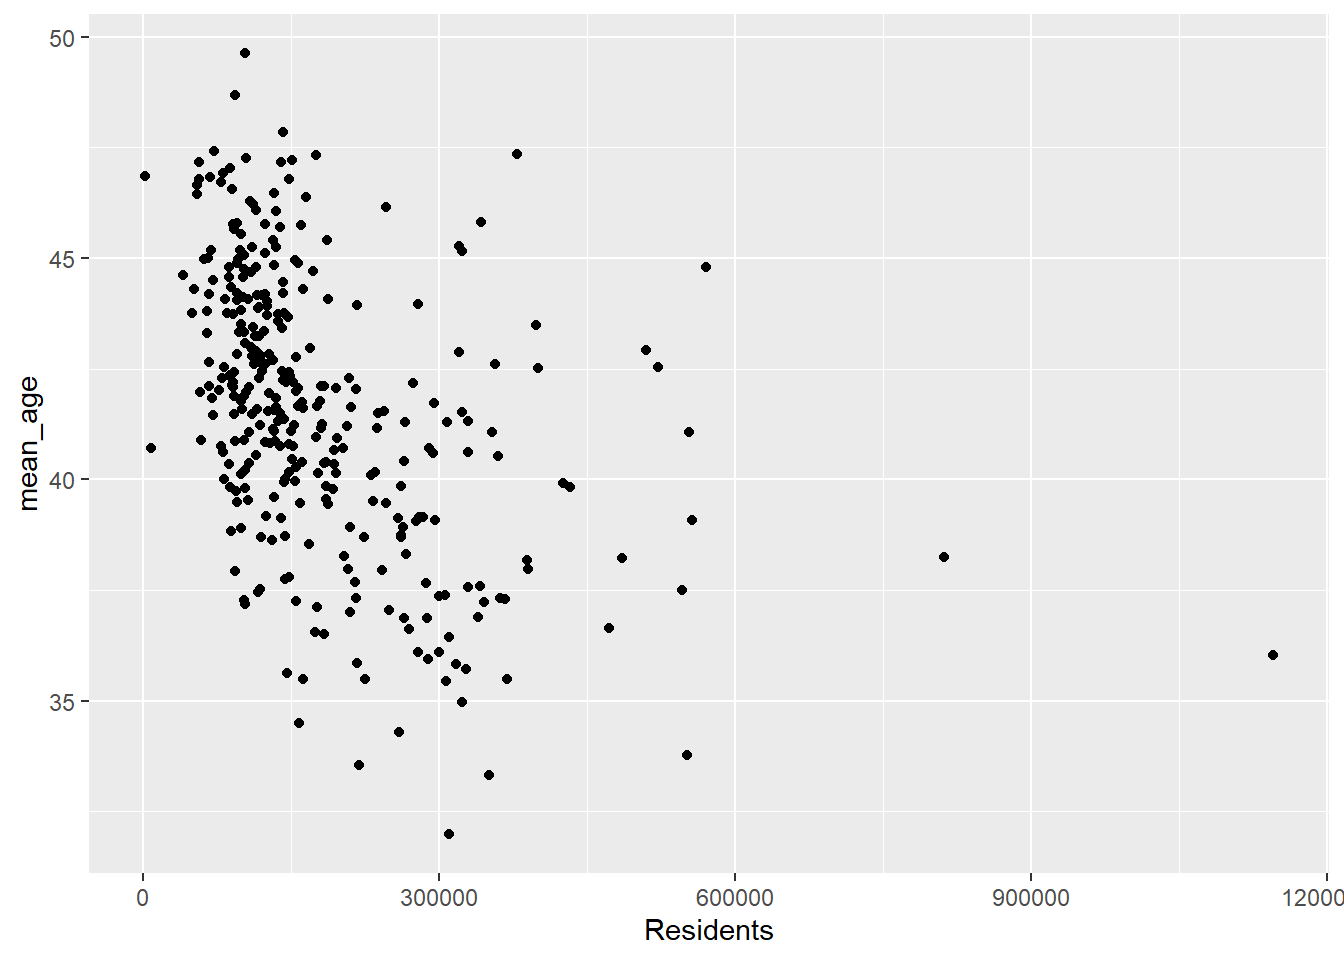
\includegraphics[keepaspectratio]{labs/02.MultipleLinear_files/figure-pdf/unnamed-chunk-3-1.pdf}}

\begin{Shaded}
\begin{Highlighting}[]
\CommentTok{\# 2}
\FunctionTok{ggplot}\NormalTok{(census, }\FunctionTok{aes}\NormalTok{(}\AttributeTok{x =}\NormalTok{ pct\_Age\_65\_to\_84, }\AttributeTok{y =}\NormalTok{ pct\_Very\_bad\_health)) }\SpecialCharTok{+}
    \FunctionTok{geom\_point}\NormalTok{() }\SpecialCharTok{+} 
    \FunctionTok{labs}\NormalTok{(}\AttributeTok{title =} \FunctionTok{paste}\NormalTok{(}\StringTok{"Scatterplot of \% people in Very bad health vs \& \% people"}\NormalTok{, }\StringTok{"aged between 65 and 84"}\NormalTok{),}
         \AttributeTok{x =} \StringTok{"\% aged 65{-}84"}\NormalTok{, }\AttributeTok{y =} \StringTok{"\% Very bad\_health"}\NormalTok{) }\SpecialCharTok{+}
    \FunctionTok{theme\_minimal}\NormalTok{()}
\end{Highlighting}
\end{Shaded}

\pandocbounded{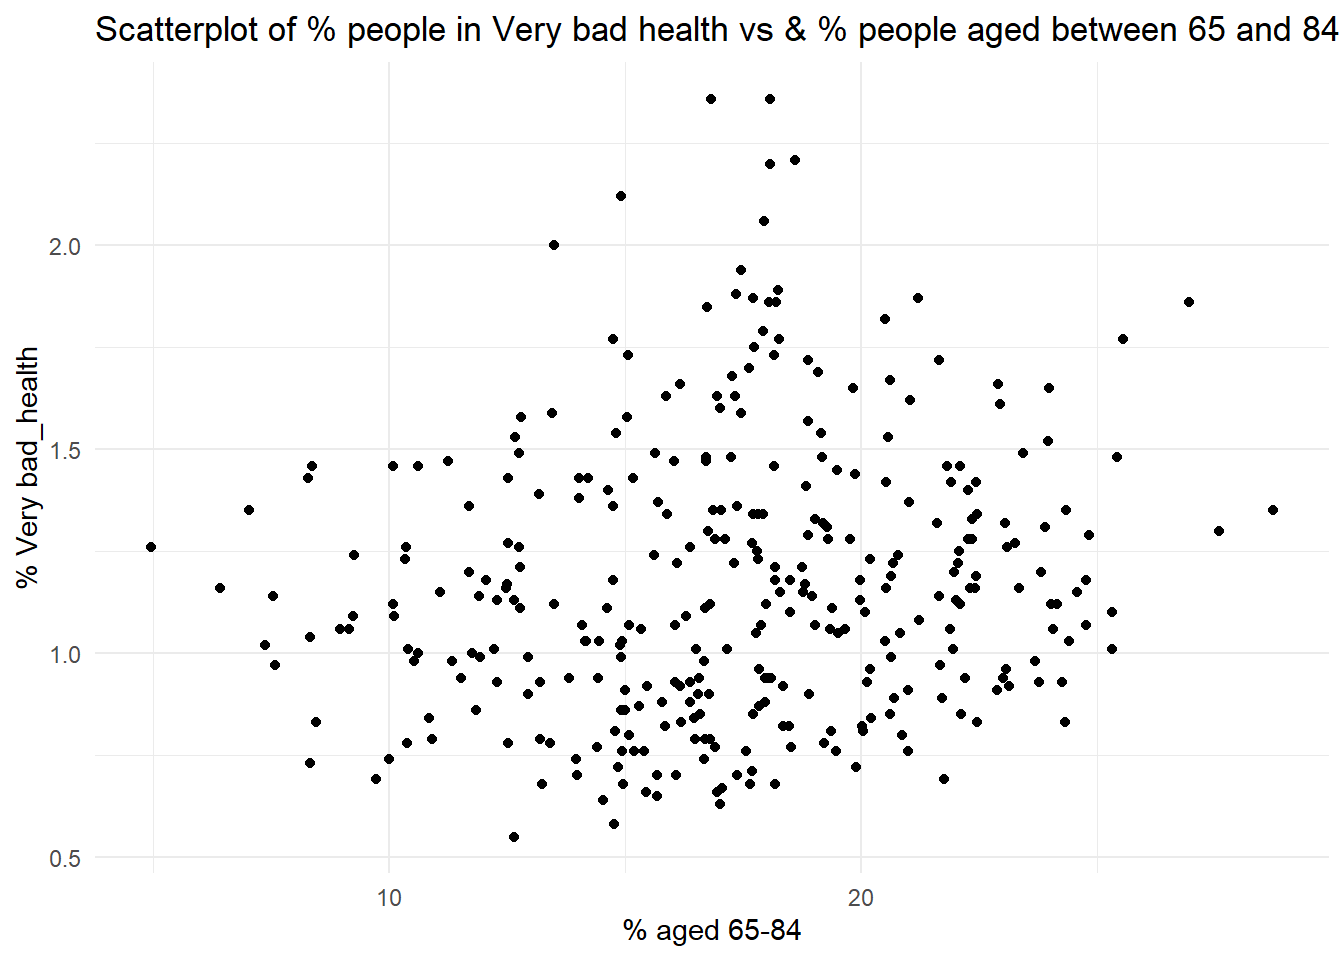
\includegraphics[keepaspectratio]{labs/02.MultipleLinear_files/figure-pdf/unnamed-chunk-3-2.pdf}}

\begin{Shaded}
\begin{Highlighting}[]
\CommentTok{\# 3}
\FunctionTok{ggplot}\NormalTok{(census, }\FunctionTok{aes}\NormalTok{(}\AttributeTok{x =}\NormalTok{ pct\_Married\_opposite\_sex\_couple, }\AttributeTok{y =}\NormalTok{ pct\_Very\_bad\_health)) }\SpecialCharTok{+}
    \FunctionTok{geom\_point}\NormalTok{() }\SpecialCharTok{+} 
    \FunctionTok{labs}\NormalTok{(}\AttributeTok{title =} \FunctionTok{paste}\NormalTok{(}\StringTok{"Scatterplot of \% people in Very bad health vs \& \% people"}\NormalTok{, }\StringTok{"in married couples."}\NormalTok{), }
         \AttributeTok{x =} \StringTok{"\% married couples"}\NormalTok{, }\AttributeTok{y =} \StringTok{"\% Very bad\_health"}\NormalTok{) }\SpecialCharTok{+}
    \FunctionTok{theme\_minimal}\NormalTok{()}
\end{Highlighting}
\end{Shaded}

\pandocbounded{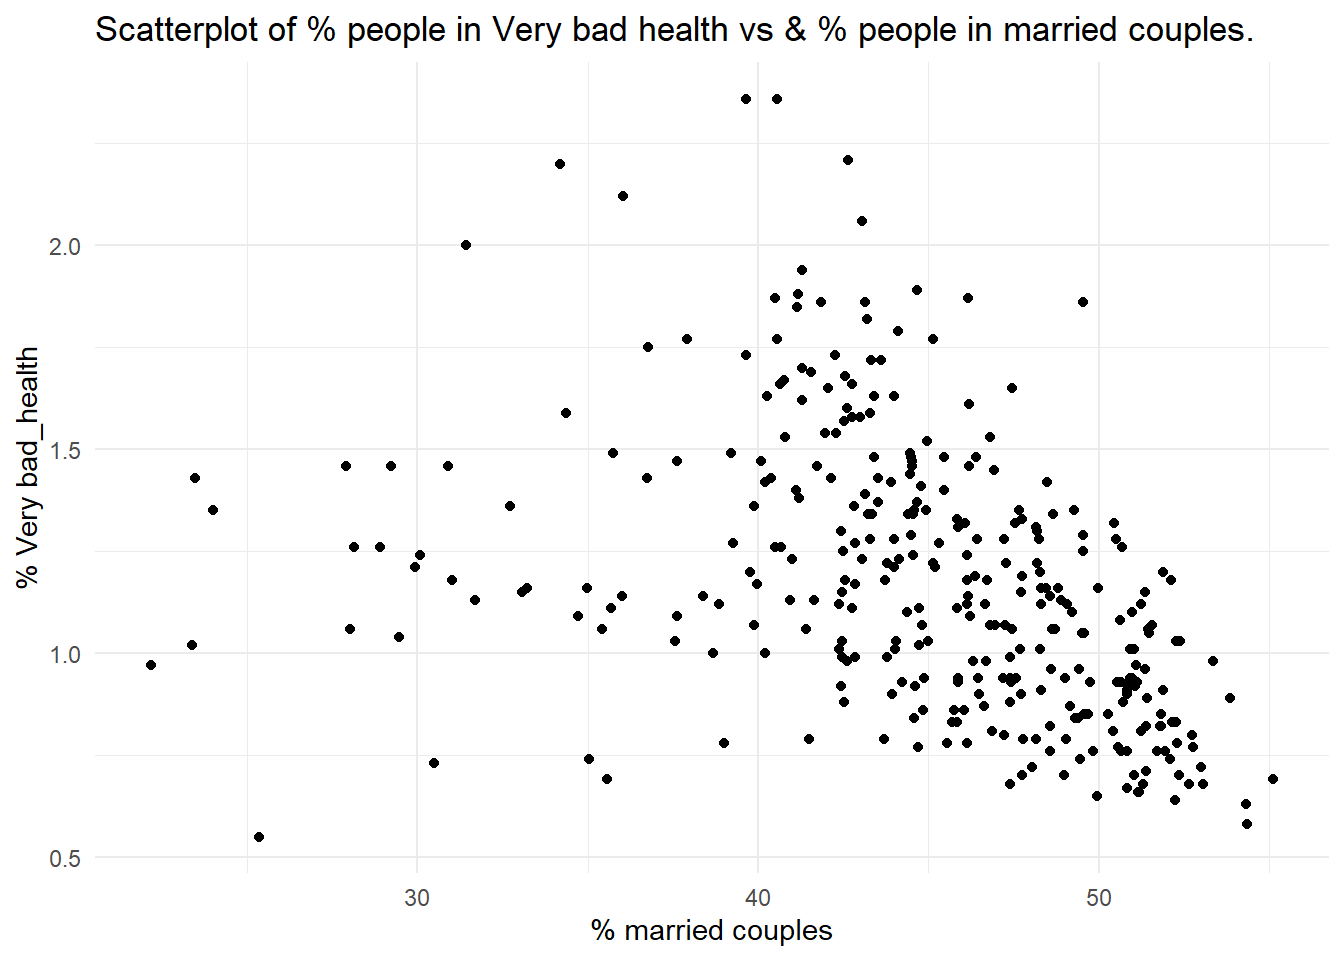
\includegraphics[keepaspectratio]{labs/02.MultipleLinear_files/figure-pdf/unnamed-chunk-3-3.pdf}}

\begin{Shaded}
\begin{Highlighting}[]
\CommentTok{\# 4}
\FunctionTok{ggplot}\NormalTok{(census, }\FunctionTok{aes}\NormalTok{(}\AttributeTok{x =}\NormalTok{ pct\_Higher\_manager\_prof, }\AttributeTok{y =}\NormalTok{ pct\_Very\_bad\_health)) }\SpecialCharTok{+}
    \FunctionTok{geom\_point}\NormalTok{() }\SpecialCharTok{+} 
    \FunctionTok{labs}\NormalTok{(}\AttributeTok{title =} \FunctionTok{paste}\NormalTok{(}\StringTok{"Scatterplot of \% people in Very bad health vs \& \% people"}\NormalTok{, }\StringTok{"in higher managerial professions."}\NormalTok{), }
         \AttributeTok{x =} \StringTok{"\% higher managerial professions"}\NormalTok{, }\AttributeTok{y =} \StringTok{"\% Very bad\_health"}\NormalTok{) }\SpecialCharTok{+}
    \FunctionTok{theme\_minimal}\NormalTok{()}
\end{Highlighting}
\end{Shaded}

\pandocbounded{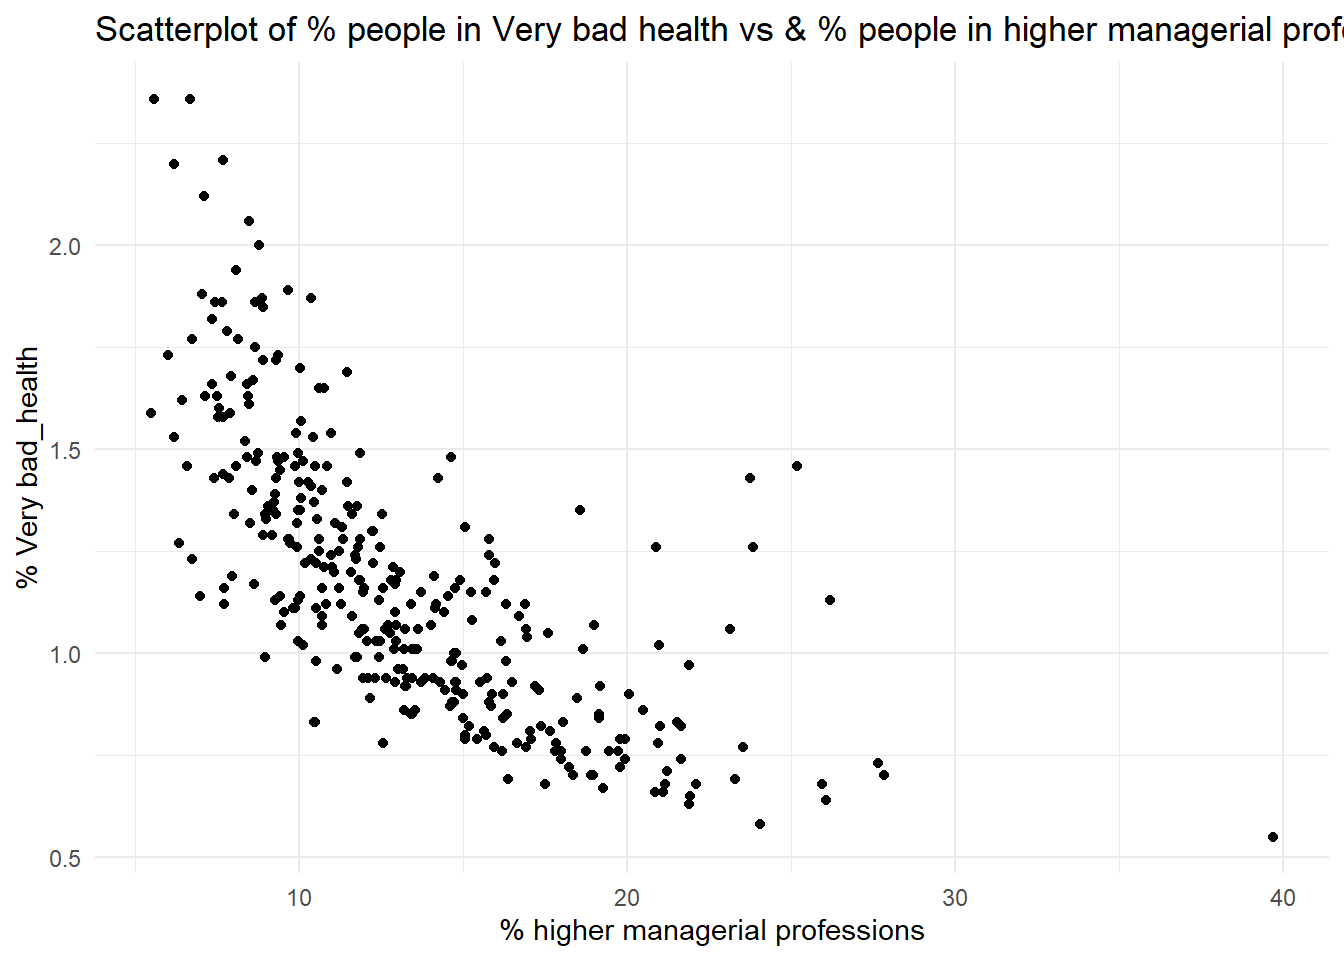
\includegraphics[keepaspectratio]{labs/02.MultipleLinear_files/figure-pdf/unnamed-chunk-3-4.pdf}}

\textbf{Q2. Which of the associations do you think is strongest, which
one is the weakest?}

As noted, before, an observed association between two variables is no
guarantee of causation. It could be that the observed association is:

\begin{itemize}
\tightlist
\item
  simply a chance one due to sampling uncertainty;
\item
  caused by some third underlying variable which explains the spatial
  variation of both of the variables in the scatterplot;
\item
  due to the inherent arbitrariness of the boundaries used to define the
  areas being analysed (the `Modifiable Area Unit Problem').
\end{itemize}

\textbf{Q3. Setting these caveats to one side, are the associations
observed in the scatter-plots suggestive of any causative mechanisms of
bad health?}

Rather than relying upon an impressionistic view of the strength of the
association between two variables, we can measure that association by
calculating the relevant correlation coefficient. The Table below
identifies the statistically appropriate measure of correlation to use
between two continuous variables.

\begin{longtable}[]{@{}
  >{\raggedright\arraybackslash}p{(\linewidth - 4\tabcolsep) * \real{0.5405}}
  >{\raggedright\arraybackslash}p{(\linewidth - 4\tabcolsep) * \real{0.3243}}
  >{\raggedright\arraybackslash}p{(\linewidth - 4\tabcolsep) * \real{0.1351}}@{}}
\toprule\noalign{}
\begin{minipage}[b]{\linewidth}\raggedright
Variable Data Type
\end{minipage} & \begin{minipage}[b]{\linewidth}\raggedright
Measure of Correlation
\end{minipage} & \begin{minipage}[b]{\linewidth}\raggedright
Range
\end{minipage} \\
\midrule\noalign{}
\endhead
\bottomrule\noalign{}
\endlastfoot
Both symmetrically distributed & Pearson's & -1 to +1 \\
One or both with a skewed distribution & Spearman's Rank & -1 to +1 \\
\end{longtable}

\textbf{Different Calculation Methods}: Pearson's correlation assumes
linear relationships and is suitable for symmetrically distributed
(normally distributed) variables, measuring the strength of the linear
relationship. Spearman's rank correlation, however, works on ranked
data, so it's more suitable for skewed data or variables with non-linear
relationships, measuring the strength and direction of a monotonic
relationship.

When calculating correlation for a single pair of variables, select the
method that best fits their data distribution:

\begin{itemize}
\tightlist
\item
  Use \textbf{Pearson's} if both variables are symmetrically
  distributed.
\item
  Use \textbf{Spearman's} if one or both variables are skewed.
\end{itemize}

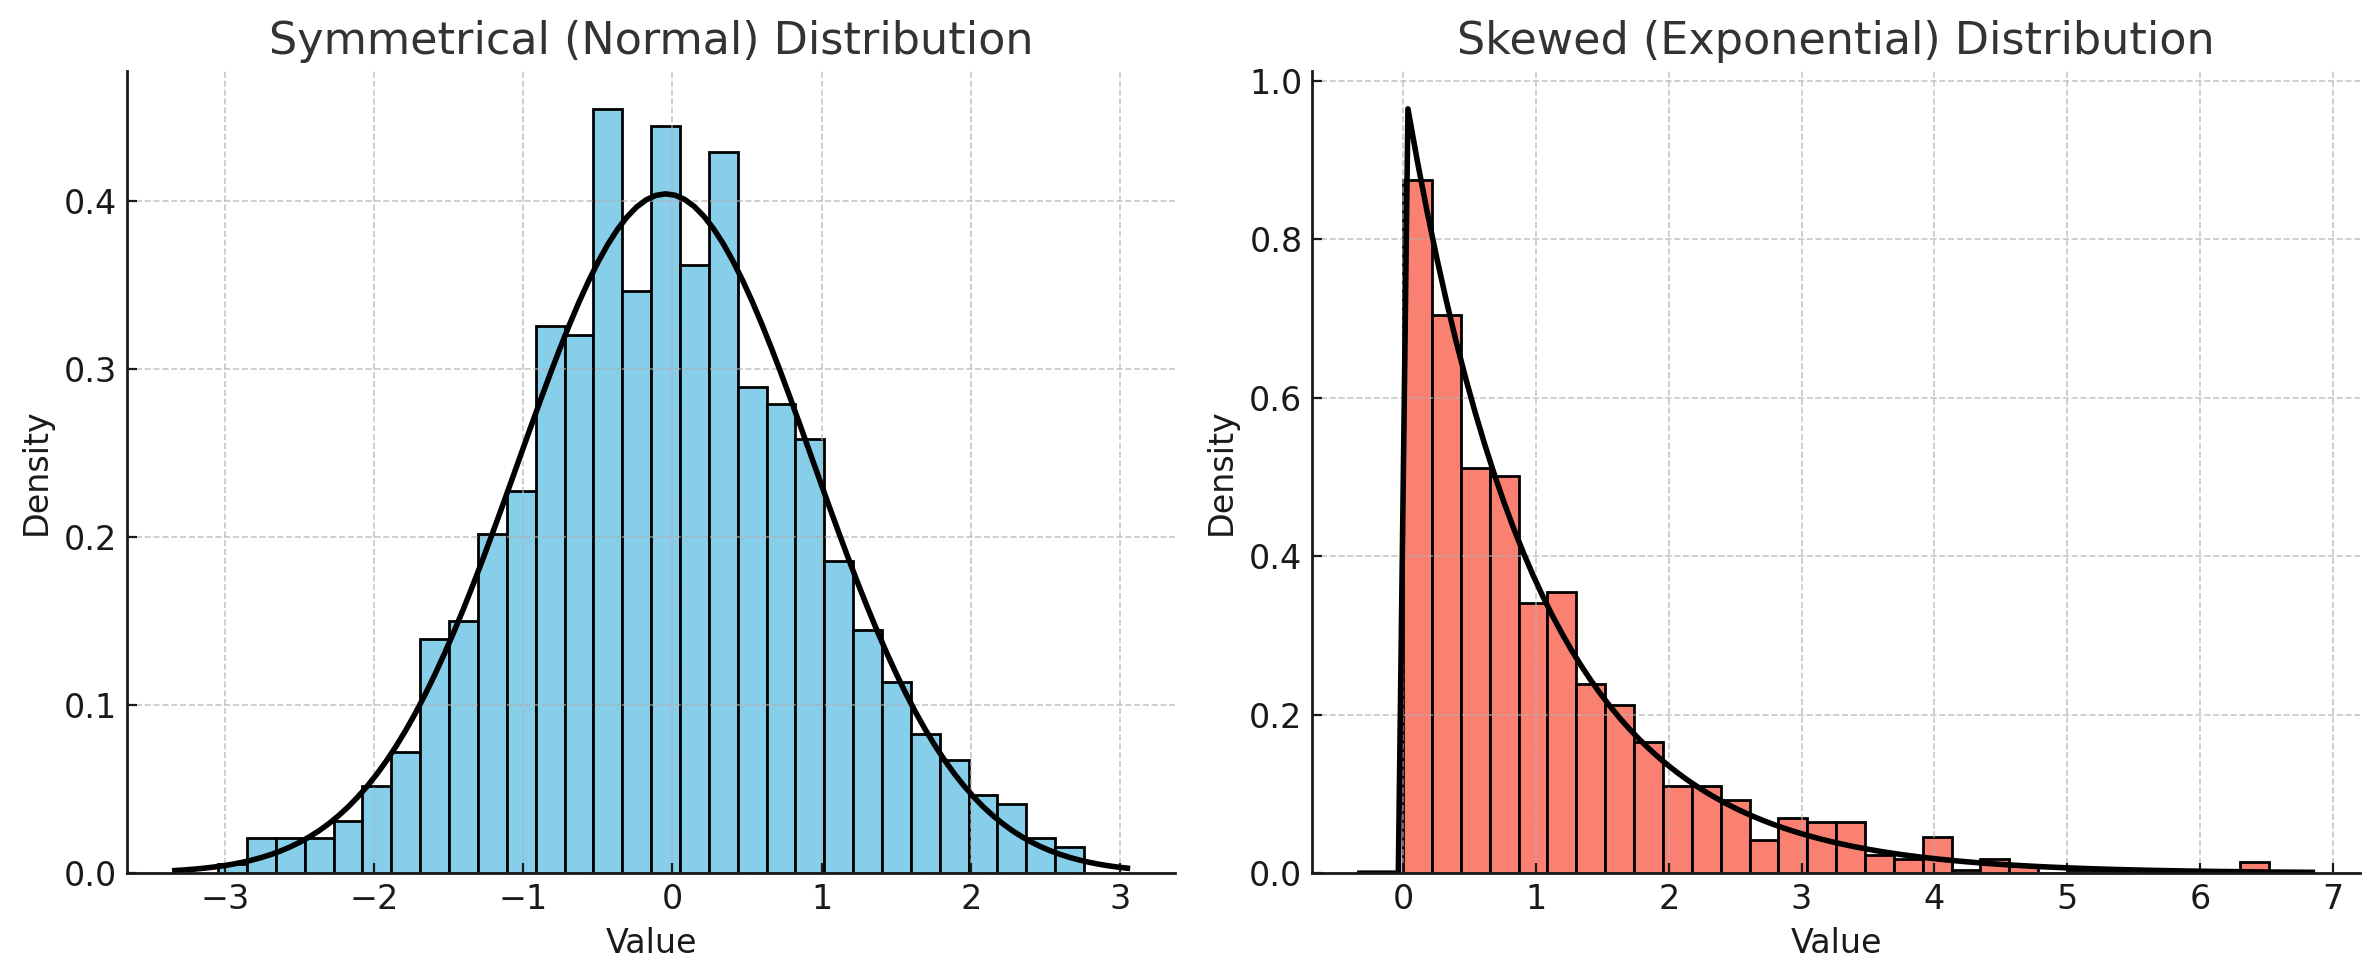
\includegraphics[width=7.93in,height=\textheight,keepaspectratio]{labs/../img/distributions.png}

You can check the distribution of a variable
(e.g.~\texttt{pct\_No\_qualifications} like this):

\begin{Shaded}
\begin{Highlighting}[]
\CommentTok{\# Plot histogram with density overlay for a chosen variable (e.g., \textquotesingle{}pct\_No\_qualifications\textquotesingle{})}
\FunctionTok{ggplot}\NormalTok{(census, }\FunctionTok{aes}\NormalTok{(}\AttributeTok{x =}\NormalTok{ pct\_No\_qualifications)) }\SpecialCharTok{+} 
    \FunctionTok{geom\_histogram}\NormalTok{(}\FunctionTok{aes}\NormalTok{(}\AttributeTok{y =} \FunctionTok{after\_stat}\NormalTok{(density)), }\AttributeTok{bins =} \DecValTok{30}\NormalTok{, }\AttributeTok{color =} \StringTok{"black"}\NormalTok{, }\AttributeTok{fill =} \StringTok{"skyblue"}\NormalTok{, }\AttributeTok{alpha =} \FloatTok{0.7}\NormalTok{) }\SpecialCharTok{+}
    \FunctionTok{geom\_density}\NormalTok{(}\AttributeTok{color =} \StringTok{"darkblue"}\NormalTok{, }\AttributeTok{linewidth =} \DecValTok{1}\NormalTok{) }\SpecialCharTok{+}
    \FunctionTok{labs}\NormalTok{(}\AttributeTok{title =} \StringTok{"Distribution of pct\_No\_qualifications"}\NormalTok{, }\AttributeTok{x =} \StringTok{"Value"}\NormalTok{, }\AttributeTok{y =}  \StringTok{"Density"}\NormalTok{) }\SpecialCharTok{+}
  \FunctionTok{theme\_minimal}\NormalTok{()}
\end{Highlighting}
\end{Shaded}

\pandocbounded{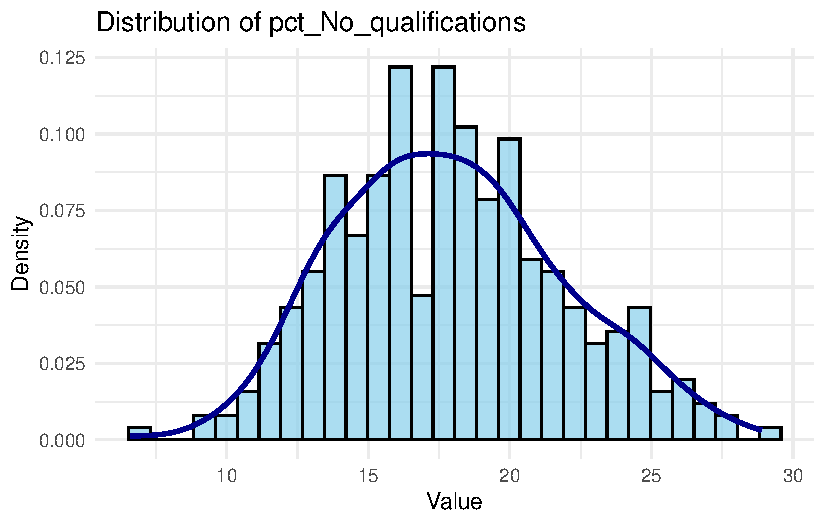
\includegraphics[keepaspectratio]{labs/02.MultipleLinear_files/figure-pdf/unnamed-chunk-5-1.pdf}}

When analyzing multiple pairs of variables, using different measures
(Pearson for some pairs, Spearman for others) creates inconsistencies
since Pearson and Spearman values aren't directly comparable in size due
to their different calculation methods. To maintain consistency across
comparisons, calculate \textbf{both Pearson's and Spearman's
correlations} for each pair, e.g.~do the trends align (both showing
strong, weak, or moderate correlation in the same direction)? This
consistency check can give confidence that the relationships observed
are not dependent on the correlation method chosen. While in a report
you'd typically include only one set of correlations (usually Pearson's
if the relationships appear linear), calculating both can validate that
your observations aren't an artifact of the correlation method.

\textbf{Research Question 1: Which of our selected variables are most
strongly correlated with \% of population with bad health?}

To answer this question, complete the Table below by editing/running
this code:.

Pearson correlations

\begin{Shaded}
\begin{Highlighting}[]
\NormalTok{pearson\_correlation }\OtherTok{\textless{}{-}} \FunctionTok{cor}\NormalTok{(census}\SpecialCharTok{$}\NormalTok{pct\_Very\_bad\_health,}
\NormalTok{    census}\SpecialCharTok{$}\NormalTok{pct\_No\_qualifications,}\AttributeTok{use =} \StringTok{"complete.obs"}\NormalTok{, }\AttributeTok{method =} \StringTok{"pearson"}\NormalTok{)}
    
\CommentTok{\# Display the results}
\FunctionTok{cat}\NormalTok{(}\StringTok{"Pearson Correlation:"}\NormalTok{, pearson\_correlation, }\StringTok{"}\SpecialCharTok{\textbackslash{}n}\StringTok{"}\NormalTok{)}
\end{Highlighting}
\end{Shaded}

\begin{verbatim}
Pearson Correlation: 0.7619 
\end{verbatim}

Spearman correlations:

\begin{Shaded}
\begin{Highlighting}[]
\NormalTok{spearman\_correlation }\OtherTok{\textless{}{-}} \FunctionTok{cor}\NormalTok{(census}\SpecialCharTok{$}\NormalTok{pct\_Very\_bad\_health,}
\NormalTok{    census}\SpecialCharTok{$}\NormalTok{pct\_No\_qualifications, }\AttributeTok{use =} \StringTok{"complete.obs"}\NormalTok{, }\AttributeTok{method =} \StringTok{"spearman"}\NormalTok{)}

\FunctionTok{cat}\NormalTok{(}\StringTok{"Spearman Correlation:"}\NormalTok{, spearman\_correlation, }\StringTok{"}\SpecialCharTok{\textbackslash{}n}\StringTok{"}\NormalTok{)}
\end{Highlighting}
\end{Shaded}

\begin{verbatim}
Spearman Correlation: 0.7781 
\end{verbatim}

\begin{longtable}[]{@{}
  >{\raggedright\arraybackslash}p{(\linewidth - 4\tabcolsep) * \real{0.7432}}
  >{\raggedright\arraybackslash}p{(\linewidth - 4\tabcolsep) * \real{0.1216}}
  >{\raggedright\arraybackslash}p{(\linewidth - 4\tabcolsep) * \real{0.1351}}@{}}
\toprule\noalign{}
\begin{minipage}[b]{\linewidth}\raggedright
Covariates
\end{minipage} & \begin{minipage}[b]{\linewidth}\raggedright
Pearson
\end{minipage} & \begin{minipage}[b]{\linewidth}\raggedright
Spearman
\end{minipage} \\
\midrule\noalign{}
\endhead
\bottomrule\noalign{}
\endlastfoot
pct\_Very\_bad\_health - pct\_No\_qualifications & & \\
pct\_Very\_bad\_health - pct\_Age\_65\_to\_84 & & \\
pct\_Very\_bad\_health - pct\_Married\_opposite\_sex\_couple & & \\
pct\_Very\_bad\_health - pct\_Higher\_manager\_prof & & \\
\end{longtable}

\textbf{What can you make of this numbers?}

If you think you have found a correlation between two variables in our
dataset, this doesn't mean that an association exists between these two
variables in the population at large. The uncertainty arises because, by
chance, the random sample included in our dataset might not be fully
representative of the wider population.

For this reason, we need to verify whether the correlation is
statistically significant,

\begin{Shaded}
\begin{Highlighting}[]
\CommentTok{\# significance test for pearson, for example}
\NormalTok{pearson\_test }\OtherTok{\textless{}{-}} \FunctionTok{cor.test}\NormalTok{(census}\SpecialCharTok{$}\NormalTok{pct\_Very\_bad\_health,}
\NormalTok{    census}\SpecialCharTok{$}\NormalTok{pct\_No\_qualifications, }\AttributeTok{method =} \StringTok{"pearson"}\NormalTok{, }\AttributeTok{use =} \StringTok{"complete.obs"}\NormalTok{)}
\NormalTok{pearson\_test}
\end{Highlighting}
\end{Shaded}

\begin{verbatim}

    Pearson's product-moment correlation

data:  census$pct_Very_bad_health and census$pct_No_qualifications
t = 21, df = 329, p-value <0.0000000000000002
alternative hypothesis: true correlation is not equal to 0
95 percent confidence interval:
 0.7127 0.8037
sample estimates:
   cor 
0.7619 
\end{verbatim}

Look at
https://www.rdocumentation.org/packages/stats/versions/3.6.2/topics/cor.test
for details about the function. But in general, when calculating the
correlation between two variables, a \textbf{p-value} accompanies the
correlation coefficient to indicate the statistical significance of the
observed association. This p-value tests the null hypothesis that there
is no association between the two variables (i.e., that the correlation
is zero).

When interpreting p-values, certain thresholds denote different levels
of confidence. A p-value less than 0.05 is generally considered
statistically significant at the 95\% confidence level, suggesting that
we can be 95\% confident there is an association between the variables
in the broader population. When the p-value is below 0.01, the result is
significant at the 99\% confidence level, meaning we have even greater
confidence (99\%) that an association exists. Sometimes, on research
papers or tables significance levels are denoted with asterisks: one
asterisk (\texttt{*}) typically indicates significance at the 95\% level
(p \textless{} 0.05), two asterisks (\texttt{**}) significance at the
99\% level (p \textless{} 0.01), three asterisks (\texttt{***})
significance at the 99.99\% level (p \textless{} 0.01).

Typically, p-values are reported under labels such as ``Sig
(2-tailed),'' where ``2-tailed'' refers to the fact that the test
considers both directions (positive and negative correlations).
Reporting the exact p-value (e.g., p = 0.002) is more informative than
using thresholds alone, as it gives a clearer picture of how strongly
the data contradicts the null hypothesis of no association.

\textbf{In a nutshell, lower p-values suggest a stronger statistical
basis for believing that an observed correlation is not due to random
chance. A statistically significant p-value reinforces confidence that
an association is likely to exist in the wider population, though it
does not imply causation.}

\subsection{Part. 2: Implementing a Linear Regression
Model}\label{part.-2-implementing-a-linear-regression-model}

A key goal of data analysis is to explore the potential factors of
health at the local district level. So far, we have used
cross-tabulations and various bivariate correlation analysis methods to
explore the relationships between variables. One key limitation of
standard correlation analysis is that it remains hard to look at the
associations of an outcome/dependent variable to multiple
independent/explanatory variables at the same time. Regression analysis
provides a very useful and flexible methodological framework for such a
purpose. Therefore, we will investigate how various local factors impact
residents' health by building a multiple linear regression model in R.

We use \texttt{pct\_Very\_bad\_health} as a proxy for residents' health.

\textbf{Research Question 2: How do local factors affect residents'
health?}

\textbf{Dependent (or Response) Variable}:

\begin{itemize}
\tightlist
\item
  \% of population with bad health (\texttt{pct\_Very\_bad\_health}).
\end{itemize}

\textbf{Independent (or Explanatory) Variables}:

\begin{itemize}
\tightlist
\item
  \% of population with no qualifications
  (\texttt{pct\_No\_qualifications}).
\item
  \% of male population (\texttt{pct\_Males}).
\item
  \% of population in a higher managerial/professional occupation
  (\texttt{pct\_Higher\_manager\_prof}).
\end{itemize}

Load some other Libraries

\begin{Shaded}
\begin{Highlighting}[]
\FunctionTok{library}\NormalTok{(tidyverse)}
\end{Highlighting}
\end{Shaded}

\begin{verbatim}
Warning: package 'tidyverse' was built under R version 4.5.1
\end{verbatim}

\begin{verbatim}
Warning: package 'tibble' was built under R version 4.5.1
\end{verbatim}

\begin{verbatim}
Warning: package 'tidyr' was built under R version 4.5.1
\end{verbatim}

\begin{verbatim}
Warning: package 'readr' was built under R version 4.5.1
\end{verbatim}

\begin{verbatim}
Warning: package 'purrr' was built under R version 4.5.1
\end{verbatim}

\begin{verbatim}
Warning: package 'forcats' was built under R version 4.5.1
\end{verbatim}

\begin{verbatim}
Warning: package 'lubridate' was built under R version 4.5.1
\end{verbatim}

\begin{verbatim}
-- Attaching core tidyverse packages ------------------------ tidyverse 2.0.0 --
v forcats   1.0.0     v stringr   1.5.2
v lubridate 1.9.4     v tibble    3.3.0
v purrr     1.1.0     v tidyr     1.3.1
v readr     2.1.5     
-- Conflicts ------------------------------------------ tidyverse_conflicts() --
x dplyr::filter() masks stats::filter()
x dplyr::lag()    masks stats::lag()
i Use the conflicted package (<http://conflicted.r-lib.org/>) to force all conflicts to become errors
\end{verbatim}

\begin{Shaded}
\begin{Highlighting}[]
\FunctionTok{library}\NormalTok{(broom)}
\end{Highlighting}
\end{Shaded}

\begin{verbatim}
Warning: package 'broom' was built under R version 4.5.1
\end{verbatim}

and the data (if not loaded):

\begin{Shaded}
\begin{Highlighting}[]
\CommentTok{\# Load dataset}
\NormalTok{census }\OtherTok{\textless{}{-}} \FunctionTok{read.csv}\NormalTok{(}\StringTok{"../data/Census2021/EW\_DistrictPercentages.csv"}\NormalTok{)}
\end{Highlighting}
\end{Shaded}

Regression models are the standard method for constructing predictive
and explanatory models. They tell us how changes in one variable (the
target variable or independent variable, \(Y\)) are \emph{associated
with} changes in explanatory variables, or dependent variables,
\(X_1, X_2, X_3\) (\(X_n\)), etc. Classic linear regression is referred
to \emph{Ordinary least squares} (OLS) regression because they estimate
the relationship between one or more independent variables and a
dependent variable \(Y\) using a hyperplane (i.e.~a multi-dimensional
line) that minimises the sum of the squared difference between the
observed values of \(Y\) and the values predicted by the model (denoted
as \(\hat{Y}\), \(Y\)-hat).

Having seen \textbf{Single Linear Regression} in class - where the
relationship between one independent variable and a dependent variable
is modeled - we can extend this concept to situations where more than
one explanatory variable might influence the outcome. While single
linear regression helps us understand the effect of \textbf{ONE}
variable in isolation, real-world phenomena are often influenced by
multiple factors simultaneously. Multiple linear regression addresses
this complexity by allowing us to model the relationship between a
dependent variable and multiple independent variables, providing a more
comprehensive view of how various explanatory variables contribute to
changes in the outcome.

Here, regression allows us to examine the relationship between people's
health rates and multiple dependent variables.

Before starting, we define two hypotheses:

\begin{itemize}
\tightlist
\item
  \textbf{Null hypothesis} (\(H_0\)): For each variable \(X_n\), there
  is no effect of \(X_n\) on \(Y\).
\item
  \textbf{Alternative hypothesis} (\(H_1\)): There is an effect
  of\(X_n\) on \(Y\).
\end{itemize}

We will test if we can reject the null hypothesis.

\subsection{Model fit}\label{model-fit}

\begin{Shaded}
\begin{Highlighting}[]
\CommentTok{\# Linear regression model}
\NormalTok{model }\OtherTok{\textless{}{-}} \FunctionTok{lm}\NormalTok{(pct\_Very\_bad\_health }\SpecialCharTok{\textasciitilde{}}\NormalTok{ pct\_No\_qualifications }\SpecialCharTok{+}\NormalTok{ pct\_Males }\SpecialCharTok{+}\NormalTok{ pct\_Higher\_manager\_prof, }\AttributeTok{data =}\NormalTok{ census)}
\FunctionTok{summary}\NormalTok{(model)}
\end{Highlighting}
\end{Shaded}

\begin{verbatim}

Call:
lm(formula = pct_Very_bad_health ~ pct_No_qualifications + pct_Males + 
    pct_Higher_manager_prof, data = census)

Residuals:
    Min      1Q  Median      3Q     Max 
-0.4911 -0.1357 -0.0368  0.0985  0.7669 

Coefficients:
                        Estimate Std. Error t value             Pr(>|t|)    
(Intercept)              4.00293    0.87981    4.55            0.0000076 ***
pct_No_qualifications    0.05283    0.00591    8.94 < 0.0000000000000002 ***
pct_Males               -0.07353    0.01785   -4.12            0.0000479 ***
pct_Higher_manager_prof -0.01318    0.00494   -2.67                0.008 ** 
---
Signif. codes:  0 '***' 0.001 '**' 0.01 '*' 0.05 '.' 0.1 ' ' 1

Residual standard error: 0.213 on 327 degrees of freedom
Multiple R-squared:  0.61,  Adjusted R-squared:  0.607 
F-statistic:  171 on 3 and 327 DF,  p-value: <0.0000000000000002
\end{verbatim}

\textbf{Code explanation}

\textbf{\texttt{lm()} Function}:

\begin{itemize}
\tightlist
\item
  \texttt{lm()} stands for ``linear model'' and is used to fit a linear
  regression model in R.
\item
  The formula syntax
  \texttt{pct\_Very\_bad\_health\ \textasciitilde{}\ pct\_No\_qualifications\ +\ pct\_Males\ +\ pct\_Higher\_manager\_prof}
  specifies a relationship between:

  \begin{itemize}
  \tightlist
  \item
    \textbf{Dependent Variable}: \texttt{pct\_Very\_bad\_health}.
  \item
    \textbf{Independent Variables}: \texttt{pct\_No\_qualifications},
    \texttt{pct\_Males}, and \texttt{pct\_Higher\_manager\_prof}. The
    model is trained on the \texttt{data} dataset.
  \end{itemize}
\end{itemize}

\textbf{Storing the Model}: The \texttt{model\ \textless{}-} syntax
stores the fitted model in an object called \texttt{model}.

\texttt{summary(model)} provides a detailed output of the model's
results, including:

\begin{itemize}
\tightlist
\item
  \textbf{Coefficients}: Estimates of the regression slopes (i.e., how
  each independent variableaffects \texttt{pct\_Very\_bad\_health}).
\item
  \textbf{Standard Errors}: The variability of each coefficient
  estimate.
\item
  \textbf{t-values} and \textbf{p-values}: Indicate the statistical
  significance of the effect of each independent (explanatory)
  variable.\\
\item
  \textbf{R-squared} and \textbf{Adjusted R-squared}: Show how well the
  independent variables explain the variance in the dependent variable.
\item
  \textbf{F-statistic}: Tests the overall significance of the model.
\end{itemize}

\textbf{We can focus only on certain output metrics:}

\begin{Shaded}
\begin{Highlighting}[]
\CommentTok{\# Regression coefficients}
\NormalTok{coefficients }\OtherTok{\textless{}{-}} \FunctionTok{tidy}\NormalTok{(model)}
\NormalTok{coefficients}
\end{Highlighting}
\end{Shaded}

\begin{verbatim}
# A tibble: 4 x 5
  term                    estimate std.error statistic  p.value
  <chr>                      <dbl>     <dbl>     <dbl>    <dbl>
1 (Intercept)               4.00     0.880        4.55 7.58e- 6
2 pct_No_qualifications     0.0528   0.00591      8.94 2.99e-17
3 pct_Males                -0.0735   0.0178      -4.12 4.79e- 5
4 pct_Higher_manager_prof  -0.0132   0.00494     -2.67 7.97e- 3
\end{verbatim}

These are:

\begin{itemize}
\tightlist
\item
  \textbf{Regression Coefficient Estimates.}
\item
  \textbf{P-values.}
\item
  \textbf{Adjusted R-squared}.
\end{itemize}

\subsection{How to interpret the output
metrics}\label{how-to-interpret-the-output-metrics}

\subsubsection{\texorpdfstring{\textbf{Regression} Coefficient
Estimates}{Regression Coefficient Estimates}}\label{regression-coefficient-estimates}

The \texttt{Estimate} column in the output table tells us the rate of
change between each dependent variable \(X_n\) and \(Y\).

\textbf{Intercept}: In the regression equation, this is \(β_0\) and it
indicates the value of \(Y\) when \(X_n\) are equal to zero.

\textbf{Slopes}: These are the other regression coefficients of an
independent variable, e.g.~\(β_1\), i.e.~estimated average changes in
\(Y\) for a one unit change in an independent variable, e.g.~\(X_1\),
when all other dependent or explanatory variables are held constant.

\emph{There are two key points worth mentioning:}

\begin{itemize}
\tightlist
\item
  \textbf{The unit of} \(X\) and \(Y\): you need to know what the units
  are of the independent and dependent variables. For instance, one unit
  could be one year if you have an age variable, or a one percentage
  point if the variable is measured in percentages (all the variables in
  this week's practical).
\item
  \textbf{All the other explanatory variables are held constant}. It
  means that the coefficient of an explanatory variable \(X_1\)
  (e.g.~\(β_1\)) should be interpreted as: a one unit change in \(X_1\)
  is associated with \(β_1\) units change in \(Y\), keeping other values
  of explanatory variables (e.g.~\(X_2\), \(X_3\)) constant -- for
  instance, \(X_2\)= 0.1 or \(X_3\)= 0.4.
\end{itemize}

For the independent variable \(X\), we can derive how changes of 1 unit
for the independent are associated with the changes in
\texttt{pct\_Very\_bad\_health}, for example:

\begin{itemize}
\tightlist
\item
  The association of \texttt{pct\_No\_qualifications} is positive and
  strong: each increase in 1\% of \texttt{pct\_No\_qualifications} is
  associated with an increase of 0.05\% of very bad health rate.
\item
  The association of \texttt{pct\_Males} is negative and strong: each
  decrease in 1\% of \texttt{pct\_Males} is associated with an increase
  of 0.07\% of \texttt{pct\_Very\_bad\_health} in the population in
  England and Wales.
\item
  The association of \texttt{pct\_Higher\_manager\_prof} is negative but
  weak: each decrease in 1\% of \texttt{pct\_Higher\_manager\_prof} is
  associated with an increase of 0.013\% of
  \texttt{pct\_Very\_bad\_health}.
\end{itemize}

\subsubsection{P-values and
Significance}\label{p-values-and-significance}

The \textbf{\emph{t tests}} of regression coefficients are used to judge
the statistical inferences on regression coefficients, i.e.~associations
between independent variables and the outcome variable. For a
t-statistic of a dependent variable, there is a corresponding
\textbf{\emph{p-value}} that indicates different levels of significance
in the column \texttt{Pr(\textgreater{}\textbar{}t\textbar{})} and the
asterisks \texttt{∗}.

\begin{itemize}
\tightlist
\item
  \texttt{***} indicates ``changes in \(X_n\) are significantly
  associated with changes in \(Y\) at the \textless0.001 level''.
\item
  \texttt{**} suggests that ``changes in \(X_n\) are significantly
  associated with changes in \(Y\) between the 0.001 and (\textless)
  0.01 levels''.
\item
  Now you should know what \texttt{*} means: The significance is between
  the 0.01 and 0.05 levels, which means that we observe a less
  significant (but still significant) relationship between the
  variables.
\end{itemize}

P-value provide a measure of how significant the relationship is; it is
an indication of whether the relationship between \(X_n\) and \(Y\)
found in this data could have been found by chance. Very small p-values
suggest that the level of association found here might \textbf{not} have
come from a random sample of data.

In this case, we can say:

\begin{itemize}
\tightlist
\item
  Given that the p-value is indicated by \texttt{***}, changes in
  \texttt{pct\_No\_qualifications} and \texttt{pct\_Males} are
  significantly associated with changes in
  \texttt{pct\_Very\_bad\_health} at the \textless0.001 level; the
  association is highly statistically significant; we can be confident
  that the observed relationship between these variables and
  \texttt{pct\_Very\_bad\_health} is not due to chance.
\item
  Given that the p-value is indicated by \texttt{**}, changes in
  \texttt{pct\_Higher\_manager\_prof} are significantly associated with
  changes in \texttt{pct\_Very\_bad\_health} at the 0.001 level. This
  means that the association between the independent and dependent
  variable is not one that would be found by chance in a series of
  random sample 99.999\% of the time.
\end{itemize}

In both cases we can then confidently reject the \textbf{Null}
hypothesis (\(H_0\): no association between dependent and independent
variables exist).

\textbf{Remember}, If the \emph{p-value} of a coefficient is smaller
than 0.05, that coefficient is statistically significant. In this case,
you can say that the relationship between this independent variable and
the outcome variable is \emph{statistically} significant. Contrarily, if
the \emph{p-value} of a coefficient is larger than 0.05 you can conclude
that there is no evidence of an association or relationship between the
independent variable and the outcome variable.

\subsubsection{R-squared and Adjusted
R-squared}\label{r-squared-and-adjusted-r-squared}

These provide a measure of model fit. They are calculated as the
difference between the actual value of \(Y\) and the value predicted by
the model. The \textbf{R-squared} and \textbf{Adjusted R-squared} values
are statistical measures that indicate how well the independent
variables in your model explain the variability of the dependent
variable. Both R-squared and Adjusted R-squared help us understand how
closely the model's predictions align with the actual data. An R-squared
of 0.6, for example, indicates that 60\% of the variability in \(Y\) is
explained by the independent variables in the model. The remaining 40\%
is due to other factors not captured by the model.

Adjusted R-squared also measures the goodness of fit, but it adjusts for
the number of independent variables in the model, accounting for the
fact that adding more variables can artificially inflate R-squared
without genuinely improving the model. This is especially useful when
comparing models with different numbers of independent variables. If
Adjusted R-squared is close to or above 0.6, as in your example, it
implies that the model has a \textbf{strong explanatory power} while not
being overfit with unnecessary explanatory variables.

A high R-squared and Adjusted R-squared indicate that the model captures
much of the variation in the data, making it more reliable for
predictions or for understanding the relationship between \(Y\) and the
explanatory variables. However Low R-squared values suggest (e.g.~0.15)
that the model might be missing important explanatory variables or that
the relationship between \(Y\) and the selected explanatory variables is
not well-captured by a linear approach.

An R-squared and Adjusted R-squared over 0.6 are generally seen as signs
of a \textbf{well-fitting model} in many fields, though the ideal values
can depend on the context and the complexity of the data.

\subsection{Interpreting the Results}\label{interpreting-the-results}

\begin{Shaded}
\begin{Highlighting}[]
\NormalTok{coefficients}
\end{Highlighting}
\end{Shaded}

\begin{verbatim}
# A tibble: 4 x 5
  term                    estimate std.error statistic  p.value
  <chr>                      <dbl>     <dbl>     <dbl>    <dbl>
1 (Intercept)               4.00     0.880        4.55 7.58e- 6
2 pct_No_qualifications     0.0528   0.00591      8.94 2.99e-17
3 pct_Males                -0.0735   0.0178      -4.12 4.79e- 5
4 pct_Higher_manager_prof  -0.0132   0.00494     -2.67 7.97e- 3
\end{verbatim}

\textbf{Q4}. Complete the table above by filling in the coefficients,
t-values, p-values, and indicating if each variable is statistically
significant.

\begin{longtable}[]{@{}
  >{\raggedright\arraybackslash}p{(\linewidth - 8\tabcolsep) * \real{0.3425}}
  >{\raggedright\arraybackslash}p{(\linewidth - 8\tabcolsep) * \real{0.1918}}
  >{\raggedright\arraybackslash}p{(\linewidth - 8\tabcolsep) * \real{0.1370}}
  >{\raggedright\arraybackslash}p{(\linewidth - 8\tabcolsep) * \real{0.1370}}
  >{\raggedright\arraybackslash}p{(\linewidth - 8\tabcolsep) * \real{0.1918}}@{}}
\toprule\noalign{}
\begin{minipage}[b]{\linewidth}\raggedright
Variable Name
\end{minipage} & \begin{minipage}[b]{\linewidth}\raggedright
Coefficients
\end{minipage} & \begin{minipage}[b]{\linewidth}\raggedright
t-values
\end{minipage} & \begin{minipage}[b]{\linewidth}\raggedright
p-values
\end{minipage} & \begin{minipage}[b]{\linewidth}\raggedright
Significant?
\end{minipage} \\
\midrule\noalign{}
\endhead
\bottomrule\noalign{}
\endlastfoot
pct\_No\_qualifications & & & & \\
pct\_Males & & & & \\
pct\_Higher\_manager\_prof & & & & \\
\end{longtable}

From the lecture notes, you know that the Intercept or Constant
represents the estimated average value of the outcome variable when the
values of all independent variables are equal to zero.

\textbf{Q5}. When values of \texttt{pct\_Males},
\texttt{pct\_No\_qualifications} and \texttt{pct\_Higher\_manager\_prof}
are all \(zero\), what is the \% of population with very bad health? Is
the intercept term meaningful? Are there any districts (or zones,
depending on the dataset you chose) with zero percentages of persons
with no qualification in your data set?

\textbf{Q6}. Interpret the regression coefficients of
\texttt{pct\_Males}, \texttt{pct\_No\_qualifications} and
\texttt{pct\_Higher\_manager\_prof}. Do they make sense?

\subsection{Identify factors of \% bad
health}\label{identify-factors-of-bad-health}

Now combine the above two sections and identify factors affecting the
percentage of population with very bad health. Fill in each row for the
direction (positive or negative) and significance level of each
variable.

\begin{longtable}[]{@{}
  >{\raggedright\arraybackslash}p{(\linewidth - 4\tabcolsep) * \real{0.3425}}
  >{\raggedright\arraybackslash}p{(\linewidth - 4\tabcolsep) * \real{0.3014}}
  >{\raggedright\arraybackslash}p{(\linewidth - 4\tabcolsep) * \real{0.3562}}@{}}
\toprule\noalign{}
\begin{minipage}[b]{\linewidth}\raggedright
Variable Name
\end{minipage} & \begin{minipage}[b]{\linewidth}\raggedright
Positive or Negative
\end{minipage} & \begin{minipage}[b]{\linewidth}\raggedright
Statistical Significance
\end{minipage} \\
\midrule\noalign{}
\endhead
\bottomrule\noalign{}
\endlastfoot
pct\_No\_qualifications & & \\
pct\_Higher\_manager\_prof & & \\
pct\_Males & & \\
\end{longtable}

\textbf{Q7}. Think about the potential conclusions that can be drawn
from the above analyses. Try to answer the research question of this
practical: How do local factors affect residents' health? Think about
causation \emph{vs} association and consider potential confounders when
interpreting the results. How could these findings influence local
health policies?

\section{Part C: Practice and
Extension}\label{part-c-practice-and-extension}

\textbf{If you haven't understood something, if you have doubts, even if
they seem silly, ask.}

\begin{enumerate}
\def\labelenumi{\arabic{enumi}.}
\tightlist
\item
  Finish working through the practical.
\item
  Revise the material.
\item
  Extension activities (optional): Think about other potential factors
  of very bad health and test your ideas with new linear regression
  models.
\end{enumerate}

\bookmarksetup{startatroot}

\chapter{Lab: Correlation and Multiple Linear Regression with
Qualitative
Variables}\label{lab-correlation-and-multiple-linear-regression-with-qualitative-variables}

The lecture's slides can be
found~\href{https://github.com/GDSL-UL/stats/blob/main/lectures/lecture09.pdf}{h}\href{https://github.com/GDSL-UL/stats/blob/main/lectures/lecture03.pdf}{e}\href{https://github.com/GDSL-UL/stats/blob/main/lectures/lecture09.pdf}{re}.

In last week, we introduced Multiple Linear Regression (MLR) - a
statistical method that models the relationship between a dependent
variable and two or more independent variables, allowing researchers to
examine how various predictors jointly influence an outcome. By using
the following R, we create and interpret the model:

\texttt{model\ \textless{}-\ lm(pct\_Very\_bad\_health\ \textasciitilde{}\ pct\_No\_qualifications\ +\ pct\_Males\ +\ pct\_Higher\_manager\_prof,\ data\ =\ census)}

\texttt{summary(model)}

In a regression model, independent/predictor variables could be
continuous or categorical (or qualitative). While continuous variables
capture quantitative effects, \textbf{categorical variables provide
insights into differences across groups}. When we say categorical
variables, we normally mean:

\begin{itemize}
\item
  Nominal Data: categorical data without natural order. E.g. Gender,
  Colour, Country\ldots{}
\item
  Ordinal Data: categorical data with a meaningful order. E.g. Education
  level, Customer satisfaction, Grade\ldots{}
\end{itemize}

By blending continuous and categorical predictors, MLR with categorical
variables enhances the model's ability to reflect real-world
complexities and improves interpretability, as it allows analysts to
assess how each category or group within a independent variable
influences the dependent variable.

For most categorical (especially the \emph{nominal}) variables, they
cannot be included in the regression model directly as a continuous
independent variable. Instead, these qualitative independent variables
should be included in regression models by using the \textbf{dummy
variable} approach, transforming categorical information into a
numerical format suitable for regression analysis.

However, R provides a powerful way, by automatively handling with such
process when the categorical variable is designated as a factor and to
be included in the regression model. This makes it much easier for you
to use categorical variables in the regression model to assess the
effects of categorical groupings on the dependent variable alongside
continuous predictors.

Learning Objectives:

In this week's practical we are going to

\begin{itemize}
\item
  Analysis of categorical/qualitative variables
\item
  Estimate and interpret a multiple linear regression model with
  categorical variables
\item
  Make predictions using a regression model
\end{itemize}

\section{Analysis categorical
variables}\label{analysis-categorical-variables}

Recall in Week 2, you get familiar to R by using the Census data. Today
we will explore both the Family Resource Survey (FRS) and the Census
data by using their categorical variables. You should already have your
Census data in your local drive folder under the path of
`/data/Census2021/'; for the FRS datasets, please click the links to
download the datasets from
\href{https://canvas.liverpool.ac.uk/courses/84668/pages/family-resource-survey-2016-17?module_item_id=2396198}{Canvas}.
Please download both the datasets of `FRS16-17\_labels.csv' and
`FRS\_dictionary.xlxs' for today's practical. You may create a new
folder named `FRS' under the `/data/' along with the Census2021 folder,
and put the newly downloaded .csv files at the `/data/FRS/' folder for
later use.

To start today's practical session, we first will use
`FRS16-17\_labels.csv'. You can open the .csv file in Excel and find
itsdifferent from the Census dataset, the FRS dataset contains many
qualitative/categorical variables, such as hh\_tenure (Housing Tenure),
happy (How happy did you feel yesterday?), health (How is your health in
general) and etc.. To know the meaning of all the column names and the
values in cell, you may need to reference to the `FRS\_dictionary.xlsx'
to help your understanding. Recall our lecture, these categorical
variable will need to be treated as Dummy variable in the regression
model. In R, the variable type of qualitative/categorical variables is
called `\textbf{factor}'.

As usual we first load the necessary libraries.

\textbf{Some tips to avoid R returning can't find data errors:}

Check your working directory by

\begin{Shaded}
\begin{Highlighting}[]
\FunctionTok{getwd}\NormalTok{()}
\end{Highlighting}
\end{Shaded}

Check the relative path of your data folder on your PC/laptop, make sure
you know the relative path of your data from your working directory,
returned by \texttt{getwd()}.

\textbf{Library knowledge used in today:}

\begin{itemize}
\item
  \textbf{\texttt{dplyr}}: a basic library provides a suite of functions
  for data manipulation
\item
  \textbf{\texttt{ggplot2}}: a widely-used data visualisation library to
  help you create nice plots through layered plotting.
\item
  \textbf{\texttt{tidyverse}}: a collection of R packages designed for
  data science, offering a cohesive framework for data manipulation,
  visualization, and analysis. Containing dyplyr, ggplot2 and other
  basic libraries.
\item
  \textbf{\texttt{broom}}: a part of the tidyverse and is designed to
  convert statistical analysis results into tidy data frames.
\item
  \textbf{\texttt{forcats}}: designed to work with factors, which are
  used to represent categorical data. It simplifies the process of
  creating, modifying, and ordering factors.
\item
  \textbf{\texttt{vcd}}: visualise and analyse categorical data.
\end{itemize}

\textbf{A useful shortcut to format your code: select all your code
lines, use Ctrl+Shift+A for automatically format them in a tidy way.}

\subsection{Data overview}\label{data-overview}

\begin{Shaded}
\begin{Highlighting}[]
\ControlFlowTok{if}\NormalTok{(}\SpecialCharTok{!}\FunctionTok{require}\NormalTok{(}\StringTok{"dplyr"}\NormalTok{))}
  \FunctionTok{install.packages}\NormalTok{(}\StringTok{"dplyr"}\NormalTok{,}\AttributeTok{dependencies =}\NormalTok{ T)}
\end{Highlighting}
\end{Shaded}

\begin{verbatim}
Loading required package: dplyr
\end{verbatim}

\begin{verbatim}

Attaching package: 'dplyr'
\end{verbatim}

\begin{verbatim}
The following objects are masked from 'package:stats':

    filter, lag
\end{verbatim}

\begin{verbatim}
The following objects are masked from 'package:base':

    intersect, setdiff, setequal, union
\end{verbatim}

\begin{Shaded}
\begin{Highlighting}[]
\CommentTok{\# Load necessary libraries }
\ControlFlowTok{if}\NormalTok{(}\SpecialCharTok{!}\FunctionTok{require}\NormalTok{(}\StringTok{"ggplot2"}\NormalTok{))}
  \FunctionTok{install.packages}\NormalTok{(}\StringTok{"ggplot2"}\NormalTok{,}\AttributeTok{dependencies =}\NormalTok{ T)}
\end{Highlighting}
\end{Shaded}

\begin{verbatim}
Loading required package: ggplot2
\end{verbatim}

\begin{Shaded}
\begin{Highlighting}[]
\ControlFlowTok{if}\NormalTok{(}\SpecialCharTok{!}\FunctionTok{require}\NormalTok{(}\StringTok{"broom"}\NormalTok{))}
  \FunctionTok{install.packages}\NormalTok{(}\StringTok{"broom"}\NormalTok{,}\AttributeTok{dependencies =}\NormalTok{ T)}
\end{Highlighting}
\end{Shaded}

\begin{verbatim}
Loading required package: broom
\end{verbatim}

\begin{Shaded}
\begin{Highlighting}[]
\FunctionTok{library}\NormalTok{(dplyr) }
\FunctionTok{library}\NormalTok{(ggplot2)}
\FunctionTok{library}\NormalTok{(broom)}
\end{Highlighting}
\end{Shaded}

Or we can use library \texttt{tidyverse} which includes
\texttt{ggplot2}, \texttt{dplyr,broom} and other foundamental libraries
together already, remember you need first install the package if you
haven't by using \texttt{install.packages("tidyverse")}.

\begin{Shaded}
\begin{Highlighting}[]
\ControlFlowTok{if}\NormalTok{(}\SpecialCharTok{!}\FunctionTok{require}\NormalTok{(}\StringTok{"tidyverse"}\NormalTok{))}
  \FunctionTok{install.packages}\NormalTok{(}\StringTok{"tidyverse"}\NormalTok{,}\AttributeTok{dependencies =}\NormalTok{ T)}
\end{Highlighting}
\end{Shaded}

\begin{verbatim}
Loading required package: tidyverse
\end{verbatim}

\begin{verbatim}
-- Attaching core tidyverse packages ------------------------ tidyverse 2.0.0 --
v forcats   1.0.0     v stringr   1.5.2
v lubridate 1.9.4     v tibble    3.3.0
v purrr     1.1.0     v tidyr     1.3.1
v readr     2.1.5     
-- Conflicts ------------------------------------------ tidyverse_conflicts() --
x dplyr::filter() masks stats::filter()
x dplyr::lag()    masks stats::lag()
i Use the conflicted package (<http://conflicted.r-lib.org/>) to force all conflicts to become errors
\end{verbatim}

\begin{Shaded}
\begin{Highlighting}[]
\FunctionTok{library}\NormalTok{(tidyverse)}
\end{Highlighting}
\end{Shaded}

We will also use forcat library, so

\begin{Shaded}
\begin{Highlighting}[]
\ControlFlowTok{if}\NormalTok{(}\SpecialCharTok{!}\FunctionTok{require}\NormalTok{(}\StringTok{"forcats"}\NormalTok{))}
  \FunctionTok{install.packages}\NormalTok{(}\StringTok{"forcats"}\NormalTok{)}

\FunctionTok{library}\NormalTok{(forcats)}
\end{Highlighting}
\end{Shaded}

Exactly as you did in previous weeks, we first load in the dataset:

\begin{Shaded}
\begin{Highlighting}[]
\NormalTok{frs\_data }\OtherTok{\textless{}{-}} \FunctionTok{read.csv}\NormalTok{(}\StringTok{"../data/FRS/FRS16{-}17\_labels.csv"}\NormalTok{)}
\end{Highlighting}
\end{Shaded}

Recall in previous weeks, we used the following code to overview the
dataset. Familiar yourself again by using them:

\begin{Shaded}
\begin{Highlighting}[]
\FunctionTok{View}\NormalTok{(frs\_data)}
\end{Highlighting}
\end{Shaded}

and also \texttt{summary()} to produce summaries of each variable

\begin{Shaded}
\begin{Highlighting}[]
\FunctionTok{summary}\NormalTok{(frs\_data)}
\end{Highlighting}
\end{Shaded}

You may notice that for the numeric variables such as
\emph{hh\_income\_gross} (household gross income) and
\emph{work\_hours}(worked hours per week), the \texttt{summary()} offers
useful descriptive statistics. While for the qualitative information,
such as \emph{age\_group} (age group), \emph{highest\_qual (}Highest
educational qualification), \emph{marital\_status (}Marital status) and
\emph{nssec (}Socio-economic status), the \texttt{summary()} function is
not that useful by providing mean or median values.

Performing descriptive analysis for categorical variables or qualitative
variables, we focus on summarising the frequency and distribution of
categories within the variable. This analysis helps understand the
composition and diversity of categories in the data, which is especially
useful for identifying patterns, common categories, or potential data
imbalances.

\begin{Shaded}
\begin{Highlighting}[]
\CommentTok{\# Frequency count}
\FunctionTok{table}\NormalTok{(frs\_data}\SpecialCharTok{$}\NormalTok{age\_group)}
\end{Highlighting}
\end{Shaded}

\begin{verbatim}

  0-4 05-10 11-15 16-19 20-24 25-29 30-34 35-39 40-44 45-49 50-54 55-59 60-64 
 2914  3575  2599  1858  1929  2353  2800  2840  2790  2883  2975  2767  2775 
65-69 70-74   75+ 
 2990  2354  3743 
\end{verbatim}

\begin{Shaded}
\begin{Highlighting}[]
\FunctionTok{table}\NormalTok{(frs\_data}\SpecialCharTok{$}\NormalTok{highest\_qual)}
\end{Highlighting}
\end{Shaded}

\begin{verbatim}

A-level or equivalent       Degree or above       Dependent child 
                 5260                  9156                 10298 
   GCSE or equivalent             Not known                 Other 
                 9729                  6820                  2882 
\end{verbatim}

\begin{Shaded}
\begin{Highlighting}[]
\FunctionTok{table}\NormalTok{(frs\_data}\SpecialCharTok{$}\NormalTok{marital\_status)}
\end{Highlighting}
\end{Shaded}

\begin{verbatim}

                          Cohabiting Divorced/civil partnership dissolved 
                                4015                                 2199 
           Married/Civil partnership                            Separated 
                               18195                                  747 
                              Single                              Widowed 
                               16663                                 2326 
\end{verbatim}

\begin{Shaded}
\begin{Highlighting}[]
\FunctionTok{table}\NormalTok{(frs\_data}\SpecialCharTok{$}\NormalTok{nssec)}
\end{Highlighting}
\end{Shaded}

\begin{verbatim}

                              Dependent child 
                                        10299 
                            Full-time student 
                                          963 
              Higher professional occupations 
                                         3004 
                     Intermediate occupations 
                                         4372 
          Large employers and higher managers 
                                         1025 
Lower managerial and professional occupations 
                                         8129 
  Lower supervisory and technical occupations 
                                         2400 
         Never worked or long-term unemployed 
                                         1516 
                             Not classifiable 
                                          107 
                          Routine occupations 
                                         4205 
                     Semi-routine occupations 
                                         5226 
      Small employers and own account workers 
                                         2899 
\end{verbatim}

By using ggplot2, it is easy to create some nice descriptive charts for
the categorical variables, such like what you did for the continuous
variables last week.

\begin{Shaded}
\begin{Highlighting}[]
\FunctionTok{ggplot}\NormalTok{(frs\_data, }\FunctionTok{aes}\NormalTok{(}\AttributeTok{x =}\NormalTok{ highest\_qual)) }\SpecialCharTok{+}
  \FunctionTok{geom\_bar}\NormalTok{(}\AttributeTok{fill=}\StringTok{"brown"}\NormalTok{,}\AttributeTok{width=}\FloatTok{0.5}\NormalTok{) }\SpecialCharTok{+}
  \FunctionTok{labs}\NormalTok{(}\AttributeTok{title =} \StringTok{"Histogram of Highest Qualification in FRS"}\NormalTok{, }\AttributeTok{x =} \StringTok{"Highest Qualification"}\NormalTok{, }\AttributeTok{y =} \StringTok{"Count"}\NormalTok{)}\SpecialCharTok{+}\CommentTok{\#set text info}
  \FunctionTok{theme\_classic}\NormalTok{()}\CommentTok{\#choose theme type, try theme\_bw(), theme\_minimal() see differences}
\end{Highlighting}
\end{Shaded}

\pandocbounded{\includegraphics[keepaspectratio]{labs/03.QualitativeVariable_files/figure-pdf/unnamed-chunk-9-1.pdf}}

\begin{Shaded}
\begin{Highlighting}[]
\FunctionTok{ggplot}\NormalTok{(frs\_data, }\FunctionTok{aes}\NormalTok{(}\AttributeTok{x =}\NormalTok{ health)) }\SpecialCharTok{+}
  \FunctionTok{geom\_bar}\NormalTok{(}\AttributeTok{fill=}\StringTok{"skyblue"}\NormalTok{) }\SpecialCharTok{+}
  \FunctionTok{geom\_text}\NormalTok{(}\AttributeTok{stat =} \StringTok{"count"}\NormalTok{, }\FunctionTok{aes}\NormalTok{(}\AttributeTok{label =}\NormalTok{ ..count..),}\AttributeTok{vjust =} \SpecialCharTok{{-}}\FloatTok{0.3}\NormalTok{,}\AttributeTok{colour =} \StringTok{"grey"}\NormalTok{)}\SpecialCharTok{+} \CommentTok{\#add text}
  \FunctionTok{labs}\NormalTok{(}\AttributeTok{title =} \StringTok{"Histogram of Health in FRS"}\NormalTok{, }\AttributeTok{x =} \StringTok{"Health"}\NormalTok{, }\AttributeTok{y =} \StringTok{"Count"}\NormalTok{)}\SpecialCharTok{+}\CommentTok{\#set text info}
  \FunctionTok{theme\_minimal}\NormalTok{()}
\end{Highlighting}
\end{Shaded}

\pandocbounded{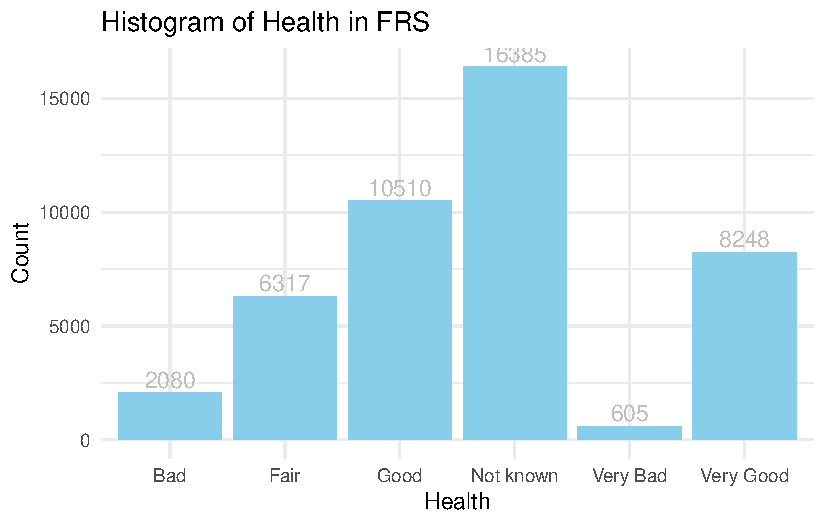
\includegraphics[keepaspectratio]{labs/03.QualitativeVariable_files/figure-pdf/unnamed-chunk-10-1.pdf}}

\begin{Shaded}
\begin{Highlighting}[]
\FunctionTok{ggplot}\NormalTok{(frs\_data, }\FunctionTok{aes}\NormalTok{(}\AttributeTok{x =}\NormalTok{ nssec)) }\SpecialCharTok{+} 
  \FunctionTok{geom\_bar}\NormalTok{(}\AttributeTok{fill =} \StringTok{"yellow4"}\NormalTok{) }\SpecialCharTok{+} 
  \FunctionTok{labs}\NormalTok{(}\AttributeTok{title =} \StringTok{"Histogram of NSSEC in FRS"}\NormalTok{, }\AttributeTok{x =} \StringTok{"NSSEC"}\NormalTok{, }\AttributeTok{y =} \StringTok{"Count"}\NormalTok{) }\SpecialCharTok{+}
  \FunctionTok{coord\_flip}\NormalTok{()}\SpecialCharTok{+} \CommentTok{\#Flip the Axes, add a \# in front of this line, to make the code in gray and you will see why we would better flip the axes at here}
  \FunctionTok{theme\_bw}\NormalTok{() }
\end{Highlighting}
\end{Shaded}

\pandocbounded{\includegraphics[keepaspectratio]{labs/03.QualitativeVariable_files/figure-pdf/unnamed-chunk-11-1.pdf}}

If we want to reorder the Y axis by from highest to lowest, we use the
functions in \texttt{forcats} library. \texttt{fct\_infreq()}: orders by
the value's frequency of the variable \texttt{nssec}.
\texttt{fct\_rev()}: reverses the order to go from highest to lowest.

\begin{Shaded}
\begin{Highlighting}[]
\FunctionTok{ggplot}\NormalTok{(frs\_data, }\FunctionTok{aes}\NormalTok{(}\AttributeTok{x =} \FunctionTok{fct\_rev}\NormalTok{(}\FunctionTok{fct\_infreq}\NormalTok{(nssec)))) }\SpecialCharTok{+} 
  \FunctionTok{geom\_bar}\NormalTok{(}\AttributeTok{fill =} \StringTok{"yellow4"}\NormalTok{) }\SpecialCharTok{+} 
  \FunctionTok{labs}\NormalTok{(}\AttributeTok{title =} \StringTok{"Histogram of NSSEC in FRS"}\NormalTok{, }\AttributeTok{x =} \StringTok{"NSSEC"}\NormalTok{, }\AttributeTok{y =} \StringTok{"Count"}\NormalTok{) }\SpecialCharTok{+}
  \FunctionTok{coord\_flip}\NormalTok{()}\SpecialCharTok{+} \CommentTok{\#Flip the Axes, add a \# in front of this line, to make the code in gray and you will see why we would better flip the axes at here}
  \FunctionTok{theme\_bw}\NormalTok{() }
\end{Highlighting}
\end{Shaded}

\pandocbounded{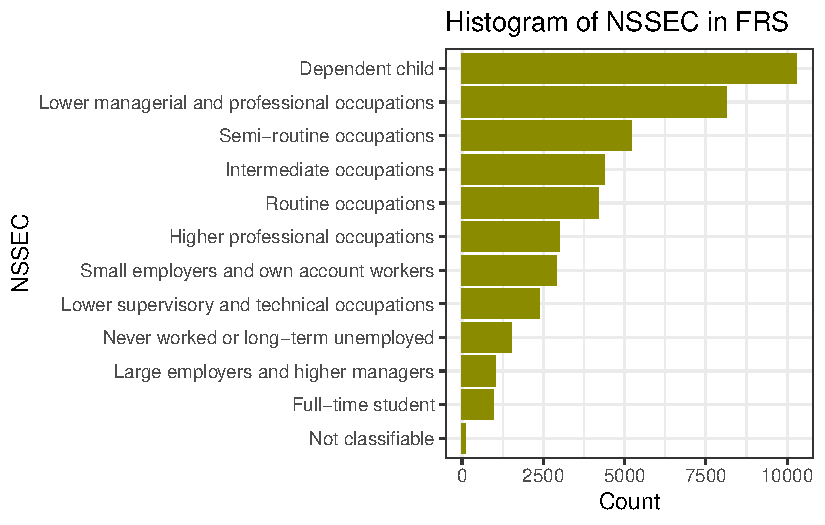
\includegraphics[keepaspectratio]{labs/03.QualitativeVariable_files/figure-pdf/unnamed-chunk-12-1.pdf}}

You can change the variables in ggplot() to make your own histogram
chart for the variables you are interested in. You will learn more of
visualisation methods in Week 5's practical.

\subsection{Correlation}\label{correlation}

\textbf{Q1. Which of the associations do you think is strongest? Which
is the weakest?}

As before, rather than relying upon an impressionistic view of the
strength of the association between two variables, we can measure that
association by calculating the relevant correlation coefficient.

To calculate the correlation between categorical data, we first use
Chi-squared test to assess the independence between pairs of categorical
variables, then we use Cramer's V to measures the strength of
association - the correlation coefficents in R.

\textbf{Pearson's chi-squared test} (χ2) is a statistical test applied
to sets of categorical data to evaluate how likely it is that any
observed difference between the sets arose by chance. If the p-value is
low (typically \textless{} 0.05), it suggests a significant association
between the two variables.

\begin{Shaded}
\begin{Highlighting}[]
\FunctionTok{chisq.test}\NormalTok{(frs\_data}\SpecialCharTok{$}\NormalTok{health,frs\_data}\SpecialCharTok{$}\NormalTok{happy) }
\end{Highlighting}
\end{Shaded}

\begin{verbatim}
Warning in chisq.test(frs_data$health, frs_data$happy): Chi-squared
approximation may be incorrect
\end{verbatim}

\begin{verbatim}

    Pearson's Chi-squared test

data:  frs_data$health and frs_data$happy
X-squared = 45594, df = 60, p-value < 2.2e-16
\end{verbatim}

If you see a warning message of Chi-squared approximation may be
incorrect. This is because some expected frequencies in one or more
cells of the cross-tabular (health * happy) are too low. The df means
degrees of freedom and it related to the size of the table and the
number of categories in each variable. The most important message from
the output is the estimated p-value, which shows as p-value \textless{}
2.2e-16 (2.2 with 16 decimals move to the left, it is a very small
number so written in scientific notation). P-value of the chi-squared
test is far smaller than 0.05, so we can say the correlation is
statistically significant.

\textbf{Cramér's V} is a measure of association for categorical (nominal
or ordinal) data. It ranges from 0 (no association) to 1 (strong
association). The main downside of using Cramer's V is that no
information is provided on whether the correlation is positive or
negative. This is not a problem if the variable pair includes a nominal
variable but represents an information loss if the both variables being
correlated are ordinal.

\begin{Shaded}
\begin{Highlighting}[]
\CommentTok{\# Install the \textquotesingle{}vcd\textquotesingle{} package if not installed }
\ControlFlowTok{if}\NormalTok{(}\SpecialCharTok{!}\FunctionTok{require}\NormalTok{(}\StringTok{"vcd"}\NormalTok{))   }
\FunctionTok{install.packages}\NormalTok{(}\StringTok{"vcd"}\NormalTok{, }\AttributeTok{repos =} \StringTok{"https://cran.r{-}project.org"}\NormalTok{, }\AttributeTok{dependencies =}\NormalTok{ T)}
\end{Highlighting}
\end{Shaded}

\begin{verbatim}
Loading required package: vcd
\end{verbatim}

\begin{verbatim}
Warning: package 'vcd' was built under R version 4.5.1
\end{verbatim}

\begin{verbatim}
Loading required package: grid
\end{verbatim}

\begin{Shaded}
\begin{Highlighting}[]
\FunctionTok{library}\NormalTok{(vcd)  }

\CommentTok{\# creat the crosstable }
\NormalTok{crosstab }\OtherTok{\textless{}{-}} \FunctionTok{table}\NormalTok{(frs\_data}\SpecialCharTok{$}\NormalTok{health, frs\_data}\SpecialCharTok{$}\NormalTok{happy)}

\CommentTok{\# Calculate Cramér\textquotesingle{}s V }
\FunctionTok{assocstats}\NormalTok{(crosstab)}
\end{Highlighting}
\end{Shaded}

\begin{verbatim}
                   X^2 df P(> X^2)
Likelihood Ratio 54036 60        0
Pearson          45594 60        0

Phi-Coefficient   : NA 
Contingency Coeff.: 0.713 
Cramer's V        : 0.454 
\end{verbatim}

\begin{Shaded}
\begin{Highlighting}[]
\CommentTok{\#you can also directly calculate the assoication between variables}
\FunctionTok{assocstats}\NormalTok{(}\FunctionTok{table}\NormalTok{(frs\_data}\SpecialCharTok{$}\NormalTok{health, frs\_data}\SpecialCharTok{$}\NormalTok{age\_group))}
\end{Highlighting}
\end{Shaded}

\begin{verbatim}
                   X^2 df P(> X^2)
Likelihood Ratio 26557 75        0
Pearson          23854 75        0

Phi-Coefficient   : NA 
Contingency Coeff.: 0.592 
Cramer's V        : 0.329 
\end{verbatim}

\textbf{Research Question 1. Which of our selected person-level
variables is most strongly correlated with an individual's health
status?}

Use the codes of Chi-test and Cramer's V to answer this question by
completing Table 1.

\textbf{Table 1 Person-level correlations with health status}

\begin{longtable}[]{@{}
  >{\raggedright\arraybackslash}p{(\linewidth - 6\tabcolsep) * \real{0.2500}}
  >{\raggedright\arraybackslash}p{(\linewidth - 6\tabcolsep) * \real{0.2500}}
  >{\raggedright\arraybackslash}p{(\linewidth - 6\tabcolsep) * \real{0.2500}}
  >{\raggedright\arraybackslash}p{(\linewidth - 6\tabcolsep) * \real{0.2500}}@{}}
\toprule\noalign{}
\endhead
\bottomrule\noalign{}
\endlastfoot
\textbf{Covariates} & & \textbf{Correlation Coefficient} &
\textbf{Statistical Significance} \\
& & \emph{Cramer's V} & \emph{p-value} \\
\emph{health} & \emph{age\_group} & & \\
\emph{Health} & \emph{highest\_qual} & & \\
\emph{health} & \emph{marital\_status} & & \\
\emph{Health} & \emph{nssec} & & \\
\end{longtable}

\section{Income inequality with respect to gender and health
status}\label{income-inequality-with-respect-to-gender-and-health-status}

In this section, we will work with individual-level data (``FRS
2016-17\_label.csv'') to explore income inequality with respect to
gender and health status.

To explore income inequality, we need to work with a data set excluding
dependent children. In addition, we look at individuals who are the
representative persons of households. Therefore, we will select cases
(or samples) that meet both conditions.

We want R to select persons only if they are the representative persons
of households and they are not dependent children. The involved
variables are \texttt{hrp} and \texttt{Dependent} for the categories
``Household Reference Person'' and ``independent'', you can select the
appropriate cases. We also want to exclude the health variable reported
as ``Not known''.

\begin{Shaded}
\begin{Highlighting}[]
\NormalTok{frs\_df }\OtherTok{\textless{}{-}}\NormalTok{ frs\_data }\SpecialCharTok{\%\textgreater{}\%} \FunctionTok{filter}\NormalTok{(hrp }\SpecialCharTok{==} \StringTok{"HRP"} \SpecialCharTok{\&}
\NormalTok{                                dependent }\SpecialCharTok{==} \StringTok{"Independent"} \SpecialCharTok{\&}
\NormalTok{                                health }\SpecialCharTok{!=} \StringTok{"Not known"}\NormalTok{) }
\end{Highlighting}
\end{Shaded}

Then, we create a new numeric variable \texttt{Net\_inc\_perc} indicate
net income per capita as our dependent variable:

\begin{Shaded}
\begin{Highlighting}[]
\NormalTok{frs\_df}\SpecialCharTok{$}\NormalTok{Net\_inc\_pp }\OtherTok{=}\NormalTok{ frs\_df}\SpecialCharTok{$}\NormalTok{hh\_income\_net }\SpecialCharTok{/}\NormalTok{ frs\_df}\SpecialCharTok{$}\NormalTok{hh\_size  }
\FunctionTok{summary}\NormalTok{(frs\_df}\SpecialCharTok{$}\NormalTok{Net\_inc\_pp)}
\end{Highlighting}
\end{Shaded}

\begin{verbatim}
   Min. 1st Qu.  Median    Mean 3rd Qu.    Max. 
-238160    9074   13347   15834   19136  864812 
\end{verbatim}

The distribution of the net household income per capita can be
visualised by using \texttt{ggplot()}

\begin{Shaded}
\begin{Highlighting}[]
\FunctionTok{ggplot}\NormalTok{(frs\_df, }\FunctionTok{aes}\NormalTok{(}\AttributeTok{x =}\NormalTok{ Net\_inc\_pp)) }\SpecialCharTok{+}
  \FunctionTok{geom\_histogram}\NormalTok{(}
    \AttributeTok{bins =} \DecValTok{250}\NormalTok{, }\CommentTok{\#A higher bins value means more, narrower bars, covers smaller range of value}
    \AttributeTok{color =} \StringTok{"black"}\NormalTok{,}
    \AttributeTok{fill =} \StringTok{"skyblue"}\NormalTok{,}
    \AttributeTok{alpha =} \FloatTok{0.7}
\NormalTok{  ) }\SpecialCharTok{+}   \FunctionTok{labs}\NormalTok{(}\AttributeTok{title =} \StringTok{"Distribution of Net\_inc\_pp"}\NormalTok{, }\AttributeTok{x =} \StringTok{"Value"}\NormalTok{, }\AttributeTok{y =}  \StringTok{"Frequency"}\NormalTok{) }\SpecialCharTok{+}   \FunctionTok{scale\_x\_continuous}\NormalTok{(}\AttributeTok{labels =}\NormalTok{ scales}\SpecialCharTok{::}\FunctionTok{label\_comma}\NormalTok{()) }\SpecialCharTok{+}  \CommentTok{\# Prevent scientific notation on the x axis}
  \FunctionTok{theme\_minimal}\NormalTok{()}
\end{Highlighting}
\end{Shaded}

\pandocbounded{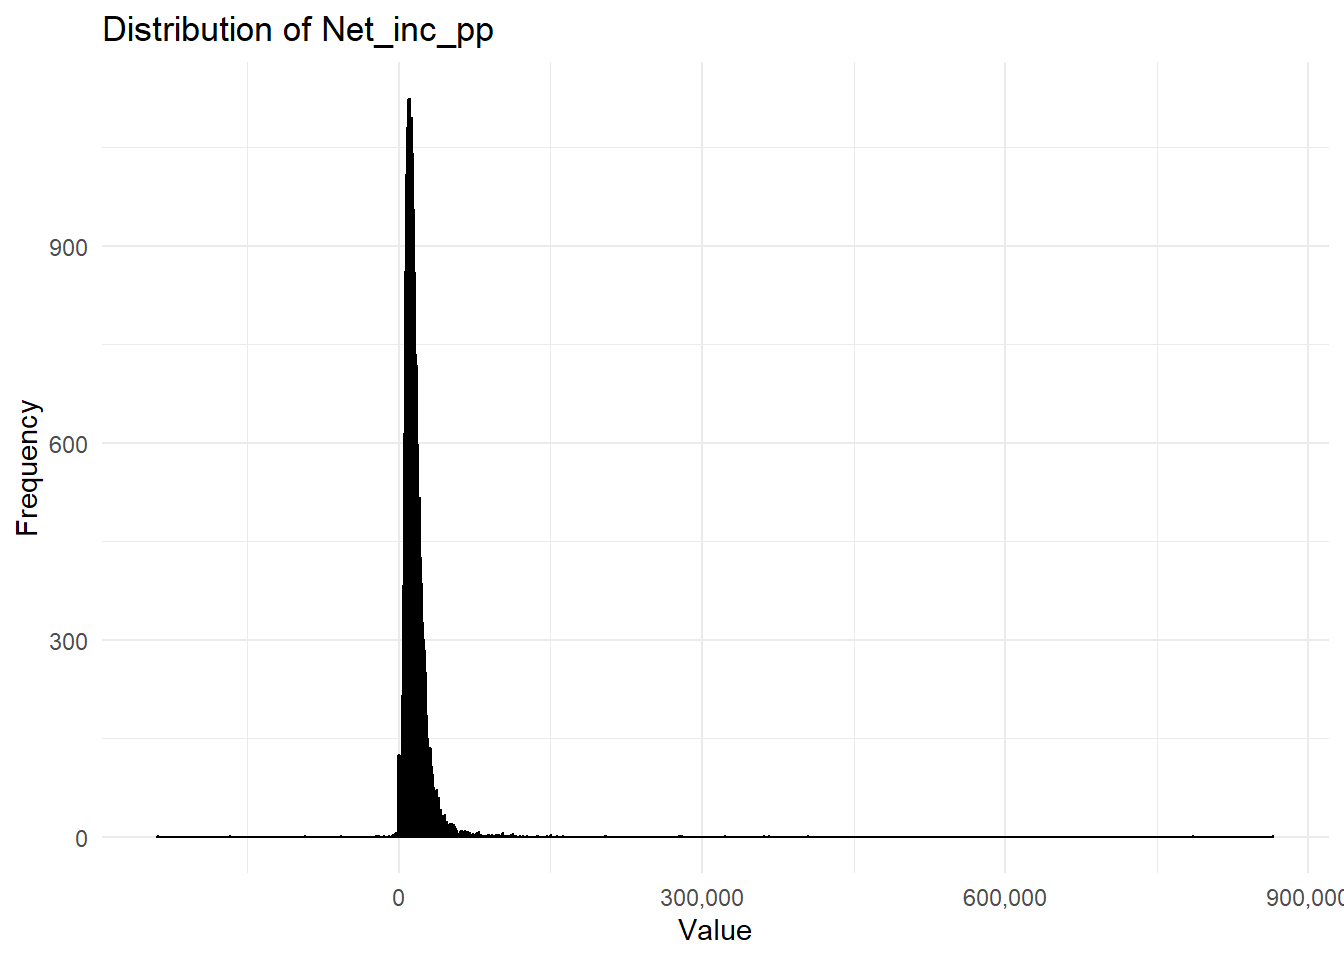
\includegraphics[keepaspectratio]{labs/03.QualitativeVariable_files/figure-pdf/unnamed-chunk-17-1.pdf}}

Our two qualitative independent variables ``\texttt{sex}'' and
``\texttt{health}''. Let's first know what they look like:

\begin{Shaded}
\begin{Highlighting}[]
\FunctionTok{table}\NormalTok{(frs\_df}\SpecialCharTok{$}\NormalTok{sex) }
\end{Highlighting}
\end{Shaded}

\begin{verbatim}

Female   Male 
  7647   9180 
\end{verbatim}

\begin{Shaded}
\begin{Highlighting}[]
\FunctionTok{table}\NormalTok{(frs\_df}\SpecialCharTok{$}\NormalTok{health)}
\end{Highlighting}
\end{Shaded}

\begin{verbatim}

      Bad      Fair      Good  Very Bad Very Good 
     1472      4253      6277       426      4399 
\end{verbatim}

Remember in the lecture, what we did in the Region long-term illness
before we put the categorical variable Region into the regression model?
Yes. First, make sure they are in factor type and Second, decide the
reference category. Here, I will use Female and Very Bad health status
as my base categories. You can decide what you wish to use. This time, I
use the following codes to combine these two steps in one line.

\begin{Shaded}
\begin{Highlighting}[]
\NormalTok{frs\_df}\SpecialCharTok{$}\NormalTok{sex }\OtherTok{\textless{}{-}} \FunctionTok{fct\_relevel}\NormalTok{(}\FunctionTok{as.factor}\NormalTok{(frs\_df}\SpecialCharTok{$}\NormalTok{sex), }\StringTok{"Female"}\NormalTok{) }
\NormalTok{frs\_df}\SpecialCharTok{$}\NormalTok{health }\OtherTok{\textless{}{-}} \FunctionTok{fct\_relevel}\NormalTok{(}\FunctionTok{as.factor}\NormalTok{(frs\_df}\SpecialCharTok{$}\NormalTok{health), }\StringTok{"Very Bad"}\NormalTok{)}
\end{Highlighting}
\end{Shaded}

Implement the regression model with the two qualitative independent
variables.

\begin{Shaded}
\begin{Highlighting}[]
\NormalTok{model\_frs }\OtherTok{\textless{}{-}} \FunctionTok{lm}\NormalTok{(Net\_inc\_pp }\SpecialCharTok{\textasciitilde{}}\NormalTok{ sex }\SpecialCharTok{+}\NormalTok{ health, }\AttributeTok{data =}\NormalTok{ frs\_df) }
\FunctionTok{summary}\NormalTok{(model\_frs)}
\end{Highlighting}
\end{Shaded}

\begin{verbatim}

Call:
lm(formula = Net_inc_pp ~ sex + health, data = frs_df)

Residuals:
    Min      1Q  Median      3Q     Max 
-255133   -6547   -2213    3515  845673 

Coefficients:
                Estimate Std. Error t value Pr(>|t|)    
(Intercept)      12115.5      762.9  15.881  < 2e-16 ***
sexMale           2091.2      240.6   8.691  < 2e-16 ***
healthBad         -102.8      854.3  -0.120 0.904205    
healthFair        1051.3      789.0   1.332 0.182751    
healthGood        2766.0      777.4   3.558 0.000375 ***
healthVery Good   4931.8      787.8   6.260 3.95e-10 ***
---
Signif. codes:  0 '***' 0.001 '**' 0.01 '*' 0.05 '.' 0.1 ' ' 1

Residual standard error: 15530 on 16821 degrees of freedom
Multiple R-squared:  0.01646,   Adjusted R-squared:  0.01616 
F-statistic: 56.29 on 5 and 16821 DF,  p-value: < 2.2e-16
\end{verbatim}

Same of what you have learnt in Week 2, the code explanation:

\textbf{\texttt{lm()} Function}:

\begin{itemize}
\tightlist
\item
  \texttt{lm()} stands for ``linear model'' and is used to fit a linear
  regression model in R.
\item
  The formula syntax
  \texttt{Net\_inc\_pp\ \textasciitilde{}\ Sex\ +\ health} specifies a
  relationship between:

  \begin{itemize}
  \tightlist
  \item
    \textbf{Dependent Variable}: \texttt{Net\_inc\_pp}.
  \item
    \textbf{Independent Variables}: \texttt{Sex}, and \texttt{health}.
    The model is trained on the \texttt{data\ =\ frs\_df} dataset.
  \end{itemize}
\end{itemize}

\textbf{Storing the Model}: The \texttt{model\ \textless{}-} syntax
stores the fitted model in an object called \texttt{model}.

\texttt{summary(model)} provides a detailed output of the model's
results, including:

\begin{itemize}
\tightlist
\item
  \textbf{Coefficients}: Estimates of the regression slopes (i.e., how
  each independent variableaffects \texttt{Net\_inc\_pp}).
\item
  \textbf{Standard Errors}: The variability of each coefficient
  estimate.
\item
  \textbf{t-values} and \textbf{p-values}: Indicate the statistical
  significance of the effect of each independent (explanatory) variable.
\item
  \textbf{R-squared} and \textbf{Adjusted R-squared}: Show how well the
  independent variables explain the variance in the dependent variable.
\item
  \textbf{F-statistic}: Tests the overall significance of the model.
\end{itemize}

The result can be formatted by:

\begin{Shaded}
\begin{Highlighting}[]
\FunctionTok{library}\NormalTok{(broom) }
\FunctionTok{tidy}\NormalTok{(model\_frs)}
\end{Highlighting}
\end{Shaded}

\begin{verbatim}
# A tibble: 6 x 5
  term            estimate std.error statistic  p.value
  <chr>              <dbl>     <dbl>     <dbl>    <dbl>
1 (Intercept)       12116.      763.    15.9   2.21e-56
2 sexMale            2091.      241.     8.69  3.90e-18
3 healthBad          -103.      854.    -0.120 9.04e- 1
4 healthFair         1051.      789.     1.33  1.83e- 1
5 healthGood         2766.      777.     3.56  3.75e- 4
6 healthVery Good    4932.      788.     6.26  3.95e-10
\end{verbatim}

\textbf{Q2.} \textbf{What conclusions could be drawn in terms of income
inequalities with respect to gender and health status? Also think about
the statistical significance of these differences.}

The interpretation of this table is again similar to what you have
learnt in Week2, but you may find that R has automatically treat your
categorical/qualitative variable Sex and Health as dummy variables, so
in the output, you see sexMale, the reason there is no sexFemale is
because I requested R to use sex=Female as the reference category. You
also wee healthBad, healthFair, healthGood, and healthVery Good, but you
didn't see health Very Bad because agaion I request
\texttt{frs\_df\$health\ \textless{}-\ fct\_relevel(as.factor(frs\_df\$health),\ "Very\ Bad")}
.

For the independent variable, the coefficient estimates of them need to
be interpreted by comparing to the reference category: Male and Very Bad
health. We can derive how the differences between different independent
variable categories are associated with the changes in
\texttt{Net\_inc\_pp}, for example:

\begin{itemize}
\tightlist
\item
  The association of \texttt{sexMale}is positive and strong: compare to
  sex=Female, \texttt{sexMale} is associated with an increase of £2,091
  net income per capita, here we see some gender inequality;
\item
  The association of \texttt{healthBad} and \texttt{healthFair} arenot
  statistically significant, which means we cannot draw any conclusion
  of the relationships between \texttt{healthBad} and
  \texttt{Net\_inc\_pp} or \texttt{healthFair} and \texttt{Net\_inc\_pp}
  from the model ;
\item
  Then, the association of \texttt{healthGood} and
  \texttt{healthVeryGood} are both positive and strong:
  \texttt{healthGood} is associated with an increase of £2,766 net
  income per capita compared to \texttt{healthVeryBad}, and
  \texttt{healthVeryGood} is associated with an increase of £4,931 net
  income per capita compared to \texttt{healthVeryBad} . Here you may
  draw some useful conclusion on who the health condition impact the
  inequality of income.
\end{itemize}

We then read R-squared and Adjusted R-squared to evaluate the model fit.
We see both values are only around 0.016, which means in the model
\texttt{Net\_inc\_pp\ \textasciitilde{}\ Sex\ +\ health} , the
independent variable \texttt{Sex\ +\ health} can only explain 1.6\% of
the variation of our dependent variable \texttt{Net\_inc\_pp}. This is a
relatively poor performance, and the model cannot be used to do any
prediction of \texttt{Net\_inc\_pp} by using just sex and health. This
also suggests us that to fully explain the \texttt{Net\_inc\_pp} , we
may need to add in more variables, such as education level, occupation,
age, etc. Although the model is not solid for any prediction, the
coefficients and significant conclusion from the model are still very
useful.

\section{\texorpdfstring{\textbf{Implementing a linear regression model
with a qualitative independent
variable}}{Implementing a linear regression model with a qualitative independent variable}}\label{implementing-a-linear-regression-model-with-a-qualitative-independent-variable}

To gain further practice on using linear regression model with
qualitative variables as independent variables, we follow the model you
created last week, to add in the qualitative/categorical variable Region
from the Census 2021 dataset. You should already have the dataset
\textbf{EW\_DistrictPercentages.csv}, if not, you can download them from
\href{https://canvas.liverpool.ac.uk/courses/84668/pages/census-data?module_item_id=2396199}{Canvas}.
Please put the .csv file in you `/data/Census2021' folder.

\textbf{Research Question 2: How does health vary across regions in the
UK?}

The practical is split into two main parts. The first focuses on
implementing a linear regression model with a qualitative independent
variable. \textbf{Note that} you need first to set the reference
category (baseline) as the outcomes of the model reflects the
\textbf{differences} between categories with the baseline. The second
part focuses prediction based the estimated linear regression model.

First we load the UK district-level census dataset.

\begin{Shaded}
\begin{Highlighting}[]
\CommentTok{\# load data}
\NormalTok{LAcensus }\OtherTok{\textless{}{-}} \FunctionTok{read.csv}\NormalTok{(}\StringTok{"../data/Census2021/EW\_DistrictPercentages.csv"}\NormalTok{) }\CommentTok{\# Local authority level}
\end{Highlighting}
\end{Shaded}

Using the district-level census dataset
``\textbf{EW\_\_DistrictPercentages.csv}''. the variable ``Region''
(labelled as Government Office Region) is used to explore regional
inequality in health.

Familiar yourself with the dataset by using the same codes as last week:

\begin{Shaded}
\begin{Highlighting}[]
\CommentTok{\#view the data }
\FunctionTok{View}\NormalTok{(LAcensus)  }
\FunctionTok{glimpse}\NormalTok{(LAcensus)}
\end{Highlighting}
\end{Shaded}

The names() function returns all the column names.

\begin{Shaded}
\begin{Highlighting}[]
\FunctionTok{names}\NormalTok{(LAcensus)}
\end{Highlighting}
\end{Shaded}

The dim() function can merely returns the number of rows and number of
columns.

\begin{Shaded}
\begin{Highlighting}[]
\FunctionTok{dim}\NormalTok{(LAcensus) }
\end{Highlighting}
\end{Shaded}

\begin{verbatim}
[1] 331 161
\end{verbatim}

There are 331 rows and 151 columns in the dataset. It would be very hard
to scan throught the data if we use so many variables altogether.
Therefore, we can select several columns to tailor for this practical.
You can of course include other variables you are interested in also by
their names:

\begin{Shaded}
\begin{Highlighting}[]
\NormalTok{df }\OtherTok{\textless{}{-}}\NormalTok{ LAcensus }\SpecialCharTok{\%\textgreater{}\%} \FunctionTok{select}\NormalTok{(}\FunctionTok{c}\NormalTok{(}\StringTok{"pct\_Longterm\_sick\_or\_disabled"}\NormalTok{,}
                            \StringTok{"pct\_No\_qualifications"}\NormalTok{,}
                            \StringTok{"pct\_Males"}\NormalTok{,}
                            \StringTok{"pct\_Higher\_manager\_prof"}\NormalTok{,}
                            \StringTok{"Region"}\NormalTok{))}
\end{Highlighting}
\end{Shaded}

Simply descriptive of this new data

\begin{Shaded}
\begin{Highlighting}[]
\FunctionTok{summary}\NormalTok{(df)}
\end{Highlighting}
\end{Shaded}

\begin{verbatim}
 pct_Longterm_sick_or_disabled pct_No_qualifications   pct_Males    
 Min.   :1.330                 Min.   : 6.61         Min.   :46.77  
 1st Qu.:2.865                 1st Qu.:15.06         1st Qu.:48.62  
 Median :3.810                 Median :17.63         Median :48.98  
 Mean   :4.013                 Mean   :17.90         Mean   :48.97  
 3rd Qu.:4.800                 3rd Qu.:20.41         3rd Qu.:49.30  
 Max.   :9.110                 Max.   :28.88         Max.   :55.02  
 pct_Higher_manager_prof    Region         
 Min.   : 5.49           Length:331        
 1st Qu.: 9.79           Class :character  
 Median :12.34           Mode  :character  
 Mean   :13.22                             
 3rd Qu.:15.80                             
 Max.   :39.68                             
\end{verbatim}

Now we can retrieve the ``Region'' column from the data frame by simply
use \textbf{df\$Region}. But what if we want to understand the data
better, like the following questions?

\textbf{Q3. How many categories do the variable ``Region'' entail? How
many local authority districts does each region include?}

Simply use the function table() would return you the answer.

\begin{Shaded}
\begin{Highlighting}[]
\FunctionTok{table}\NormalTok{(df}\SpecialCharTok{$}\NormalTok{Region) }
\end{Highlighting}
\end{Shaded}

\begin{verbatim}

                    East            East Midlands                   London 
                      45                       35                       33 
              North East               North West               South East 
                      12                       39                       64 
              South West                    Wales            West Midlands 
                      30                       22                       30 
Yorkshire and The Humber 
                      21 
\end{verbatim}

The \texttt{table()} function tells us that this data frame contains 10
regions, and the number of LAs belongs to each region.

**R can only include the categorical variables in the \textbf{factor}
type, so we set the column \emph{Region} in \texttt{factor()}

\begin{Shaded}
\begin{Highlighting}[]
\NormalTok{df}\SpecialCharTok{$}\NormalTok{Region}\OtherTok{\textless{}{-}} \FunctionTok{factor}\NormalTok{(df}\SpecialCharTok{$}\NormalTok{Region) }
\end{Highlighting}
\end{Shaded}

\subsection{\texorpdfstring{\textbf{Include the categorical variables
into a regression
model}}{Include the categorical variables into a regression model}}\label{include-the-categorical-variables-into-a-regression-model}

We will continue with a very similar regression model fitted in last
week that relates Percentages long-term illness
(\emph{pct\_Long\_term\_sick\_or\_disabled}) to Percentages
no-qualification (\emph{pct\_No\_qualifications}), Percentage Males
(\emph{pct\_Males}) and Percentages Higher Managerial or Professional
occupation (\emph{pct\_Higher\_manager\_prof}).

Decide which region to be set as the baseline category. The principle is
that if you want to compare the (average) long term illness outcome of
Region A to those of other regions, Region A should be chosen as the
baseline category. For example, if you want to compare the (average)
long term illness outcome of London to rest of regions in the England
and Wales, London should be selected as the baseline category.

Implement the regression model with the categorical variables -
\emph{Region} in our case. R will automatically handle the qualitative
variable as dummy variables so you don't need to concern any of that.
But you need to let R knows which category of your qualitative variable
is your reference category or the baseline. Here we will use London as
our first go. \textbf{Note:} We choose London as the baseline category
so the London region will be \ul{\textbf{excluded}} in the independent
variable list.

Therefore, first, we set London as the reference:

\begin{Shaded}
\begin{Highlighting}[]
\NormalTok{df}\SpecialCharTok{$}\NormalTok{Region }\OtherTok{\textless{}{-}} \FunctionTok{fct\_relevel}\NormalTok{(df}\SpecialCharTok{$}\NormalTok{Region,  }\StringTok{"London"}\NormalTok{)}
\end{Highlighting}
\end{Shaded}

Similar to last week, we build our linear regression model, but also
include the \emph{Region} variable into the model.

\begin{Shaded}
\begin{Highlighting}[]
\NormalTok{model }\OtherTok{\textless{}{-}} \FunctionTok{lm}\NormalTok{(pct\_Longterm\_sick\_or\_disabled }\SpecialCharTok{\textasciitilde{}}\NormalTok{ pct\_Males }\SpecialCharTok{+}\NormalTok{ pct\_No\_qualifications }\SpecialCharTok{+}\NormalTok{ pct\_Higher\_manager\_prof }\SpecialCharTok{+}\NormalTok{ Region, }\AttributeTok{data =}\NormalTok{ df)}

\FunctionTok{summary}\NormalTok{(model)}
\end{Highlighting}
\end{Shaded}

\begin{verbatim}

Call:
lm(formula = pct_Longterm_sick_or_disabled ~ pct_Males + pct_No_qualifications + 
    pct_Higher_manager_prof + Region, data = df)

Residuals:
     Min       1Q   Median       3Q      Max 
-1.73799 -0.42623 -0.08528  0.41308  2.20676 

Coefficients:
                                Estimate Std. Error t value Pr(>|t|)    
(Intercept)                     7.615375   3.018425   2.523  0.01212 *  
pct_Males                      -0.167291   0.061638  -2.714  0.00701 ** 
pct_No_qualifications           0.251334   0.023179  10.843  < 2e-16 ***
pct_Higher_manager_prof         0.007145   0.020244   0.353  0.72438    
RegionEast                     -0.760329   0.173260  -4.388 1.56e-05 ***
RegionEast Midlands            -0.254826   0.194419  -1.311  0.19090    
RegionNorth East                1.164153   0.260808   4.464 1.12e-05 ***
RegionNorth West                0.784897   0.192449   4.078 5.74e-05 ***
RegionSouth East               -0.328575   0.165728  -1.983  0.04827 *  
RegionSouth West                0.096484   0.214507   0.450  0.65317    
RegionWales                     1.382217   0.220643   6.264 1.21e-09 ***
RegionWest Midlands            -0.415570   0.196345  -2.117  0.03508 *  
RegionYorkshire and The Humber -0.118795   0.217473  -0.546  0.58528    
---
Signif. codes:  0 '***' 0.001 '**' 0.01 '*' 0.05 '.' 0.1 ' ' 1

Residual standard error: 0.7086 on 318 degrees of freedom
Multiple R-squared:  0.7593,    Adjusted R-squared:  0.7502 
F-statistic:  83.6 on 12 and 318 DF,  p-value: < 2.2e-16
\end{verbatim}

You have already learnt how to interpret the output of regression model
last week: \textbf{Significance} (p-value), \textbf{Coefficient
Estimates, and Model fit} (R squared and Adjusted R-squared).

\textbf{Q4. Relating back to this week's lecture notes, indicate what
regions have statistically significant differences in the percentage of
long-term illness, compared to London?}

First, the \textbf{Significance} and the \textbf{Coefficient Estimates}.
By examining the P-value, which is the last column in the output table,
we can see that most of the independent variables are significant
predictor of \texttt{pct\_Longterm\_sick\_or\_disabled}.

\begin{itemize}
\item
  Similarly to last week, we learn that the changes in
  \texttt{pct\_No\_qualifications} are significantly associated with
  changes in \texttt{pct\_Longterm\_sick\_or\_disabled} at the
  \textless0.001 level (with the three asterisks *** ), which is
  actually an indicator of highly statistically significant, while we
  are less confident that the observed relationship between
  \texttt{pct\_No\_qualifications} and
  \texttt{pct\_Longterm\_sick\_or\_disabled} are statistically
  significant (with the two asterisks **). Through their coefficient
  estimates, we learn that:

  \begin{itemize}
  \item
    The association of \texttt{pct\_Males} is negative and mild: each
    decrease in 1\% of \texttt{pct\_Males} is associated with an
    increase of 0.17\% of long term sick/disable rate in the population
    of EW.
  \item
    The association of \texttt{pct\_No\_qualifications} is positive and
    strong: each increase in 1\% of \texttt{pct\_No\_qualifications} is
    associated with an increase of 0.25\% of long term sick/disable
    rate.
  \item
    The association of \texttt{pct\_Higher\_manager\_prof} is not
    statistically significant.
  \end{itemize}
\item
  Now comes to the dummy variables (all the items starts with Region)
  created by R for our qualitative variable \emph{Region}:
  \texttt{RegionEast}, \texttt{RegionNorth\ Eest},
  \texttt{RegionNorth\ West} and \texttt{RegionWales} are also
  statistically significant at the \textless0.001 level. The changes in
  \texttt{RegionSouth\ East} and \texttt{RegionWest\ Midlands} are
  significantly associated with changes in
  \texttt{pct\_Longterm\_sick\_or\_disabled} at the 0.05 level. The 0.05
  level suggests that it is a mild likelihood that the relationship
  between these independent variables and the dependent variable is not
  due to random change. They are just mildly statistically significant.
\item
  The coefficient estimates of them need to be interpreted by comparing
  to the reference category London. The Estimate column tells us: North
  East region is associated with a 1.16\% higher rate of long term
  sick/disable than London when the other predictors remain the same.
  Similarly, Wales is 1.38\% higher rate of long term illness than
  London when the other predictors remain the same. You can draw the
  conclusion for the other regions in this way by using their
  coefficient estimate values.

  \textbf{Reminder}: You \textbf{cannot} draw conclusion between North
  East and Wales, nor comparison between any regions beyond London. It
  is because the regression model is built for the comparison between
  regions to your reference category London. If we want to compare
  between North East and Wales, we need to set either of them as the
  reference category by using
  \texttt{df\$Region\ \textless{}-\ fct\_relevel(df\$Region,\ "North\ East")}
  or
  \texttt{df\$Region\ \textless{}-\ fct\_relevel(df\$Region,\ "Wales")}.
\item
  \texttt{RegionEast\ Midland}, \texttt{RegionSouth\ West}, and
  \texttt{RegionlYorkshire\ and\ The\ Humber} were not found to be
  significantly associated with
  \texttt{pct\_Longterm\_sick\_or\_disabled}.
\end{itemize}

Last but not least, the \textbf{Measure of Model Fit}. The model output
suggests the R-squared and Adjusted R-squared are of greater than 0.75
indicate a reasonably well fitting model. The model explains 75.9 \% of
the variance in the dependent variable. After adjusting for the number
of independent variable, the model explains 75.0\% of the variance. They
two suggest a strong fit of the model.

\subsection{\texorpdfstring{\textbf{Change the baseline
category}}{Change the baseline category}}\label{change-the-baseline-category}

If you would like to learn about differences in long-term illness
between North East and other regions in the EW, you need to change the
baseline category (from London) to the North East region (with variable
name ``Region\_2'').

\begin{Shaded}
\begin{Highlighting}[]
\NormalTok{df}\SpecialCharTok{$}\NormalTok{Region }\OtherTok{\textless{}{-}} \FunctionTok{fct\_relevel}\NormalTok{(df}\SpecialCharTok{$}\NormalTok{Region, }\StringTok{"North West"}\NormalTok{)}
\end{Highlighting}
\end{Shaded}

The regression model is specified again as follows:

\begin{Shaded}
\begin{Highlighting}[]
\NormalTok{model1 }\OtherTok{\textless{}{-}} \FunctionTok{lm}\NormalTok{(}
\NormalTok{  pct\_Longterm\_sick\_or\_disabled }\SpecialCharTok{\textasciitilde{}}\NormalTok{ pct\_Males }\SpecialCharTok{+}\NormalTok{ pct\_No\_qualifications }\SpecialCharTok{+}\NormalTok{ pct\_Higher\_manager\_prof }\SpecialCharTok{+}\NormalTok{ Region,}
  \AttributeTok{data =}\NormalTok{ df}
\NormalTok{)}

\FunctionTok{summary}\NormalTok{(model1)}
\end{Highlighting}
\end{Shaded}

\begin{verbatim}

Call:
lm(formula = pct_Longterm_sick_or_disabled ~ pct_Males + pct_No_qualifications + 
    pct_Higher_manager_prof + Region, data = df)

Residuals:
     Min       1Q   Median       3Q      Max 
-1.73799 -0.42623 -0.08528  0.41308  2.20676 

Coefficients:
                                Estimate Std. Error t value Pr(>|t|)    
(Intercept)                     8.400272   3.042017   2.761 0.006090 ** 
pct_Males                      -0.167291   0.061638  -2.714 0.007009 ** 
pct_No_qualifications           0.251334   0.023179  10.843  < 2e-16 ***
pct_Higher_manager_prof         0.007145   0.020244   0.353 0.724376    
RegionLondon                   -0.784897   0.192449  -4.078 5.74e-05 ***
RegionEast                     -1.545226   0.158845  -9.728  < 2e-16 ***
RegionEast Midlands            -1.039723   0.165225  -6.293 1.03e-09 ***
RegionNorth East                0.379256   0.235090   1.613 0.107685    
RegionSouth East               -1.113472   0.152463  -7.303 2.27e-12 ***
RegionSouth West               -0.688413   0.182460  -3.773 0.000192 ***
RegionWales                     0.597320   0.189607   3.150 0.001786 ** 
RegionWest Midlands            -1.200467   0.174076  -6.896 2.89e-11 ***
RegionYorkshire and The Humber -0.903692   0.191943  -4.708 3.74e-06 ***
---
Signif. codes:  0 '***' 0.001 '**' 0.01 '*' 0.05 '.' 0.1 ' ' 1

Residual standard error: 0.7086 on 318 degrees of freedom
Multiple R-squared:  0.7593,    Adjusted R-squared:  0.7502 
F-statistic:  83.6 on 12 and 318 DF,  p-value: < 2.2e-16
\end{verbatim}

Examining R-squared to measure the model fit. How robust is the new
model? What \% of the variance in the dependent variable has been
explained?

Now, complete the following table.

\begin{longtable}[]{@{}
  >{\centering\arraybackslash}p{(\linewidth - 4\tabcolsep) * \real{0.3333}}
  >{\centering\arraybackslash}p{(\linewidth - 4\tabcolsep) * \real{0.3333}}
  >{\centering\arraybackslash}p{(\linewidth - 4\tabcolsep) * \real{0.3333}}@{}}
\toprule\noalign{}
\begin{minipage}[b]{\linewidth}\centering
Region names
\end{minipage} & \begin{minipage}[b]{\linewidth}\centering
Higher or lower than North West
\end{minipage} & \begin{minipage}[b]{\linewidth}\centering
Whether the difference is statistically significant (Yes or No)
\end{minipage} \\
\midrule\noalign{}
\endhead
\bottomrule\noalign{}
\endlastfoot
East Midlands & & \\
East of England & & \\
North East & & \\
North West & & \\
South East & & \\
London & & \\
West Midlands & & \\
Yorkshire and The Humber & & \\
Wales & & \\
\end{longtable}

Now it is very easy to use your model to estimate the results Y
(dependent variable - \texttt{pct\_Longterm\_sick\_or\_disabled} ) by
setting all the input independent variable X (\texttt{pct\_Males}
\texttt{pct\_No\_qualifications} and
\texttt{pct\_Higher\_manager\_prof}).

\begin{Shaded}
\begin{Highlighting}[]
\NormalTok{obj\_London }\OtherTok{\textless{}{-}} \FunctionTok{data.frame}\NormalTok{(}
  \AttributeTok{pct\_Males =} \FloatTok{49.7}\NormalTok{,}
  \AttributeTok{pct\_No\_qualifications =} \FloatTok{24.3}\NormalTok{,}
  \AttributeTok{pct\_Higher\_manager\_prof =} \FloatTok{14.7}\NormalTok{,}
  \AttributeTok{Region =} \StringTok{"London"}
\NormalTok{) }
\NormalTok{obj\_WM }\OtherTok{\textless{}{-}} \FunctionTok{data.frame}\NormalTok{(}
  \AttributeTok{pct\_Males =} \FloatTok{49.8}\NormalTok{,}
  \AttributeTok{pct\_No\_qualifications =} \FloatTok{23.3}\NormalTok{,}
  \AttributeTok{pct\_Higher\_manager\_prof =} \FloatTok{11.2}\NormalTok{,}
  \AttributeTok{Region =} \StringTok{"West Midlands"}
\NormalTok{) }
\NormalTok{obj\_NE }\OtherTok{\textless{}{-}} \FunctionTok{data.frame}\NormalTok{(}
  \AttributeTok{pct\_Males =} \FloatTok{49.8}\NormalTok{,}
  \AttributeTok{pct\_No\_qualifications =} \FloatTok{23.3}\NormalTok{,}
  \AttributeTok{pct\_Higher\_manager\_prof =} \FloatTok{11.2}\NormalTok{,}
  \AttributeTok{Region =} \StringTok{"North East"}
  
\NormalTok{) }

\FunctionTok{predict}\NormalTok{(model1, obj\_London) }
\end{Highlighting}
\end{Shaded}

\begin{verbatim}
       1 
5.513467 
\end{verbatim}

\begin{Shaded}
\begin{Highlighting}[]
\FunctionTok{predict}\NormalTok{(model1, obj\_WM) }
\end{Highlighting}
\end{Shaded}

\begin{verbatim}
       1 
4.804829 
\end{verbatim}

\begin{Shaded}
\begin{Highlighting}[]
\FunctionTok{predict}\NormalTok{(model1, obj\_NE)}
\end{Highlighting}
\end{Shaded}

\begin{verbatim}
       1 
6.384552 
\end{verbatim}

\subsection{Recode the Region variable and explore regional inequality
in
health}\label{recode-the-region-variable-and-explore-regional-inequality-in-health}

In many real-word studies, we might not be interested in health
inequality across all regions. For example, in this case study, we are
interested in health inequality between \emph{London}, \emph{South,
North, Midland and Wales}. We can achieve this by re-grouping regions in
the UK based on the variable ``Region''. That said, we need to have a
new grouping of regions as follows:

\begin{longtable}[]{@{}ll@{}}
\toprule\noalign{}
\endhead
\bottomrule\noalign{}
\endlastfoot
\textbf{Original region labels} & \textbf{New region labels} \\
East Midlands & Midlands \\
East & South \\
London & London \\
North East & North \\
North West & North \\
South East & South \\
South West & South \\
West Midlands & Midlands \\
Yorkshire and The Humber & North \\
Wales & Wales \\
\end{longtable}

Here we use mutate() function in R to make it happen:

\begin{Shaded}
\begin{Highlighting}[]
\NormalTok{df }\OtherTok{\textless{}{-}}\NormalTok{ df }\SpecialCharTok{\%\textgreater{}\%}
  \FunctionTok{mutate}\NormalTok{(}
    \AttributeTok{New\_region\_label =} \FunctionTok{fct\_collapse}\NormalTok{(}
\NormalTok{      Region,}
      \AttributeTok{North =} \FunctionTok{c}\NormalTok{(}\StringTok{"North East"}\NormalTok{, }\StringTok{"North West"}\NormalTok{, }\StringTok{"Yorkshire and The Humber"}\NormalTok{),}
      \AttributeTok{Midlands =} \FunctionTok{c}\NormalTok{(}\StringTok{"East Midlands"}\NormalTok{, }\StringTok{"West Midlands"}\NormalTok{),}
      \AttributeTok{South =} \FunctionTok{c}\NormalTok{(}\StringTok{"East"}\NormalTok{, }\StringTok{"South East"}\NormalTok{, }\StringTok{"South West"}\NormalTok{),}
      \AttributeTok{London =} \StringTok{"London"}\NormalTok{,}
      \AttributeTok{Wales =} \StringTok{"Wales"}
\NormalTok{    )}
\NormalTok{  )}
\end{Highlighting}
\end{Shaded}

This code may looks a bit complex. You can simply type ?mutate in your
console. Now in your right hand Help window, the R studio offers your
the explanation of the mutate function. This is a common way you can use
R studio to help you learn what the function ca\texttt{ate()} creates
new columns that are functions of existing variables. Therefore, the
\texttt{df\ \%\textgreater{}\%\ mutate()} means add a new column into
the current dataframe \texttt{df}; the \texttt{New\_region\_label} in
the \texttt{mutate()} function indicates the name of this new column is
\texttt{New\_region\_label}. The right side of the
\texttt{New\_region\_label\ =} indicates the value we want to assign to
the \texttt{New\_region\_label} in each row.

The right side of \texttt{New\_region\_label} is

\texttt{fct\_collapse(Region,\ North\ =\ c("North\ East",\ "North\ West",\ "Yorkshire\ and\ The\ Humber"),\ Midlands\ =\ c("East\ Midlands",\ "West\ Midlands"),\ South\ =\ c("East",\ "South\ East",\ "South\ West"),\ London\ =\ "London",\ Wales\ =\ "Wales")}

By using the code, the \texttt{fct\_collapse()} function recodes or
group each value in the \texttt{Region} column into one of the broader
categories: ``London'', ``South'', ``North'',``Midlands'' or ``Wales''.
Specifically, it takes the existing factor levels in \texttt{Region} and
collapses multiple detailed regions into fewer, aggregated groups. For
example, regions such as \emph{``North East''}, \emph{``North West''},
and \emph{``Yorkshire and The Humber''} are all grouped under
\textbf{``North''}, while \emph{``East Midlands''} and \emph{``West
Midlands''} are combined into \textbf{``Midlands''}, and so on.

Now we use the same way to examine our new column
\texttt{New\_region\_label}:

\begin{Shaded}
\begin{Highlighting}[]
\FunctionTok{table}\NormalTok{(df}\SpecialCharTok{$}\NormalTok{New\_region\_label)}
\end{Highlighting}
\end{Shaded}

\begin{verbatim}

   North   London    South Midlands    Wales 
      72       33      139       65       22 
\end{verbatim}

Comparing with the \texttt{Region\_label}, we now can see the mutate
worked:

\begin{Shaded}
\begin{Highlighting}[]
\NormalTok{df[,}\FunctionTok{c}\NormalTok{(}\StringTok{"Region"}\NormalTok{,}\StringTok{"New\_region\_label"}\NormalTok{)]}
\end{Highlighting}
\end{Shaded}

Now you will have a new qualitative variable named
\texttt{New\_region\_label} in which the UK is divided into four
regions: London, South, North and Midlands.

\emph{Based on the newly generated qualitative variable}
\texttt{New\_region\_label}, we can now build our new linear regression
model. Don't forget:

(1) R need to deal with the categorical variables in regression model in
the factor type;

\begin{Shaded}
\begin{Highlighting}[]
\FunctionTok{class}\NormalTok{(df}\SpecialCharTok{$}\NormalTok{New\_region\_label)}
\end{Highlighting}
\end{Shaded}

\begin{verbatim}
[1] "factor"
\end{verbatim}

The \texttt{class()} returns the type of the variable. The
\texttt{New\_region\_label} is already a factor variable. If not, we
need to convert it by the \texttt{as.factor()}, as we used above.

\begin{Shaded}
\begin{Highlighting}[]
\NormalTok{df}\SpecialCharTok{$}\NormalTok{New\_region\_label }\OtherTok{=} \FunctionTok{as.factor}\NormalTok{(df}\SpecialCharTok{$}\NormalTok{New\_region\_label)}
\end{Highlighting}
\end{Shaded}

2) Let R know which region you want to use as the baseline category.
Here I will use London again, but of course you can choose other
regions.

\begin{Shaded}
\begin{Highlighting}[]
\NormalTok{df}\SpecialCharTok{$}\NormalTok{New\_region\_label }\OtherTok{\textless{}{-}} \FunctionTok{fct\_relevel}\NormalTok{(df}\SpecialCharTok{$}\NormalTok{New\_region\_label, }\StringTok{"London"}\NormalTok{)}
\end{Highlighting}
\end{Shaded}

The linear regression window is set up below. This time we include
\texttt{New\_region\_label} rather than \texttt{Region\_label} as the
region variable:

\begin{Shaded}
\begin{Highlighting}[]
\NormalTok{model2 }\OtherTok{\textless{}{-}} \FunctionTok{lm}\NormalTok{(}
\NormalTok{  pct\_Longterm\_sick\_or\_disabled }\SpecialCharTok{\textasciitilde{}}\NormalTok{ pct\_Males }\SpecialCharTok{+}\NormalTok{ pct\_No\_qualifications }\SpecialCharTok{+}\NormalTok{ pct\_Higher\_manager\_prof }\SpecialCharTok{+}\NormalTok{ New\_region\_label,}
  \AttributeTok{data =}\NormalTok{ df}
\NormalTok{)}

\FunctionTok{summary}\NormalTok{(model2)}
\end{Highlighting}
\end{Shaded}

\begin{verbatim}

Call:
lm(formula = pct_Longterm_sick_or_disabled ~ pct_Males + pct_No_qualifications + 
    pct_Higher_manager_prof + New_region_label, data = df)

Residuals:
     Min       1Q   Median       3Q      Max 
-1.83271 -0.48362 -0.06293  0.40581  2.11961 

Coefficients:
                         Estimate Std. Error t value Pr(>|t|)    
(Intercept)               9.98363    3.20535   3.115  0.00201 ** 
pct_Males                -0.18418    0.06585  -2.797  0.00547 ** 
pct_No_qualifications     0.20143    0.02257   8.924  < 2e-16 ***
pct_Higher_manager_prof  -0.03410    0.01986  -1.718  0.08684 .  
New_region_labelNorth     0.47416    0.18706   2.535  0.01172 *  
New_region_labelSouth    -0.50635    0.16433  -3.081  0.00224 ** 
New_region_labelMidlands -0.41031    0.18517  -2.216  0.02740 *  
New_region_labelWales     1.25183    0.23431   5.343 1.73e-07 ***
---
Signif. codes:  0 '***' 0.001 '**' 0.01 '*' 0.05 '.' 0.1 ' ' 1

Residual standard error: 0.76 on 323 degrees of freedom
Multiple R-squared:  0.7188,    Adjusted R-squared:  0.7127 
F-statistic:   118 on 7 and 323 DF,  p-value: < 2.2e-16
\end{verbatim}

\textbf{Q5. Are there statistically significant differences in the
percentage of people with long-term sick/disable between London and
North, and between South and Wales, controlling for other variables?
What conclusions could be drawn in terms of regional differences in
health outcome?}

\section{Predictions using fitted regression
model}\label{predictions-using-fitted-regression-model}

\textbf{Write down the \% long term sick or disabled regression model
with the new region label categorical variables.}

Relating to this week's lecture, the \%
\texttt{pct\_Longterm\_sick\_or\_disabled} is equal to:

\textbf{{[}write down the model{]}}

\textbf{Q6. Now imagine that the values of variables \emph{pct\_Males,
pct\_No\_qualifications, and pct\_Higher\_manager\_prof} are 49, 23 and
11, respectively, what would the percentage of persons with long-term
sick/disable in Wales and London be?}

Check the answer at the end of this practical page.

\section{\texorpdfstring{\textbf{Extension
activities}}{Extension activities}}\label{extension-activities}

The extension activities are designed to get yourself prepared for the
Assignment 1 in progress. For this week, try whether you can:

\begin{itemize}
\item
  Present descriptive statistics for independent variable and the
  dependent variable: counts, percentages, a centrality measure, a
  spread measure, histograms or any relevant statistic
\item
  Report the observed association between the dependent and independent
  variables: correlation plus a graphic or tabular visualisation
\item
  Briefly describe and critically discuss the results
\item
  Think about other potential factors of long-term illness and income,
  and then test your ideas with linear regression models
\item
  Summaries your model outputs and interpret the results.
\end{itemize}

\section{\texorpdfstring{\textbf{Answer of the written down model and
Q6}}{Answer of the written down model and Q6}}\label{answer-of-the-written-down-model-and-q6}

The model of the new region label is:
\emph{pct\_Longterm\_sick\_or\_disabled} (\%) \emph{= 9.98+ (-0.1842)*
pct\_Males} (\%) \emph{+ 0.2014 * pct\_No\_qualifications} (\%) \emph{+
(-0.0341) * pct\_Higher\_manager\_prof} + \emph{(0.4742) * North +
(-0.5063)} * South + (-0.4103) * Midlands + \emph{1.2518 * Wales.} But
should be aware that the relation between
\emph{pct\_Higher\_manager\_prof} and
\emph{pct\_Longterm\_sick\_or\_disabled} is not statistically
significant.

So if the values of variables \emph{pct\_Males, pct\_No\_qualifications,
and pct\_Higher\_manager\_prof} are 49, 23 and 11,

the model of Wales will be: \emph{pct\_Longterm\_sick\_or\_disabled}
(\%) \emph{= 9.98+ (-0.1842)* 49} \emph{+ 0.2014 * 23} \emph{+ (-0.0341)
* 11 + (0.4742) * 0+ (-0.5063)} * 0+ (-0.4103) * 0+ \emph{1.2518 *
1}(you can direct paste the number sentence into your R studio Console
and the result will be returned)

the model of London will be: \emph{pct\_Long\_term\_ill} (\%) \emph{=
9.98+ (-0.1842)* 49} \emph{+ 0.2014 * 23} \emph{+ (-0.0341) * 11 +
(0.4742) * 0+ (-0.5063)} * 0+ (-0.4103) * 0+ \emph{1.2518 * 0}

You can also make a new object like

\begin{Shaded}
\begin{Highlighting}[]
\NormalTok{obj\_Wales }\OtherTok{\textless{}{-}} \FunctionTok{data.frame}\NormalTok{(}
  \AttributeTok{pct\_Males =} \DecValTok{49}\NormalTok{,}
  \AttributeTok{pct\_No\_qualifications =} \DecValTok{23}\NormalTok{,}
  \AttributeTok{pct\_Higher\_manager\_prof =} \DecValTok{11}\NormalTok{,}
  \AttributeTok{New\_region\_label =} \StringTok{"Wales"}
\NormalTok{)}

\NormalTok{obj\_London }\OtherTok{\textless{}{-}} \FunctionTok{data.frame}\NormalTok{(}
  \AttributeTok{pct\_Males =} \DecValTok{49}\NormalTok{,}
  \AttributeTok{pct\_No\_qualifications =} \DecValTok{23}\NormalTok{,}
  \AttributeTok{pct\_Higher\_manager\_prof =} \DecValTok{11}\NormalTok{,}
  \AttributeTok{New\_region\_label =} \StringTok{"London"}
\NormalTok{)}

\FunctionTok{predict}\NormalTok{(model2, obj\_Wales)}
\end{Highlighting}
\end{Shaded}

\begin{verbatim}
       1 
6.468668 
\end{verbatim}

\begin{Shaded}
\begin{Highlighting}[]
\FunctionTok{predict}\NormalTok{(model2, obj\_London)}
\end{Highlighting}
\end{Shaded}

\begin{verbatim}
       1 
5.216834 
\end{verbatim}

\textbf{Therefore, the percentage of persons with long-term illness in
Wales and London be 6.47\% and 5.22 \% and separately. If you got the
right answers, then congratulations you can now use regression model to
make prediction.}

\bookmarksetup{startatroot}

\chapter{Lab: Logistic Regression}\label{lab-logistic-regression}

Last week, we learnt how to use qualitative variables in multiple linear
regression model to understand the relationship between independent
variables X1 \ldots{} Xn and the dependent variable Y. Today we will
learn to use logistic regression for binary dependent variable. A
\textbf{logistic regression model} is a type of regression analysis used
when the dependent variable is binary (e.g., ``success/failure'' or
``0/1''). It estimates the probability of one outcome relative to the
other using a logistic function. This model is commonly used in
situations like predicting disease presence (yes/no) or customer churn
(stay/leave). The independent variables can be continuous, categorical,
or a mix of both. The model's output is in the form of odds ratios,
showing how predictors affect the likelihood of the outcome.

The lecture's slides can be
found~\href{https://github.com/GDSL-UL/stats/blob/main/lectures/lecture04.pdf}{here}.

\textbf{Learning objectives}

An understanding of, and ability to:

\begin{itemize}
\item
  Estimate and interpret a logistic regression model
\item
  Assess the model fit
\end{itemize}

The application context of a binomial logistic regression model is when
the dependent variable under investigation is a binary variable.
Usually, a value of 1 for this dependent variable means the occurrence
of an event; and, 0 otherwise. For example, the dependent variable for
this practical is whether a person is a long-distance commuter i.e.~1,
and 0 otherwise.

In this week's practical, we are going to apply logistic regression
analysis in an attempt to answer the following research question:

\textbf{RESEARCH QUESTION: Who is willing to commute long distances?}

The practical is split into two main parts. The first focuses on
implementing a binary logistic regression model with R. The second part
focuses the interpretation of the resulting estimates.

\section{Knowing the dataset and descriptive
analysis}\label{knowing-the-dataset-and-descriptive-analysis}

Prepare the data for implementing a logistic regression model. The data
set used in this practical is the ``sar\_sample\_label.csv'' and
``sar\_sample\_code.csv''. The SAR is a snapshot of census microdata,
which are individual level data. The data sample has been drawn and
anonymised from census and known as the Samples of Anonymised Records
(SARs).

You may need to download the two datasets and also the data dictionary
from
\href{https://canvas.liverpool.ac.uk/courses/84668/pages/sample-of-anonymised-records-sar-dataset?module_item_id=2422237}{Canvas}
if you haven't. Double click to open both .csv files you may find they
have exactly same column names - yes, they are in fact the same
spreadsheet but `sar\_sample\_label.csv' is more readable for the cell
contents as they are in text format but cells in the
`sar\_sample\_code.csv' is in coding format. The `SAR\_dictionary' is
create to help you understand what the columns mean, just like the FRS
dictionary for the FRS datasets last week. Yes, the two SAR csv files
are actually the same dataframe, only one uses the label as the value
but the other uses the code. This is quite normal as when we doing
surveys, we use text as the options of multiple choice questions for
respondents to choose from, and therefore the collected survey results
are in the `sar\_sample\_label' format. The label format is usually more
readable and is good to do descriptive analysis as we will show in
today's content. However, we may find the coding format is more concise
for writing the code and thus will be used during regression analysis.
\textbf{Please notice that coding the labels into numbers, doesn't mean
the categorical/qualitative variable has been converted into
numeric/continuous numbers.}

Let's first read in both for the data overview.

\begin{Shaded}
\begin{Highlighting}[]
\ControlFlowTok{if}\NormalTok{(}\SpecialCharTok{!}\FunctionTok{require}\NormalTok{(}\StringTok{"tidyverse"}\NormalTok{))}
  \FunctionTok{install.packages}\NormalTok{(}\StringTok{"tidyverse"}\NormalTok{,}\AttributeTok{dependencies =}\NormalTok{ T, }\AttributeTok{repos =} \StringTok{"https://cloud.r{-}project.org/"}\NormalTok{)}
\end{Highlighting}
\end{Shaded}

\begin{verbatim}
Warning: package 'tidyverse' was built under R version 4.5.1
\end{verbatim}

\begin{verbatim}
Warning: package 'ggplot2' was built under R version 4.5.1
\end{verbatim}

\begin{verbatim}
Warning: package 'tibble' was built under R version 4.5.1
\end{verbatim}

\begin{verbatim}
Warning: package 'tidyr' was built under R version 4.5.1
\end{verbatim}

\begin{verbatim}
Warning: package 'readr' was built under R version 4.5.1
\end{verbatim}

\begin{verbatim}
Warning: package 'purrr' was built under R version 4.5.1
\end{verbatim}

\begin{verbatim}
Warning: package 'dplyr' was built under R version 4.5.1
\end{verbatim}

\begin{verbatim}
Warning: package 'forcats' was built under R version 4.5.1
\end{verbatim}

\begin{verbatim}
Warning: package 'lubridate' was built under R version 4.5.1
\end{verbatim}

\begin{Shaded}
\begin{Highlighting}[]
\ControlFlowTok{if}\NormalTok{(}\SpecialCharTok{!}\FunctionTok{require}\NormalTok{(}\StringTok{"broom"}\NormalTok{))}
  \FunctionTok{install.packages}\NormalTok{(}\StringTok{"broom"}\NormalTok{,}\AttributeTok{dependencies =}\NormalTok{ T, }\AttributeTok{repos =} \StringTok{"https://cloud.r{-}project.org/"}\NormalTok{)}
\end{Highlighting}
\end{Shaded}

\begin{verbatim}
Warning: package 'broom' was built under R version 4.5.1
\end{verbatim}

\begin{Shaded}
\begin{Highlighting}[]
\ControlFlowTok{if}\NormalTok{(}\SpecialCharTok{!}\FunctionTok{require}\NormalTok{(}\StringTok{"forcats"}\NormalTok{))}
  \FunctionTok{install.packages}\NormalTok{(}\StringTok{"forcats"}\NormalTok{)}

\FunctionTok{library}\NormalTok{(tidyverse)}
\FunctionTok{library}\NormalTok{(broom)}
\FunctionTok{library}\NormalTok{(forcats)}
\end{Highlighting}
\end{Shaded}

\begin{Shaded}
\begin{Highlighting}[]
\NormalTok{sar\_label }\OtherTok{\textless{}{-}} \FunctionTok{read.csv}\NormalTok{(}\StringTok{"../data/SAR/sar\_sample\_label.csv"}\NormalTok{)}
\NormalTok{sar\_code }\OtherTok{\textless{}{-}} \FunctionTok{read.csv}\NormalTok{(}\StringTok{"../data/SAR/sar\_sample\_code.csv"}\NormalTok{)}
\end{Highlighting}
\end{Shaded}

Run the following codes to view both dataframes:

\begin{Shaded}
\begin{Highlighting}[]
\CommentTok{\#View the sar\_label dataset}
\FunctionTok{View}\NormalTok{(sar\_label)}
\end{Highlighting}
\end{Shaded}

\begin{Shaded}
\begin{Highlighting}[]
\CommentTok{\#View the sar\_code dataset}
\FunctionTok{View}\NormalTok{(sar\_code)}
\end{Highlighting}
\end{Shaded}

To know the dataset better, we can run dim() to know who many
individuals (rows) in this sample data and how many variables (columns)
have been recorded.

\begin{Shaded}
\begin{Highlighting}[]
\FunctionTok{dim}\NormalTok{(sar\_label)}
\end{Highlighting}
\end{Shaded}

\begin{verbatim}
[1] 50000    39
\end{verbatim}

\begin{Shaded}
\begin{Highlighting}[]
\CommentTok{\#or}
\FunctionTok{dim}\NormalTok{(sar\_code)}
\end{Highlighting}
\end{Shaded}

\begin{verbatim}
[1] 50000    39
\end{verbatim}

So there are 50,000 respondents in the sample dataset and 39 variables
are included.

After browsing both data sheets and also the data dictionary (sometimes
we call it meta data), you may notice that all the columns in the SAR
dataset is categorical/qualitative type. Therefore, if we run the
\texttt{summary()} function for the dataframes, as we did in previous
weeks for the Census data or the FRS dataset, the outputs of the
\texttt{summary()} may not be very useful. Again, please notice that the
figures in the sar\_code.csv is not mean actual numbers, but the codes
of different categories of the qualitative variables. Therefore, the
\texttt{summary()} results at there is not useful. Please reflect what
we've learnt in last week's, when the variables if
categorical/qualitative type, how we do the descriptive analysis for
them?

\begin{Shaded}
\begin{Highlighting}[]
\FunctionTok{summary}\NormalTok{(sar\_code)}
\FunctionTok{summary}\NormalTok{(sar\_label)}
\end{Highlighting}
\end{Shaded}

So, the answer is we focus on summarising the frequency and distribution
of categories within the variable and the function in R for doing this
is \texttt{table()}. For example, the variable ``work\_distance''
captures a person's commuting distance. We can run the table() for both
label and code csv to understand the distribution, composition and
diversity of categories of the '\,'work\_distance'' in the data. Try to
repeat what we have learnt in Week 3 to finish the \textbf{descriptive
analysis} for the categorical variables in SAR (by ggplot2).

\begin{Shaded}
\begin{Highlighting}[]
\FunctionTok{table}\NormalTok{(sar\_label}\SpecialCharTok{$}\NormalTok{work\_distance)}
\end{Highlighting}
\end{Shaded}

\begin{verbatim}

                                10 to <20 km 
                                        3650 
                                  2 to <5 km 
                                        4414 
                                20 to <40 km 
                                        2014 
                                 40 to <60km 
                                         572 
                                 5 to <10 km 
                                        4190 
                                60km or more 
                                         703 
                       Age<16 or not working 
                                       25975 
                                     At home 
                                        2427 
                              Less than 2 km 
                                        4028 
                              No fixed place 
                                        1943 
Work outside England and Wales but within UK 
                                          29 
                             Work outside UK 
                                          21 
  Works at offshore installation (within UK) 
                                          34 
\end{verbatim}

\begin{Shaded}
\begin{Highlighting}[]
\FunctionTok{table}\NormalTok{(sar\_code}\SpecialCharTok{$}\NormalTok{work\_distance)}
\end{Highlighting}
\end{Shaded}

\begin{verbatim}

   -9     1     2     3     4     5     6     7     8     9    10    11    12 
25975  4028  4414  4190  3650  2014   572   703  2427  1943    29    21    34 
\end{verbatim}

To create a chart as part of the descriptive analysis, exactly as what
we did in Week 3, we use the library ggplots and the codes:

\begin{Shaded}
\begin{Highlighting}[]
\FunctionTok{library}\NormalTok{(ggplot2)}
\FunctionTok{ggplot}\NormalTok{(sar\_label, }\FunctionTok{aes}\NormalTok{(}\AttributeTok{x =}\NormalTok{ work\_distance)) }\SpecialCharTok{+} 
  \FunctionTok{geom\_bar}\NormalTok{(}\AttributeTok{fill =} \StringTok{"rosybrown"}\NormalTok{) }\SpecialCharTok{+} 
  \FunctionTok{labs}\NormalTok{(}\AttributeTok{title =} \StringTok{"Histogram of work distrance in SAR sample"}\NormalTok{, }\AttributeTok{x =} \StringTok{"Work Distance"}\NormalTok{, }\AttributeTok{y =} \StringTok{"Count"}\NormalTok{) }\SpecialCharTok{+}
  \FunctionTok{coord\_flip}\NormalTok{()}\SpecialCharTok{+} \CommentTok{\#Flip the Axes, add a \# in front of this line, to make the code in gray and you will see why we would better flip the axes at here}
  \FunctionTok{theme\_bw}\NormalTok{() }
\end{Highlighting}
\end{Shaded}

\pandocbounded{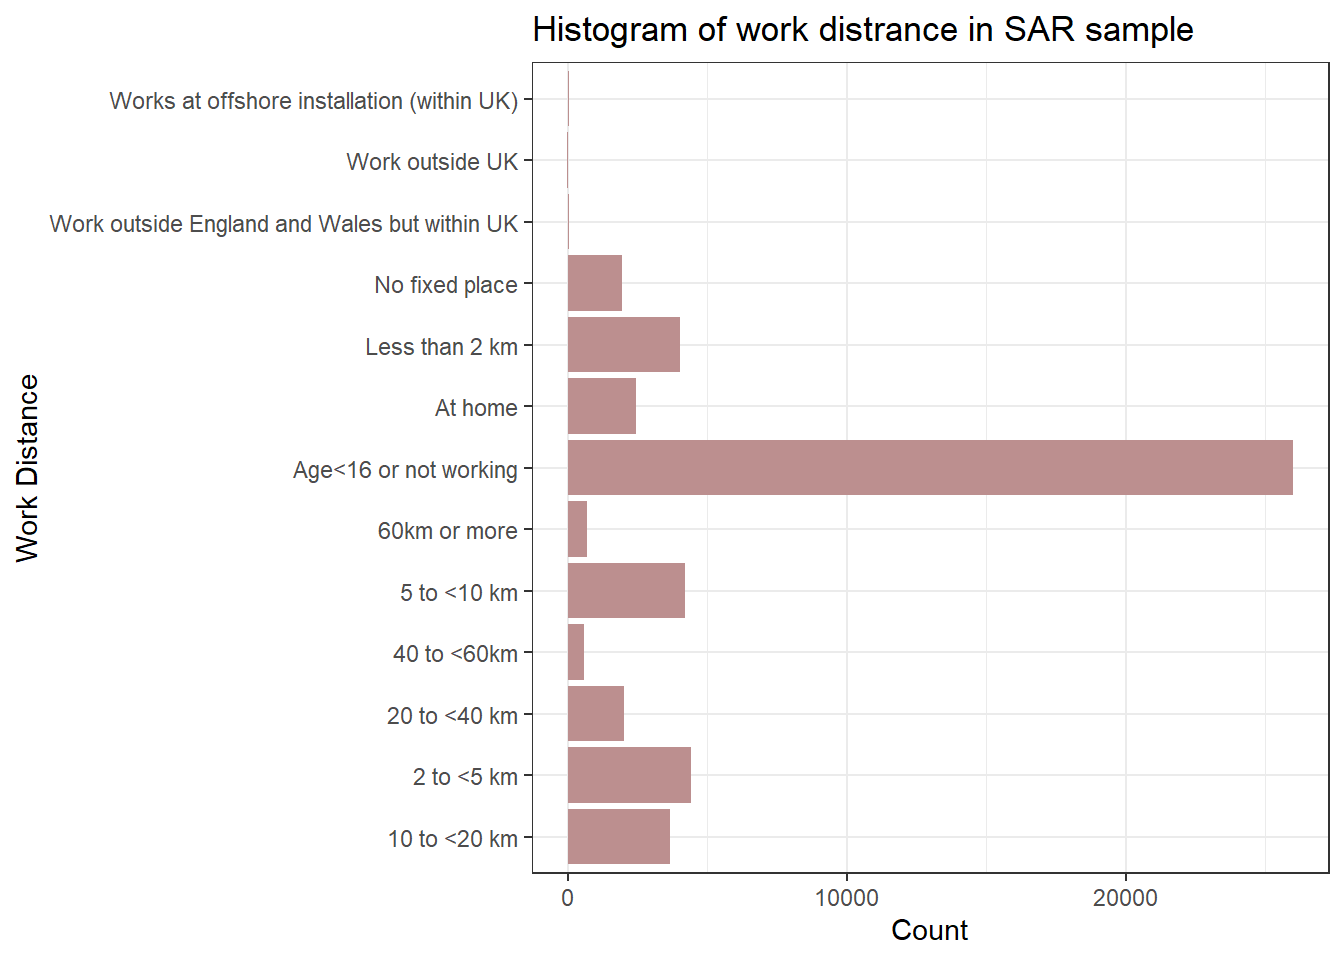
\includegraphics[keepaspectratio]{labs/04.LogisticRegression_files/figure-pdf/unnamed-chunk-8-1.pdf}}

We have learnt that for the categorical/qualitative variables, we need R
to treat them as \texttt{factor} type. Therefore, if we want to create
descriptive analysis charts by using \texttt{sar\_code} , we need first
convert the code numbers from numeric to factor type.

\begin{Shaded}
\begin{Highlighting}[]
\FunctionTok{library}\NormalTok{(ggplot2)}
\FunctionTok{ggplot}\NormalTok{(sar\_code, }\FunctionTok{aes}\NormalTok{(}\AttributeTok{x =} \FunctionTok{as.factor}\NormalTok{(work\_distance))) }\SpecialCharTok{+} 
  \FunctionTok{geom\_bar}\NormalTok{(}\AttributeTok{fill =} \StringTok{"rosybrown"}\NormalTok{) }\SpecialCharTok{+} 
  \FunctionTok{labs}\NormalTok{(}\AttributeTok{title =} \StringTok{"Histogram of work distrance in SAR sample"}\NormalTok{, }\AttributeTok{x =} \StringTok{"Work Distance"}\NormalTok{, }\AttributeTok{y =} \StringTok{"Count"}\NormalTok{) }\SpecialCharTok{+}
  \FunctionTok{coord\_flip}\NormalTok{()}\SpecialCharTok{+} \CommentTok{\#Flip the Axes, add a \# in front of this line, to make the code in gray and you will see why we would better flip the axes at here}
  \FunctionTok{theme\_bw}\NormalTok{() }
\end{Highlighting}
\end{Shaded}

\pandocbounded{\includegraphics[keepaspectratio]{labs/04.LogisticRegression_files/figure-pdf/unnamed-chunk-9-1.pdf}}

You may also realise that this chart is not that readable to be used as
a descriptive analysis chart to put in the report as the Y-axis are all
in codes, therefore the first chart created by labels is a better
choice. Based on `SAR\_dictionary.xlsx', we learn how the codes map to
the categories for the variable work\_distance in both csv.

\begin{longtable}[]{@{}
  >{\raggedright\arraybackslash}p{(\linewidth - 2\tabcolsep) * \real{0.3429}}
  >{\raggedright\arraybackslash}p{(\linewidth - 2\tabcolsep) * \real{0.6571}}@{}}
\toprule\noalign{}
\begin{minipage}[b]{\linewidth}\raggedright
Code for Work\_distance
\end{minipage} & \begin{minipage}[b]{\linewidth}\raggedright
Categories
\end{minipage} \\
\midrule\noalign{}
\endhead
\bottomrule\noalign{}
\endlastfoot
-9 & Age\textless16 or not working \\
1 & Less than 2 km \\
2 & 2 to \textless5 km \\
3 & 5 to \textless10 km \\
4 & 10 to \textless20 km \\
5 & 20 to \textless40 km \\
6 & 40 to \textless60 km \\
7 & 60km or more \\
8 & At home \\
9 & No fixed place \\
10 & Work outside England and Wales but within UK \\
11 & Work outside UK \\
12 & Works at offshore installation (within UK) \\
\end{longtable}

There are a variety of categories in the variable, however, we are only
interested in commuting distance and therefore in people reporting their
commuting distance. \textbf{Thus, we will explore the numeric codes of
the variable ranging from 1 to 8.}

As we are also interested in exploring whether people with different
socio-economic statuses (or occupations) tend to be associated with
varying probabilities of commuting over long distances, we further
filter or select cases.

\begin{Shaded}
\begin{Highlighting}[]
\FunctionTok{table}\NormalTok{(sar\_label}\SpecialCharTok{$}\NormalTok{nssec)}
\end{Highlighting}
\end{Shaded}

\begin{verbatim}

                              Child aged 0-15 
                                         9698 
                            Full-time student 
                                         3041 
              Higher professional occupations 
                                         3162 
                     Intermediate occupations 
                                         5288 
          Large employers and higher managers 
                                          909 
Lower managerial and professional occupations 
                                         8345 
  Lower supervisory and technical occupations 
                                         2924 
         Never worked or long-term unemployed 
                                         2261 
                          Routine occupations 
                                         4660 
                     Semi-routine occupations 
                                         5893 
      Small employers and own account workers 
                                         3819 
\end{verbatim}

\begin{Shaded}
\begin{Highlighting}[]
\FunctionTok{table}\NormalTok{(sar\_code}\SpecialCharTok{$}\NormalTok{nssec)}
\end{Highlighting}
\end{Shaded}

\begin{verbatim}

   1    2    3    4    5    6    7    8    9   10   12 
 909 3162 8345 5288 3819 2924 5893 4660 2261 3041 9698 
\end{verbatim}

\begin{Shaded}
\begin{Highlighting}[]
\FunctionTok{ggplot}\NormalTok{(sar\_label, }\FunctionTok{aes}\NormalTok{(}\AttributeTok{x =} \FunctionTok{fct\_rev}\NormalTok{(}\FunctionTok{fct\_infreq}\NormalTok{(nssec)))) }\SpecialCharTok{+} 
  \FunctionTok{geom\_bar}\NormalTok{(}\AttributeTok{fill =} \StringTok{"tan"}\NormalTok{) }\SpecialCharTok{+} 
  \FunctionTok{labs}\NormalTok{(}\AttributeTok{title =} \StringTok{"Histogram of NSSEC in SAR sample"}\NormalTok{, }\AttributeTok{x =} \StringTok{"NSSEC"}\NormalTok{, }\AttributeTok{y =} \StringTok{"Count"}\NormalTok{) }\SpecialCharTok{+}
  \FunctionTok{coord\_flip}\NormalTok{()}\SpecialCharTok{+} \CommentTok{\#Flip the Axes, add a \# in front of this line, to make the code in gray and you will see why we would better flip the axes at here}
  \FunctionTok{theme\_bw}\NormalTok{() }
\end{Highlighting}
\end{Shaded}

\pandocbounded{\includegraphics[keepaspectratio]{labs/04.LogisticRegression_files/figure-pdf/unnamed-chunk-11-1.pdf}}

From `SAR\_dictionary.xlsx', we learn what each code indicate
corresponding category for variable \texttt{nssec}. For the following
regression model, we select people who reported an occupation, and
delete cases with numeric codes from 9 to 12, who are \emph{unemployed},
\emph{full-time students}, \emph{children} and \emph{not classifiable}.

\begin{longtable}[]{@{}ll@{}}
\toprule\noalign{}
Code for nssec & Category labels \\
\midrule\noalign{}
\endhead
\bottomrule\noalign{}
\endlastfoot
1 & Large employers and higher managers \\
2 & Higher professional occupations \\
3 & Lower managerial and professional occupations \\
4 & Intermediate occupations \\
5 & Small employers and own account workers \\
6 & Lower supervisory and technical occupations \\
7 & Semi-routine occupations \\
8 & Routine occupations \\
9 & Never worked or long-term employed \\
10 & Full-time student \\
11 & Not classifiable \\
12 & Child aged 0-15 \\
\end{longtable}

Now, similar to next week, we use the \texttt{filter()} to prepare our
dataframe today. You may already realise that using \texttt{sar\_code}
is easier to do the filtering.

\begin{Shaded}
\begin{Highlighting}[]
\NormalTok{sar\_df }\OtherTok{\textless{}{-}}\NormalTok{ sar\_code }\SpecialCharTok{\%\textgreater{}\%} \FunctionTok{filter}\NormalTok{(work\_distance}\SpecialCharTok{\textless{}=}\DecValTok{8} \SpecialCharTok{\&}\NormalTok{ nssec }\SpecialCharTok{\textless{}=}\DecValTok{8}\NormalTok{ )}
\end{Highlighting}
\end{Shaded}

\textbf{Q1. Create descriptive analysis for the two variables
``work\_distance'', ``nssec'' and ``sex'' with the new data, including
(1) summarise the frequencies and (2) create histogram charts for the
three variables.}

\section{Preparing the input
variables}\label{preparing-the-input-variables}

For a logistic regression model, we first need to \textbf{recode the
``work\_distance'' variable into a binary dependent variable} as our
independent variable.

A simple way to create a binary dependent variable representing
long-distance commuting is to use the mutate() function as discussed in
last week's practical session. Before creating the binary variables from
the ``work\_distance'' variable, we need to define \emph{what counts as
a long-distance commuting move}. Such definition can vary. Here we
define a long-distance commuting move as any commuting move over a
distance above 60km (the category of ``60km or more'').

\begin{Shaded}
\begin{Highlighting}[]
\NormalTok{sar\_df }\OtherTok{\textless{}{-}}\NormalTok{ sar\_df }\SpecialCharTok{\%\textgreater{}\%} \FunctionTok{mutate}\NormalTok{(}
  \AttributeTok{New\_work\_distance =} \FunctionTok{if\_else}\NormalTok{(work\_distance }\SpecialCharTok{\textgreater{}}\DecValTok{6}\NormalTok{, }\DecValTok{1}\NormalTok{,}\DecValTok{0}\NormalTok{))}
\end{Highlighting}
\end{Shaded}

\textbf{Q2.} \textbf{Do descripitve analysis to the new \texttt{sar\_df}
dataframe with new column named \texttt{New\_work\_distance} by using
the codes you have learnt.}

The independent variables are gender and socio-economic status. The
gender variable \texttt{sex} is a categorical variable. Therefore, as
we've learnt last week, before adding the categorical variables into the
regression model, we need first make it a factor and then identify the
reference category. For gender, we use male as the basline. Prepare your
``sex'' variable before the regression model:

\begin{Shaded}
\begin{Highlighting}[]
\NormalTok{sar\_df}\SpecialCharTok{$}\NormalTok{sex }\OtherTok{\textless{}{-}} \FunctionTok{relevel}\NormalTok{(}\FunctionTok{as.factor}\NormalTok{(sar\_df}\SpecialCharTok{$}\NormalTok{sex),}\AttributeTok{ref=}\StringTok{"1"}\NormalTok{)}
\end{Highlighting}
\end{Shaded}

Then, we prepare socio-economic status variable \texttt{nssec} for the
regression model. We are interested in whether people with occupations
being ``Higher professional occupations'' are associated with a lower
probability of commuting over long distances when comparing to people in
other occupations. Therefore by using the ``Higher professional
occupations'' code 2, we run the code as below:

\begin{Shaded}
\begin{Highlighting}[]
\NormalTok{sar\_df}\SpecialCharTok{$}\NormalTok{nssec }\OtherTok{\textless{}{-}} \FunctionTok{relevel}\NormalTok{(}\FunctionTok{as.factor}\NormalTok{(sar\_df}\SpecialCharTok{$}\NormalTok{nssec), }\AttributeTok{ref =} \StringTok{"2"}\NormalTok{)}
\end{Highlighting}
\end{Shaded}

\section{\texorpdfstring{\textbf{Implementing a logistic regression
model}}{Implementing a logistic regression model}}\label{implementing-a-logistic-regression-model}

The binary dependent variable is long-distance commuting, variable name
\texttt{New\_work\_distance}.

\begin{Shaded}
\begin{Highlighting}[]
\CommentTok{\#create the model}
\NormalTok{m.glm }\OtherTok{=} \FunctionTok{glm}\NormalTok{(New\_work\_distance}\SpecialCharTok{\textasciitilde{}}\NormalTok{sex }\SpecialCharTok{+}\NormalTok{ nssec, }
            \AttributeTok{data =}\NormalTok{ sar\_df, }
            \AttributeTok{family=} \StringTok{"binomial"}\NormalTok{)}
\CommentTok{\# inspect the results}
\FunctionTok{summary}\NormalTok{(m.glm) }
\end{Highlighting}
\end{Shaded}

\begin{verbatim}

Call:
glm(formula = New_work_distance ~ sex + nssec, family = "binomial", 
    data = sar_df)

Coefficients:
            Estimate Std. Error z value Pr(>|z|)    
(Intercept) -1.67337    0.05329 -31.401  < 2e-16 ***
sex2        -0.36678    0.04196  -8.742  < 2e-16 ***
nssec1      -0.12881    0.11306  -1.139    0.255    
nssec3      -0.38761    0.06467  -5.994 2.05e-09 ***
nssec4      -1.03079    0.08439 -12.214  < 2e-16 ***
nssec5       1.22639    0.06489  18.898  < 2e-16 ***
nssec6      -1.38992    0.10919 -12.730  < 2e-16 ***
nssec7      -1.43909    0.09002 -15.986  < 2e-16 ***
nssec8      -1.48534    0.09646 -15.398  < 2e-16 ***
---
Signif. codes:  0 '***' 0.001 '**' 0.01 '*' 0.05 '.' 0.1 ' ' 1

(Dispersion parameter for binomial family taken to be 1)

    Null deviance: 20441  on 33025  degrees of freedom
Residual deviance: 17968  on 33017  degrees of freedom
AIC: 17986

Number of Fisher Scoring iterations: 6
\end{verbatim}

\begin{Shaded}
\begin{Highlighting}[]
\CommentTok{\# odds ratios}
\FunctionTok{exp}\NormalTok{(}\FunctionTok{coef}\NormalTok{(m.glm)) }
\end{Highlighting}
\end{Shaded}

\begin{verbatim}
(Intercept)        sex2      nssec1      nssec3      nssec4      nssec5 
  0.1876138   0.6929649   0.8791416   0.6786766   0.3567267   3.4088847 
     nssec6      nssec7      nssec8 
  0.2490946   0.2371432   0.2264258 
\end{verbatim}

\begin{Shaded}
\begin{Highlighting}[]
\CommentTok{\# confidence intervals}
\FunctionTok{exp}\NormalTok{(}\FunctionTok{confint}\NormalTok{(m.glm, }\AttributeTok{level =} \FloatTok{0.95}\NormalTok{)) }
\end{Highlighting}
\end{Shaded}

\begin{verbatim}
Waiting for profiling to be done...
\end{verbatim}

\begin{verbatim}
                2.5 %    97.5 %
(Intercept) 0.1688060 0.2080319
sex2        0.6381810 0.7522773
nssec1      0.7017990 1.0935602
nssec3      0.5981911 0.7708192
nssec4      0.3020431 0.4205270
nssec5      3.0037298 3.8739884
nssec6      0.2002766 0.3073830
nssec7      0.1984396 0.2824629
nssec8      0.1869397 0.2729172
\end{verbatim}

\subsection{\texorpdfstring{\textbf{Interpreting estimated regression
coefficients}}{Interpreting estimated regression coefficients}}\label{interpreting-estimated-regression-coefficients}

Compare to the statistical inference in a multiple linear regression
model context (you have done in Week 2 and 3), the interpretation of
coefficients (B) and odds ratios (Exp(B)) for the logistic regression
model have some similarity and differences:

\textbf{It is the same that we read p-values of regression coefficients
to assess significances of coefficients}; for instance, by comparing
p-values to the conventional level of significance of 0.05:

·~~~~~~ If the p-value of a coefficient is smaller than 0.05, the
coefficient is statistically significant. In this case, you can say that
the relationship between an independent variable and the outcome
variable is \emph{statistically} significant.

·~~~~~~ If the p-value of a coefficient is larger than 0.05, the
coefficient is statistically insignificant. In this case, you can say or
conclude that there is no statistically significant association or
relationship between an independent variable and the outcome variable.

\textbf{It is different in the way we interpret the regression
coefficients (B) as we need to read the odds ratios (Exp(B)) from
\texttt{exp(coef(m.glm))}}

o~~ For the variable \textbf{\texttt{sex}}, a negative sign and the odds
ratio estimate indicate that the probability of commuting over long
distances for female is 0.693 times less likely than male (the reference
group), with the confidence intervals (CI) or likely range between 0.63
to 0.75, holding all other variables constant (the socio-economic
classification variable). Put it differently, being females reduces the
probability of long-distance commuting by 30.7\% (1-0.693).

o~~ For variable \textbf{\texttt{nssec}}, a positive significant and the
odds ratio estimate indicate that the probability of long-distance
commuting for those whose socio-economic classification as:

\begin{itemize}
\item
  the p-value of Large employers and higher managers (nssec=1) is
  \textgreater{} 0.05, so there is no statistically significant
  relationship between large employers and higher managers and
  long-distance commuting;
\item
  Lower managerial and professional occupations (nssec=3) are 0.679
  times likely for long-distance commuting when comparing to our
  reference category (nssec=2, higher prof occupations), holding all
  other variables constant (the Sex variable), with a likely range (CI)
  between 0.60 to 0.77. Thefore we can also say that the workers in
  lower managerial and professional occupations has 32.1\% (1-0.679)
  less probability than the higher professional workers to travel longer
  than 60km for work when the gender is the same.
\item
  Small employers and own account workers (nssec=5) are 3.409 times more
  likely than the reference category (nssec=2, higher prof occupations),
  when holding the gender variable the same, with a likely range (CI) of
  between 3.00 to 3.87.
\item
  Compare to the higher professional occupations (nssec=2), the worker
  in Routine occupations (nssec=8) are 0.226 times (or 22.6\%) likely to
  travel more than 60km to work, with the CI between 0.19 to 0.27. when
  other variable constant. Or, we can see being routine occupations
  decreases the probability of long-distance commuting by 77.4\%
  (1-0.226).
\end{itemize}

\textbf{Q3}. \textbf{Can you write down the findings you learnt from the
model outcomes to other occupation groups (nssec = 4, nssec = 6 and
nssec =7)?}

\subsection{\texorpdfstring{\textbf{Model
fit}}{Model fit}}\label{model-fit-1}

We include the R library \texttt{pscl} for calculate the measures of
fit.

\begin{Shaded}
\begin{Highlighting}[]
\ControlFlowTok{if}\NormalTok{(}\SpecialCharTok{!}\FunctionTok{require}\NormalTok{(}\StringTok{"pscl"}\NormalTok{))}
  \FunctionTok{install.packages}\NormalTok{(}\StringTok{"pscl"}\NormalTok{, }\AttributeTok{repos =} \StringTok{"https://cloud.r{-}project.org/"}\NormalTok{)}
\end{Highlighting}
\end{Shaded}

\begin{verbatim}
Loading required package: pscl
\end{verbatim}

\begin{verbatim}
Warning: package 'pscl' was built under R version 4.5.1
\end{verbatim}

\begin{verbatim}
Classes and Methods for R originally developed in the
Political Science Computational Laboratory
Department of Political Science
Stanford University (2002-2015),
by and under the direction of Simon Jackman.
hurdle and zeroinfl functions by Achim Zeileis.
\end{verbatim}

\begin{Shaded}
\begin{Highlighting}[]
\FunctionTok{library}\NormalTok{(pscl)}
\end{Highlighting}
\end{Shaded}

Relating back to this week's lecture notes, what is the Pseudo
R\textsuperscript{2} of the fitted logistic model (from the Model
Summary table below)?

\begin{Shaded}
\begin{Highlighting}[]
\CommentTok{\# Pseudo R{-}squared}
\FunctionTok{pR2}\NormalTok{(m.glm)}
\end{Highlighting}
\end{Shaded}

\begin{verbatim}
fitting null model for pseudo-r2
\end{verbatim}

\begin{verbatim}
          llh       llhNull            G2      McFadden          r2ML 
-8.983928e+03 -1.022037e+04  2.472890e+03  1.209785e-01  7.214246e-02 
         r2CU 
 1.563288e-01 
\end{verbatim}

\begin{Shaded}
\begin{Highlighting}[]
\CommentTok{\# or in better format}
\FunctionTok{pR2}\NormalTok{(m.glm) }\SpecialCharTok{\%\textgreater{}\%} \FunctionTok{round}\NormalTok{(}\DecValTok{4}\NormalTok{) }\SpecialCharTok{\%\textgreater{}\%} \FunctionTok{tidy}\NormalTok{()}
\end{Highlighting}
\end{Shaded}

\begin{verbatim}
fitting null model for pseudo-r2
\end{verbatim}

\begin{verbatim}
# A tibble: 6 x 2
  names              x
  <chr>          <dbl>
1 llh       -8984.    
2 llhNull  -10220.    
3 G2         2473.    
4 McFadden      0.121 
5 r2ML          0.0721
6 r2CU          0.156 
\end{verbatim}

\begin{itemize}
\item
  \textbf{llh}: The log-likelihood of the fitted model.
\item
  \textbf{llhNull}: The log-likelihood of the null model (without
  predictors).
\item
  \textbf{G2}: The likelihood ratio statistic, showing the model's
  improvement over the null model.
\item
  \textbf{McFadden}: McFadden's pseudo R-squared (a common measure of
  model fit).
\item
  \textbf{r2ML}: Maximum likelihood pseudo R-squared.
\item
  \textbf{r2CU}: Cox \& Snell pseudo R-squared.
\end{itemize}

Different from the multiple linear regression, whose R-squared indicates
\% of the variance in the dependent variables that is explained by the
independent variable. In logistic regression model, R-squared is not
directly applicable. Instead, we use pseudo R-squared measures, such as
McFadden's pseudo R-squared, or Cox \& Snell pseudo R-squared to provide
an indication of model fit. For the individual level dataset like SAR,
value around 0.3 is considered good for well-fitting. Therefore, our
model is not that robust for prediction but still explain the
association between variables and the categories. To improve the model,
we may need more variables as the independent variables, you may
identify some based on the related literature or debates on this topic.

\subsection{Recode Socio-economic status variable and explore commuting
differences}\label{recode-socio-economic-status-variable-and-explore-commuting-differences}

This time, we want to know whether ``Lower supervisory and technical
occupations'', ``Semi-routine occupations'' and ``Routine occupations''
are associated with higher probability of commuting over long distance
when comparing to people in other occupation.

We can use mutate() to create a new column, set the value of ``Lower
supervisory and technical occupations'', ``Semi-routine occupations''
and ``Routine occupations'' as original, while the rest as ``Other
occupations''. Here by using the SAR in code format, we can make this
more easier by using:

\begin{Shaded}
\begin{Highlighting}[]
\NormalTok{sar\_df }\OtherTok{\textless{}{-}}\NormalTok{ sar\_df }\SpecialCharTok{\%\textgreater{}\%} \FunctionTok{mutate}\NormalTok{(}\AttributeTok{New\_nssec =} \FunctionTok{fct\_other}\NormalTok{(nssec,   }\AttributeTok{keep =} \FunctionTok{c}\NormalTok{(}\StringTok{"6"}\NormalTok{, }\StringTok{"7"}\NormalTok{, }\StringTok{"8"}\NormalTok{),   }\AttributeTok{other\_level =} \StringTok{"0"}\NormalTok{ ))}
\end{Highlighting}
\end{Shaded}

Or by using \texttt{if\_else} and \texttt{\%in\%} in R, we can achieve
the same result. \texttt{\%in\%} is an operator used to test if elements
of one vector are present in another. It returns \texttt{TRUE} for
elements found and \texttt{FALSE} otherwise.

\begin{Shaded}
\begin{Highlighting}[]
\NormalTok{sar\_df }\OtherTok{\textless{}{-}}\NormalTok{ sar\_df }\SpecialCharTok{\%\textgreater{}\%} \FunctionTok{mutate}\NormalTok{(}\AttributeTok{New\_nssec =} \FunctionTok{if\_else}\NormalTok{(}\SpecialCharTok{!}\NormalTok{nssec }\SpecialCharTok{\%in\%} \FunctionTok{c}\NormalTok{(}\DecValTok{6}\NormalTok{,}\DecValTok{7}\NormalTok{,}\DecValTok{8}\NormalTok{), }\StringTok{"0"}\NormalTok{ ,nssec))}
\end{Highlighting}
\end{Shaded}

Use ``Other occupations'' (code: 0) as the reference category by
\texttt{relevel(as.factor())} and then create the regression model:
\texttt{glm(New\_work\_distance\textasciitilde{}sex\ +\ New\_nssec,\ data\ =\ sar\_df,\ family=\ "binomial")}.
Can you now run the model by yourself? Find the answer at the end of the
practical.

\textbf{Q4}. \textbf{If we want to explore whether people as independent
employers show lower probability of commuting longer than 60km compared
with other occupations, how will we prepare the input independent
variables and what will be the specified regression model?}

\subsection{Prediction using fitted regression
model}\label{prediction-using-fitted-regression-model}

Relating to this week's lecture, the log odds of the person who is will
to long-distance commuting is equal to:

Log odds of long-distance commuting = 0.188 + 0.693 * sexFemale + 0.679
* nssec3 + 0.357*nssec4 + 3.409*nssec5 + 0.249*nssec6 + 0.237*nssec7 +
0.226*nssec8. We don't include nssec1 as the previous result shows that
it is not statistically significant, so we won't use the model to
predict individuals that as nssec=1 occupation.

By using R, you can create the object you would like to predict. Here we
created three person, see whether you can interpret their gender and
socio-economic classification?

\begin{Shaded}
\begin{Highlighting}[]
\NormalTok{objs }\OtherTok{\textless{}{-}} \FunctionTok{data.frame}\NormalTok{(}\AttributeTok{sex=}\FunctionTok{c}\NormalTok{(}\StringTok{"1"}\NormalTok{,}\StringTok{"2"}\NormalTok{,}\StringTok{"1"}\NormalTok{),}\AttributeTok{nssec=}\FunctionTok{c}\NormalTok{(}\StringTok{"7"}\NormalTok{,}\StringTok{"3"}\NormalTok{,}\StringTok{"5"}\NormalTok{))}
\end{Highlighting}
\end{Shaded}

Then we can predict by using our model \texttt{m.glm}:

\begin{Shaded}
\begin{Highlighting}[]
\FunctionTok{predict}\NormalTok{(m.glm, objs,}\AttributeTok{type =} \StringTok{"response"}\NormalTok{)}
\end{Highlighting}
\end{Shaded}

\begin{verbatim}
         1          2          3 
0.04259618 0.08108050 0.39007797 
\end{verbatim}

So let us look at these three people. The first one, for a male who
classified as Semi-routine occupation in NSSEC, the probability of he
travel over 60km to work is only 4.26\%. For the second one, a female
who is in Lower managerial and professional occupation, the probability
of long-distance commuting is 8.11\%. Now you know the prediction
outcomes for our last person. Remind: the model fitting result shows the
model is not very robust, therefore the prediction may not very solid as
well.

\section{\texorpdfstring{\textbf{Extension
activities}}{Extension activities}}\label{extension-activities-1}

The extension activities are designed to get yourself prepared for the
Assignment 2 in progress. For this week, try whether you can:

\begin{itemize}
\item
  Select a regression strategy and explain why a linear or logistic
  model is appropriate
\item
  Perform one or a series of regression models, including different
  combinations of your chosen independent variables to explain and/or
  predict your dependent variable
\end{itemize}

\section{\texorpdfstring{\textbf{Answers for
Qs}}{Answers for Qs}}\label{answers-for-qs}

\textbf{Answer for Q1}

For Q1, we have already had the codes for \texttt{work\_distance} and
\texttt{nssec}, so the only missing variable is \texttt{sex}:

To summaries the frequency of each category, we use code:

\begin{Shaded}
\begin{Highlighting}[]
\FunctionTok{table}\NormalTok{(sar\_label}\SpecialCharTok{$}\NormalTok{sex)}
\end{Highlighting}
\end{Shaded}

\begin{verbatim}

Female   Male 
 25677  24323 
\end{verbatim}

To create bar charts for the distribution and composition of the gender
variable in the SAR sample, we can run:

\begin{Shaded}
\begin{Highlighting}[]
\FunctionTok{ggplot}\NormalTok{(sar\_label, }\FunctionTok{aes}\NormalTok{(}\AttributeTok{x =}\NormalTok{ sex)) }\SpecialCharTok{+}
  \FunctionTok{geom\_bar}\NormalTok{(}\AttributeTok{fill=}\StringTok{"gold"}\NormalTok{,}\AttributeTok{width=}\FloatTok{0.5}\NormalTok{) }\SpecialCharTok{+}
  \FunctionTok{labs}\NormalTok{(}\AttributeTok{title =} \StringTok{"Histogram of Gender in SAR sample"}\NormalTok{, }\AttributeTok{x =} \StringTok{"gender"}\NormalTok{, }\AttributeTok{y =} \StringTok{"Count"}\NormalTok{)}\SpecialCharTok{+}\CommentTok{\#set text info}
  \FunctionTok{theme\_classic}\NormalTok{()}\CommentTok{\#choose theme type, try theme\_bw(), theme\_minimal() see differences}
\end{Highlighting}
\end{Shaded}

\pandocbounded{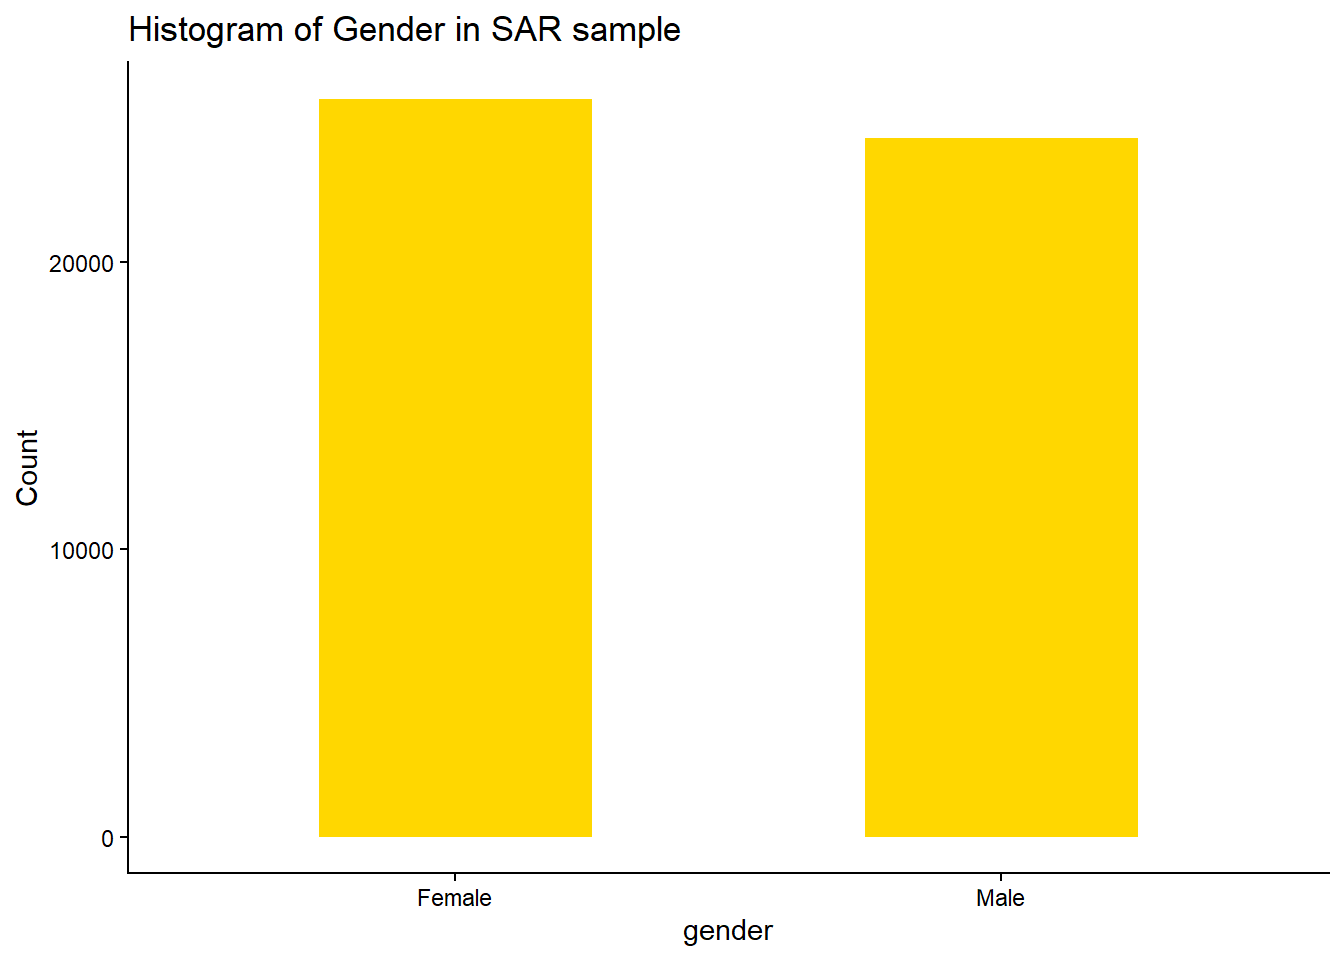
\includegraphics[keepaspectratio]{labs/04.LogisticRegression_files/figure-pdf/unnamed-chunk-26-1.pdf}}

\textbf{Answer for Q2}

Similarly, the descriptive analysis for the newly created variable
\texttt{New\_work\_distance}~in \texttt{sar\_df} should include:

\begin{Shaded}
\begin{Highlighting}[]
\FunctionTok{table}\NormalTok{(sar\_df}\SpecialCharTok{$}\NormalTok{New\_work\_distance)}
\end{Highlighting}
\end{Shaded}

\begin{verbatim}

    0     1 
29954  3072 
\end{verbatim}

Here we see the categories of \texttt{New\_work\_distance} are in
numeric type 0 or 1 (as we used code
\texttt{sar\_df\ \textless{}-\ sar\_df\ \%\textgreater{}\%\ mutate(\ New\_work\_distance\ =\ if\_else(work\_distance\ \textgreater{}6,\ 1,0))}
to do so), therefore in the histogram code, we use as.factor() to
convert it as factor type.

\begin{Shaded}
\begin{Highlighting}[]
\FunctionTok{ggplot}\NormalTok{(sar\_df, }\FunctionTok{aes}\NormalTok{(}\AttributeTok{x =} \FunctionTok{as.factor}\NormalTok{(New\_work\_distance))) }\SpecialCharTok{+}
  \FunctionTok{geom\_bar}\NormalTok{(}\AttributeTok{fill=}\StringTok{"forestgreen"}\NormalTok{,}\AttributeTok{width=}\FloatTok{0.5}\NormalTok{) }\SpecialCharTok{+}
  \FunctionTok{labs}\NormalTok{(}\AttributeTok{title =} \StringTok{"Histogram of New\_work\_distance in SAR sample"}\NormalTok{, }\AttributeTok{x =} \StringTok{"gender"}\NormalTok{, }\AttributeTok{y =} \StringTok{"Count"}\NormalTok{)}\SpecialCharTok{+}\CommentTok{\#set text info}
  \FunctionTok{theme\_classic}\NormalTok{()}\CommentTok{\#choose theme type, try theme\_bw(), theme\_minimal() see differences}
\end{Highlighting}
\end{Shaded}

\pandocbounded{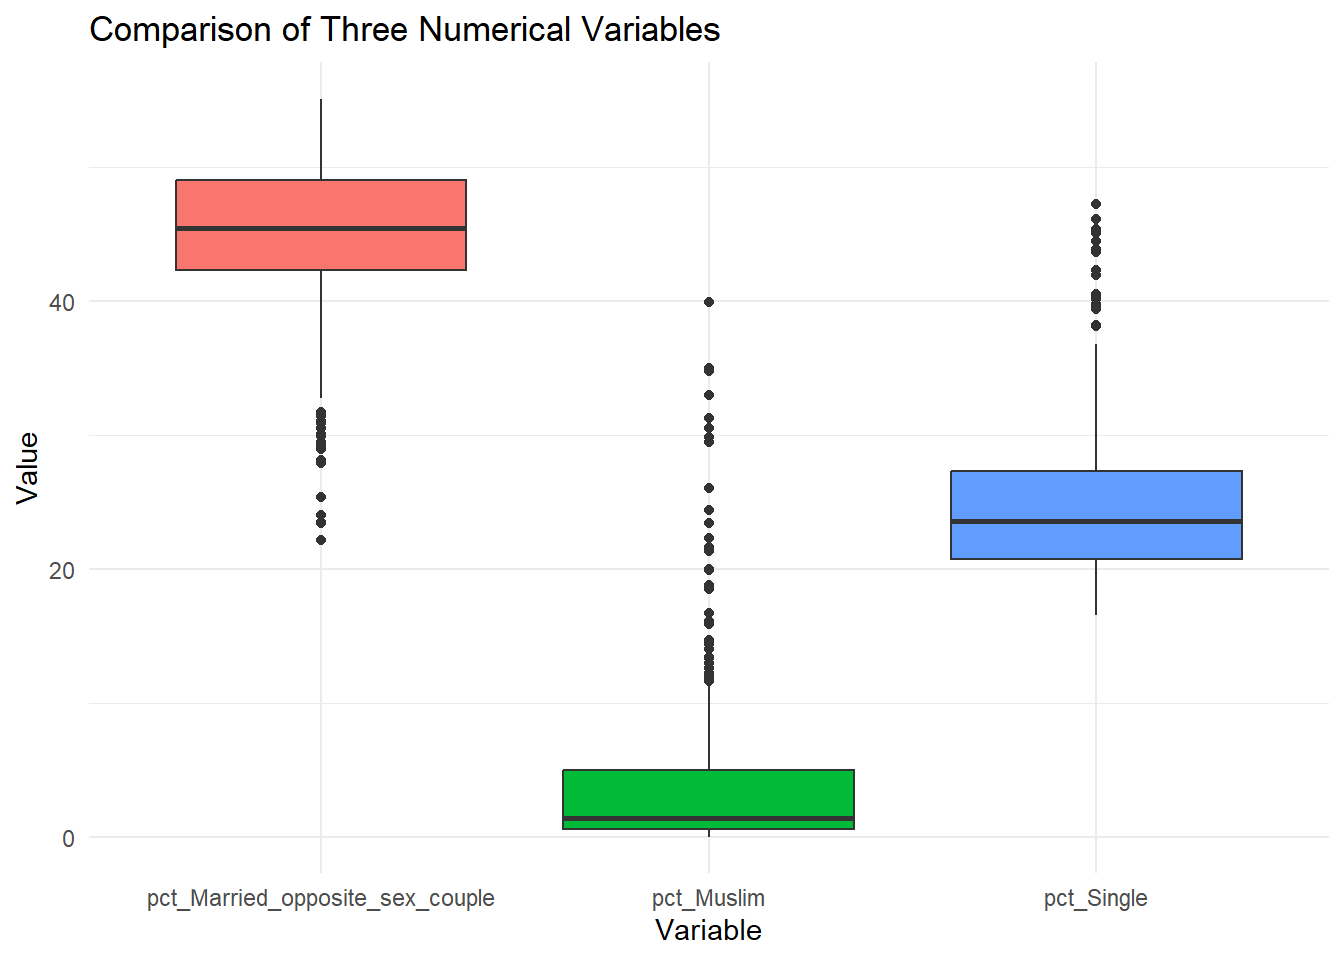
\includegraphics[keepaspectratio]{labs/04.LogisticRegression_files/figure-pdf/unnamed-chunk-28-1.pdf}}

Now we can use the frequency and the bar chart to report that according
to our definition of long-distance travelling to work (over 60 km),
there are 3072 individual are long-distance commuters in the SAR sample,
which makes up 6.14\% (3072/50000) of the sample.

\textbf{Answer for the model in Q4}

In Q4, we we want to explore whether people with occupation being
independent employers are associated with higher probability of
commuting over long distance when comparing to people in other
occupation. So we set the nssec= 5 (Small employers and own account
workers) as the baseline category.

\begin{Shaded}
\begin{Highlighting}[]
\FunctionTok{table}\NormalTok{(sar\_df}\SpecialCharTok{$}\NormalTok{New\_nssec)}
\end{Highlighting}
\end{Shaded}

\begin{verbatim}

    0     6     7     8 
20063  2790  5704  4469 
\end{verbatim}

Then we set the reference categories: \texttt{sex} as \texttt{1} (male)
and \texttt{New\_nssec} as 5, which is `Small employers and own account
workers':

\begin{Shaded}
\begin{Highlighting}[]
\NormalTok{sar\_df}\SpecialCharTok{$}\NormalTok{sex }\OtherTok{\textless{}{-}} \FunctionTok{relevel}\NormalTok{(}\FunctionTok{as.factor}\NormalTok{(sar\_df}\SpecialCharTok{$}\NormalTok{sex),}\AttributeTok{ref=}\StringTok{"1"}\NormalTok{)}
\NormalTok{sar\_df}\SpecialCharTok{$}\NormalTok{nssec }\OtherTok{\textless{}{-}} \FunctionTok{relevel}\NormalTok{(}\FunctionTok{as.factor}\NormalTok{(sar\_df}\SpecialCharTok{$}\NormalTok{nssec),}\AttributeTok{ref=}\StringTok{"5"}\NormalTok{)}
\end{Highlighting}
\end{Shaded}

Now, we build the logistic regression model and check out the outcomes:

\begin{Shaded}
\begin{Highlighting}[]
\NormalTok{model\_new }\OtherTok{=} \FunctionTok{glm}\NormalTok{(New\_work\_distance}\SpecialCharTok{\textasciitilde{}}\NormalTok{sex }\SpecialCharTok{+}\NormalTok{ nssec, }\AttributeTok{data =}\NormalTok{ sar\_df, }\AttributeTok{family=} \StringTok{"binomial"}\NormalTok{)}

\FunctionTok{summary}\NormalTok{(model\_new)}
\end{Highlighting}
\end{Shaded}

\begin{verbatim}

Call:
glm(formula = New_work_distance ~ sex + nssec, family = "binomial", 
    data = sar_df)

Coefficients:
            Estimate Std. Error z value Pr(>|z|)    
(Intercept) -0.44698    0.04138 -10.801   <2e-16 ***
sex2        -0.36678    0.04196  -8.742   <2e-16 ***
nssec2      -1.22639    0.06489 -18.898   <2e-16 ***
nssec1      -1.35519    0.10782 -12.569   <2e-16 ***
nssec3      -1.61400    0.05482 -29.442   <2e-16 ***
nssec4      -2.25717    0.07696 -29.329   <2e-16 ***
nssec6      -2.61631    0.10377 -25.212   <2e-16 ***
nssec7      -2.66548    0.08317 -32.047   <2e-16 ***
nssec8      -2.71172    0.09021 -30.059   <2e-16 ***
---
Signif. codes:  0 '***' 0.001 '**' 0.01 '*' 0.05 '.' 0.1 ' ' 1

(Dispersion parameter for binomial family taken to be 1)

    Null deviance: 20441  on 33025  degrees of freedom
Residual deviance: 17968  on 33017  degrees of freedom
AIC: 17986

Number of Fisher Scoring iterations: 6
\end{verbatim}

For the model interpretation, we need:

\begin{Shaded}
\begin{Highlighting}[]
\CommentTok{\# odds ratios}
\FunctionTok{exp}\NormalTok{(}\FunctionTok{coef}\NormalTok{(model\_new)) }
\end{Highlighting}
\end{Shaded}

\begin{verbatim}
(Intercept)        sex2      nssec2      nssec1      nssec3      nssec4 
 0.63955383  0.69296493  0.29335107  0.25789714  0.19909052  0.10464615 
     nssec6      nssec7      nssec8 
 0.07307217  0.06956621  0.06642224 
\end{verbatim}

\begin{Shaded}
\begin{Highlighting}[]
\CommentTok{\# confidence intervals}
\FunctionTok{exp}\NormalTok{(}\FunctionTok{confint}\NormalTok{(model\_new, }\AttributeTok{level =} \FloatTok{0.95}\NormalTok{)) }
\end{Highlighting}
\end{Shaded}

\begin{verbatim}
Waiting for profiling to be done...
\end{verbatim}

\begin{verbatim}
                 2.5 %     97.5 %
(Intercept) 0.58959085 0.69343772
sex2        0.63818099 0.75227729
nssec2      0.25813190 0.33291942
nssec1      0.20787318 0.31733101
nssec3      0.17876868 0.22162844
nssec4      0.08984430 0.12149367
nssec6      0.05933796 0.08915692
nssec7      0.05895858 0.08169756
nssec8      0.05547661 0.07902917
\end{verbatim}

And don't forget measure the model fit:

\begin{Shaded}
\begin{Highlighting}[]
\CommentTok{\# model fit}
\FunctionTok{pR2}\NormalTok{(model\_new) }\SpecialCharTok{\%\textgreater{}\%} \FunctionTok{round}\NormalTok{(}\DecValTok{4}\NormalTok{) }\SpecialCharTok{\%\textgreater{}\%} \FunctionTok{tidy}\NormalTok{()}
\end{Highlighting}
\end{Shaded}

\begin{verbatim}
fitting null model for pseudo-r2
\end{verbatim}

\begin{verbatim}
Warning in tidy.numeric(.): 'tidy.numeric' is deprecated.
See help("Deprecated")
\end{verbatim}

\begin{verbatim}
# A tibble: 6 x 2
  names              x
  <chr>          <dbl>
1 llh       -8984.    
2 llhNull  -10220.    
3 G2         2473.    
4 McFadden      0.121 
5 r2ML          0.0721
6 r2CU          0.156 
\end{verbatim}

\textbf{Q5.} \textbf{Now what conclusion you can draw when comparing the
median NSSEC groups to the higher groups?}




\end{document}
